\documentclass[instructions]{uqthesis}	%Use this option to include template instructions in the output.
%\documentclass[final]{uqthesis}				%Use this option to suppress the template instructions in the output.
%This is the UQ thesis template.
%See README for version.
\usepackage{textcomp}
\usepackage[utf8]{inputenc}
\usepackage{gensymb}
\usepackage{graphicx}
\usepackage{amssymb}
\usepackage{amsmath}
\usepackage{bm}
\usepackage{float}
\usepackage[scientific-notation=true]{siunitx}
\usepackage{caption}
\captionsetup{justification=raggedright,singlelinecheck=false}
\usepackage{booktabs}
\renewcommand{\arraystretch}{1.25}


%You must have the memoir class installed.
%
%Be sure to observe the content of comments within the source code.
%Most important instructions have been CAPITALISED.
%
%Please see the README for more information!

%This file loads the necessary packages, sets the page styles, and defines a bunch of macros.
%Edit this if you are comfortable with LaTeX.
%Other tweaks can be made in uqthesis.cls, but monkey with these at your own risk!
\input{style.tex}

% ***************************************************
% You should specify the contents of title page here
% ***************************************************
%Add your thesis title here. USE SENTENCE CASE (capitalise only the first word and proper nouns).
\title{Distributed parameter modelling of phototrophic systems}

%YOUR NAME.
%Do not include initials or middle names. Do not include your supervisor(s)' name(s).
\author{Edward Barry}
%YOUR CURRENT DEGREES.
%Use abbreviations. Do not include the date or location of your degree. Do not include the degree for which this thesis is being submitted.
\currentdegrees{B.Eng. (Hons)}

%YEAR OF SUBMISSION.
\date{2018}
%TYPE OF DEGREE you are submitting for.
\submittedfor{Doctor}

%ADD YOUR SCHOOL.
%Use title case (capitalise every word which is not a conjunction or preposition).
%See http://blog.apastyle.org/apastyle/2012/03/title-case-and-sentence-case-capitalization-in-apa-style.html for help.
\school{School of Chemical Engineering}

\begin{document}

\frontmatter
% *************** Assemble title page ***************
\maketitle
\clearpage

% ***************************************************
\section{Abstract}
\normalfont
%OPEN ABSTRACT.TEX TO EDIT.
% %TO PRODUCE A STAND-ALONE PDF OF YOUR ABSTRACT, un-comment this header and the \end{document} at the end of the file.
% %
%\documentclass[12pt, a4paper]{memoir}
%
%\usepackage{mathptmx}
%\input{../style.tex}
%
%\begin{document}
%
%\begin{center}
	%\textbf{\large Your title goes here}
	%
	%\textbf{Abstract}
	%
	%Your Name, The University of Queensland, 20??
%\end{center}

%WRITE YOUR ABSTRACT HERE.
Purple phototrophic bacteria (PPB) use infrared light to generate microbial energy, with electron, carbon, and nitrogen supplied chemically. They have broad applicability for resource recovery from wastes and wastewater, as they have potential value as microbial product, and very high growth yields on substrate. Although PPB processes are gaining relevance in the aforementioned industries, reactor design, particularly effective consideration of light in chemical kinetics and hydraulics is a critical issue. This thesis aims to assess key limitations and define their physical behaviour mathematically. The first limitation was that there was no mixed culture PPB process model describing the behaviour of PPB in the presence of ammonia, organic matter, and other nutrients. The mixed population models of the International Water Association (IWA) provide a good framework for process modelling and control. As such, a process model for a mixed-culture PPB system was developed based on five key processes: photoheterotrophic growth, photoautotrophic growth, chemoheterotrophic growth, hydrolysis/fermentation, and decay. This model was developed as a set of ordinary differential equations varying in time, and lumped in space (as for the IWA models). The second limitation is that the radiative field has not been considered. This can vary spatially and temporally. The radiative field in a PPB system attenuates sharply, which influences the growth domains. A CFD modelling framework was therefore developed in OpenFOAM to describe the spatial variations and interactions between biomass growth, the flow field, and the radiative field. It was found that lumped modelling approaches and distributed parameter approaches differed in results based on different reactor domains and behaviours. The deviation from lumped parameter behaviour was greater for a cylindrical stirred reactor than for a flat plate reactor. Therefore, spatial considerations are necessary in the design phase of a photobioreactor. Finally, biofilms are a critical aspect in PPB growth, and a coupled biofilm-radiative model has not been previously considered. The model was thus extended to include biofilm formation of a mixed PPB system in the presence of a spatially varying radiative field. A volume-of-fluid approach was used as a basis for this model, considering three particulate species (phototrophic bacteria, biodegradable particulate matter, and inert particulates \textbf{Throw in results section from final chapter here}). The radiative-solid-liquid coupling overall was found to be critical in operation, with traditional lumped parameter approaches to design and analysis not well suited to the emerging challenges of mixed culture photo-bio systems. These aspects should be further considered through model based analysis and experimental validation for future system design.

%\end{document}

\clearpage
% ***************************************************
\section*{Declaration by author}
%DO NOT EDIT.
\input{copyrightstatement.tex}

\clearpage
%YOU MUST EDIT THIS DOCUMENT.
% ***************************************************
\section*{Publications included in this thesis}

%\begin{instructional}

%	Start this section on a new page [this template will automatically handle this].
	
%	If you choose to include publications as part of your thesis as described in UQ policy (\href{http://ppl.app.uq.edu.au/content/4.60.07-alternate-thesis-format-options}{PPL 4.60.07 Alternative Thesis Format Options}) use this section to detail accepted or in press publication/s using the standard citation format for your discipline. 

%	Papers submitted for publication and awaiting review should appear in the next section, \textbf{Submitted manuscripts included in this thesis}.

%	On the page immediately preceding the chapter that includes your publication, in no more than one (1) page, describe your contribution to the authorship if you are not a sole author. In describing your contribution, you must satisfy the University's authorship policy (\href{http://ppl.app.uq.edu.au/content/4.20.04-authorship}{PPL 4.20.04 Authorship}). Authorship is based on having made a substantive contribution to at least one, and usually more than one, of the following activities:
	%
%	\begin{itemize*}
%		\item	conception and design of the project;
%		\item	analysis and interpretation of the research data on which the publication is based;
%		\item	drafting significant parts of the publication or critically reviewing it so as to contribute to the interpretation.
%	\end{itemize*}
	
%	As an author, you must have participated sufficiently in the publication to take public responsibility for at least that part of the work that you contributed.

%	It may be useful to refer to specific parts of the methods, analyses, results, or discussion to illustrate your contribution to the paper.

%	If you have not included any of your publications in the thesis then state ``No publications included''.
	
%	\eg{} could set out like so:
%\end{instructional}

%\begin{enumerate}

%\item \cite{citationkey} \textbf{Your Name}, Co-author 1, and Final Author, \href{linktoyourpaper}{Title of your paper}, \textit{Journal}, Issue, Number, Year

%\item \cite{citationkey} \textbf{Your Name}, Co-author 1, and Final Author, \href{linktoyourpaper}{Title of your paper}, \textit{Journal}, Issue, Number, Year

%\end{enumerate}

% ***************************************************
\section*{Submitted manuscripts included in this thesis}

%\begin{instructional}
%	List manuscript/s submitted for publication here. As described above for \textbf{Publications included in the thesis}, on the page immediately preceding the chapter that includes the submitted manuscript, in no more than one (1) page, detail your contribution to the authorship if you are not the sole author.

%If you have no submitted manuscripts from your candidature then state ``No manuscripts submitted for publication''.

%\eg{} you could set out like so:
%\end{instructional}

%\begin{enumerate}

%\item \cite{citationkey} \textbf{Your Name}, Co-author 1, and Final Author, Title of your paper, submitted to \textit{Journal} on 4th June 2018.

%\end{enumerate}

% ***************************************************
\section*{Other publications during candidature}

%\begin{instructional}
%List other publications arising during your candidature using the standard citation format for your discipline. Divide your %publications into sub-sections as appropriate in your discipline \eg{} peer-reviewed papers, book chapters, conference %abstracts. Papers submitted for publication and awaiting review are not considered publications and cannot be included in this %section.

%If you have no publications from your candidature then state ``No other publications''.

%\eg{} you could set out like so:
%\end{instructional}

% ***************************************************
\subsection*{Conference abstracts}

%\begin{enumerate}

%\item \cite{citationkey} \textbf{Your Name}, Co-author 1, and Final Author, Title of your conference paper, \textit{Proceedings of Conference}, other details.

%\end{enumerate}

% ***************************************************
\subsection*{Book chapters}

%\begin{enumerate}

%\item \cite{citationkey} \textbf{Your Name}, Co-author 1, and Final Author, Title of your chapter, Book, editor, \etc{}.

%\end{enumerate}

% ***************************************************
\section*{Contributions by others to the thesis}

My advisory team of Prof. Damien Batstone, A/Prof. Christopher DeGroot, and Dr. Tim H\"{u}lsen provided feedback on the wrok presented. A/Prof. Christopher DeGroot contributed to some development at the early stages of the research project, and was instrumental in help with debugging as a set of fresh eyes towards the end of the research project.

% ***************************************************
\section*{Statement of parts of the thesis submitted to qualify for the award of another degree}

No works submitted towards another degree have been included in this thesis.

% ***************************************************
\section*{Research involving human or animal subjects}

No animal or human subjects were involved in this research.

\clearpage

% ***************************************************
\section*{Acknowledgments}

%\begin{instructional}
%Start this section on a new page [the template will handle this for you].

%Acknowledgements recognise those who have been instrumental in the completion of the project.  Acknowledgements should include any professional editorial advice received including the name of the editor and a brief description of the service rendered.
%\end{instructional}

\clearpage

% ***************************************************
\section*{Financial support}

%\begin{instructional}
%Start this section on a new page [the template will handle this for you].

%If you are the recipient of an Australian Government Research Training Program (RTP) scholarship, you are required to acknowledge this contribution.  Please include the text below:

%``This research was supported by an Australian Government Research Training Program Scholarship''

%If you received any other financial support for your project, you are also required to acknowledge the funding body/bodies in this section.

%If no financial provided then state ``No financial support was provided to fund this research''.
%\end{instructional}

%No financial support was provided to fund this research.

% ***************************************************
\section*{Keywords}

%\begin{instructional}
%	Maximum 10 words; use lower case throughout, separating words/phrases with commas. For example:
%\end{instructional}

Computational fluid dynamics, purple phototrophic bacteria, process modelling, mechanistic modelling, biofilms, 

\section*{Australian and New Zealand Standard Research Classifications (ANZSRC)}

%\begin{instructional}
%Provide data that links your thesis to the disciplines and discipline clusters in the Federal Government’s Excellence in %Research for Australia (ERA) initiative.

%Please allocate the thesis a \textbf{maximum of 3} %\href{http://www.abs.gov.au/Ausstats/abs@.nsf/Latestproducts/6BB427AB9696C225CA2574180004463E?opendocument}{Australian and New %Zealand Standard Research Classifications (ANZSRC) codes} at the \textbf{6 digit level} and include the descriptor and a %percent weighting for each code. Total percent must add to 100.

%Example:
%\end{instructional}

\noindent
ANZSRC code: 091501, Computational Fluid Dynamics, 50\% \\
ANZSRC code: 090702, Environmental Engineering Modelling, 40\% \\
ANZSRC code: 090409, Wastewater Treatment Processes, 10\%


% ***************************************************
\section*{Fields of Research (FoR) Classification}
%
%\begin{instructional}
%Allows for categorisation of the thesis according to the field of research. 
%
%Please allocate the thesis a \textbf{maximum of 3} %\href{http://www.abs.gov.au/Ausstats/abs@.nsf/Latestproducts/6BB427AB9696C225CA2574180004463E?opendocument}{Fields of Research %(FoR) Codes} at the \textbf{4 digit level} and include the descriptor and a percent weighting for each code. Total percent must %add to 100. 
%
%Example:
%\end{instructional}

FoR code: 0915, Interdisciplinary Engineering, 50\% \\
FoR code: 0907, Environmental Engineering, 40\% \\
FoR code: 0904, Chemical Engineering, 10\%
\clearpage

%If you wish to add a dedication (if appropriate), do so here.
%If not, comment out from here...
%	\rmfamily
%	\normalfont

%	\begin{vplace}[1]
%		\begin{center}
%			This template is dedicated to nerds everywhere.
%		\end{center}
%	\end{vplace}

%... to here.

%\clearpage
\pagestyle{headings}

%These generate the table of contents, list of figures, and list of tables from items tagged with a \label{} command.
\tableofcontents
	\clearpage
\listoffigures
	\clearpage
\listoftables

% *************** List of abbreviations ***************

% ******************************************************************************
% You can make a list of abbreviations here.
%
% You only need to make a label when a symbol is introduced in the document and
% here you can reference this label to obtain page number.
%
% There are LaTeX packages available to take care of these things, but you will
% need to manually add these to the template at this stage (support may be added
% in future releases).
% ******************************************************************************

%CHOOSE THE APPROPRIATE TITLE.
%\chapter[List of abbreviations]{List of abbreviations}
\chapter[List of abbreviations and symbols]{List of abbreviations and symbols}

%If the auto-sizing of the tables annoys you, consider the tabularx package.

%List of abbreviations.
\begin{center}
	\small
	\begin{longtable}{ll}
	\toprule
	Abbreviations & {} \\
	\bottomrule
ADMn &	Anaerobic digestion model (nth release) \\
ASMn &	Activated sludge model (nth release) \\
CFD &	Computational fluid dynamics \\
COD &	Chemical oxygen demand \\
CR &	Cylindrical reactor \\
DOM &	Discrete ordinates method \\
FPR &	Flat plate reactor \\
FvDOM &	Finite volume discrete ordinates method \\
FVM &	Finite volume method \\
HG &	Henyey-Greenstein phase function \\
HPC &	High performance computing \\
IWA &	International Water Association \\
LH$n$ &   Light harvesting apparatus $n$; $n \in \{1, 2\}$ \\
MC &	Monte Carlo \\
NIR &   Near-infrared radiation \\
ODE &	Ordinary differential equation \\
PAR &	Photosynthetically active radiation \\
PBR &	Photobioreactor \\
PDE &	Partial differential equation \\
PPB &	Purple phototrophic bacteria \\
PSU &	Photosynthetic unit \\
RANS &	Reynolds-averaged Navier-Stokes \\
RC  &  Reaction centre \\
RPM &	Revolutions per minute \\
RTE &	Radiative transfer equation \\
SM  &	Schlick model \\
SST &	Shear stress transport \\
TPF &	Truncated phase function \\
	\hline
	\end{longtable}
\end{center}

%List of symbols. REMOVE IF NOT NEEDED.
\begin{center}
	\small
	\begin{longtable}{ll}
	\toprule
	Symbols & {} \\
	\bottomrule
	$\hat{\rho}$		& Density operator \\
	\etc{}					& \etc{} \\
	\hline
	\end{longtable}
\end{center}

% *************** End of list of symbols and abbreviations ***************

% *************** End of front matter ***************

% ********* Main matter begins ***************
\mainmatter

%Each chapter is a separate .tex file. Use \input to load them here.
%I recommend keeping each in a separate subfolder, along with its accompanying figures, etc. This is how the file is currently structured.
%
%If you wish to divide your thesis into parts (each containing multiple chapters), us the \part{} command.



% *************** CHAPTER 1 ***************
\chapter[Introduction]{Introduction}
\label{chap:chap1}
\section{Motivation}
\label{sec:chap1-motivation}
Purple phototrophic bacteria (PPB) have recently been proposed as an effective biotechnology for engineered applications including the treatment of domestic \cite{Hulsen2016} and industrial wastewaters \cite{Hulsen2018}. Phototrophic bacteria, along with their chromaphores, have also shown promise in a range of highly valued end products such as animal feeds \cite{Sun2016}, biofuels \cite{Adessi2014}, and even cosmetic and pharmaceutical products\cite{Liu2013, Wang2018}. Despite the increasing interest in these applications, they have not achieved widespread implementation largely due to the gaps in collective knowledge at the process level. In particular, the description and quantification of the interactions between biochemical behaviour, irradiation, and fluid hydrodynamics have proven to be significant design bottlenecks when scaling up photobioreactors. 
\skippingparagraph
\noindent By approaching the problem with a semi-mechanistic modelling approach, one can better understand these interactions and how their behaviour can influence the design and optimisation decisions at scale up. As such, this thesis aims to explore the current state of process modelling, computational fluid dynamics, and radiative transfer modelling and combine these concepts into a unified distributed parameter modelling framework for phototrophic systems and photobioreactors.  Additionally, a deterministic, semi-mechanistic biofilm model is developed which draws upon the physical phenomena identified is also developed in response to the need to find a solution to engineering challenges associated with biomass harvesting. 


%------------------------------------------------------------------------------%
%------------------------------------------------------------------------------%
%------------------------------------------------------------------------------%



%------------------------------------------------------------------------------%
%------------------------------------------------------------------------------%
\newpage
\section{Background}
\label{sec:chap1-background}
\subsection{Time varying wastewater treatment models}
\label{ssec:chap1-wwtmod}
Models use mathematical expressions to explain the underlying processes or inputs of outputs of a system \cite{Hangos2001}. They can be classed according to the method of their development. When developing process models, a number of decisions can be made depending on the nature of the model and the information required for understanding.
\begin{itemize}
    \item Mechanistic or empirical models
    \item Continuous or discrete models
    \item Lumped parameter (well-mixed) or distributed parameter models
    \item Stochastic or deterministic models
\end{itemize}

In reality, a model can be made using a combination of these different categories, depending on the target use of the model. Most of the available literature for wastewater treatment models is concerned with semi-mechanistic, continuous, lumped parameter and deterministic approaches to modelling. The major generic models in the domain of wastewater treatment, from which this thesis branches, are the International Water Association (IWA) family of models. These include the activated sludge model family, and the anaerobic digestion model (ADM) \cite{Batstone2006} family. These have been combined together with appropriate unit process models such as clarifier models \cite{Takacs1991} into standardised plant-wide models \textbf{BSM}. Modelling of wastewater treatment processes can lead to a greater understanding of the underlying physics and biochemistry \cite{Szilvester2010}. All IWA models are semi-mechanistic, which means that the model equations are based on known mechanistic phenomena, such as the presence of known biological clades, but the kinetic relationships are generally empirical.
\skippingparagraph
These models are useful in understanding the underlying biochemical processes occurring on wastewater treatment systems. They also serve as good tools for process unit design in wastewater treatment plants. The benefits of these models are that they are readily extensible, and allow themselves to be used in distributed parameter models \cite{Batstone2006a}. This also means that the IWA models can be applied for PPB time-series and distributed parameter models in contexts broader than just wastewater treatment. 
\subsubsection{Purple phototrophic bacteria growth models}
Purple phototrophic bacteria are some of the most metabolically versatile organisms on earth \cite{Hunter2008}. They have been shown to grow well as photoheterotrophs under anaerobic conditions \cite{Hulsen2014}. They also grow chemoheterotrophically in the absence of irradiation, and they grow photoautotrophically using irradiance to drive $\mathrm{CO_2}$ fixation \cite{Gordon2014}. With respect to the modelling of phototrophic bacteria, there currently exist no models in the context of wastewater treatment and industrial growth in mixed systems on nutrients and organics, however the suite of metabolic modelling of PPB is rich but not readily applicable for a process engineering perspective \cite{Klamt2002}.
\subsubsection{Purple phototrophic bacteria and radiation modelling}
PPB have evolved to efficiently harvest available solar radiation in aquatic environments \cite{Cogdell2006a}. Due to oxygenic photosynthetic organisms filtering radiation in the visible band in the upper aerobic zones of these aquatic systems, PPB have adapted to make use of remaining solar energy, which include green and near infra-red (NIR) radiation \cite{Cogdell2006a}. The light harvesting apparatus in \textit{Rhodobacterales} consists of two light harvesting complexes (LH2 and LH1), and a reaction centre (RC) \cite{Hellingwerf1994}. A useful abstraction of the light harvesting complex is two distinct zones (LH2 and an LH2-RC complex) with absorbance spectra at 800-850 \si{nm} and 880 \si{nm} respectively. Figure \textbf{cite: figure} demonstrates how these light harvesting centres are arranged and how they participate in providing energy to the electron transport chain to ultimately generate ATP for growth and other cell processes. \textbf{DRAW A LHC SCHEMA IN LODRAW}.
\skippingparagraph
In terms of modelling PPB and their interactions with photons for industrial applications, very little has been done. Most studies focusing on photobioreactor design have been for hydrogen production applications \cite{Adessi2014, Krujatz2015}. Further limitations to these works were that particular wavelengths were not selected, with most opting for direct sunlight or white tungsten or halogen lamps as light sources. These approaches are problematic for a wastewater treatment application, as the use of broad spectrum light will leads to competition by other heterotrophic bacteria, and other phototrophic and photosynthetic organisms found in domestic wastewater such as algae and cyanobacteria.
\skippingparagraph

Efforts were made to combine a mass balance approach to the photoheterotrophic efficiency of PPB \cite{Minkevich2004}. In this work, theoretical and experimental yields of purple phototrophic bacteria were calculated based on different electron donors and light sources. The maximum theoretical yields based on acetate as an electron donor are summarised in Table~\ref{tab:theoreticalQuantum}, where $Y^m_{X/LE}$ is the maximum biomass growth per light energy dose;

\begin{table}[H]
  \begin{center}
    \caption{Maximum theoretical \textit{Rb. capsulatus} yield with
      acetate as electron donor for different wavelengths
      \cite{Minkevich2004}}
    \label{tab:theoreticalQuantum}
    \begin{tabular}{ | l | l |}
      \hline
      Wavelength& $Y^m_{X/LE}$ ($gVSS\cdot kJ^{-1}$)\\ \hline \hline
      860 nm & 0.020 \\ \hline
      744 nm & 0.017  \\ \hline
      522 nm & 0.012  \\ \hline
    \end{tabular}
  \end{center}
\end{table}

The theoretical model was then compared to experimental data, with the
following values obtained through experiment. This information is
presented in Table~\ref{tab:expQuantum}.

\begin{table}[H]
  \begin{center}
    \caption{PPB experimental yield for different wavelengths and
      lactate and acetate as electron donors\cite{Minkevich2004}}
    \label{tab:expQuantum}
    \begin{tabular}{ | l | l | l | l |}
      \hline
      \textbf{Species} & \textbf{Wavelength} & \textbf{Electron donor} & $Y_{X/LE}$ ($gVSS\cdot kJ^{-1}$)\\ \hline \hline
      \textit{Rb. capsulatus} & 860 nm & lactate & 0.018 - 0.031 \\ \hline
      \textit{Rb. sphaeroides} & White ($\bar{\lambda}$ = 744 nm) & acetate & 0.009 - 0.016 \\ \hline
      \textit{Rb. capsulatus} & 522 nm & lactate & 0.006 - 0.013 \\ \hline

    \end{tabular}
  \end{center}
\end{table}
	
The data of \cite{Minkevich2004} serves as an effective basis for quantifying and understanding the interactions between biomass growth, maintenance and decay, and the irradiance required for optimal reactor performance.

\textbf{Operating parameters from Berberoglu and Pilon, and Murphy and Berberoglu and Hale and Querrey}.


\subsection{Computational fluid dynamics for wastewater treatment and photobioreactors}
Traditional design methods of wastewater treatment process units consist of load and mass based static analysis, and testing of dynamic behaviour based on key operating state variables \cite{Gaden2013}. Computational fluid dynamics (CFD) is a cost-effective method for scaling up process units and testing variations in operating parameters. This allows the design of equipment without needing physical prototypes \cite{Wood1995}. CFD involves the spatiotemporal numerical analysis of transport equations and chemical reactions \cite{versteeg2007}. There have been many applications for CFD, including aerodynamic studies of aircraft, turbine analysis in power plants, environmental modelling of pollutants, and biomedical analysis of blood flows \cite{Versteeg1995}. The major CFD studies in water treatment modelling have been conducted in the fields of algae growth, the inactivation of pathogens by ultraviolet radiation, and geometry and flow optimisation of conventional treatment plant units such as clarifiers, ponds and digesters. These areas of application have been chosen as a basis for literature review, due to photobioreactors operating with similar physical phenomena such as radiation delivery, multiphase fluid flows, and biochemical reactions \cite{Bitog2011}. 


\subsubsection{Bubble Column Models}
There are numerous studies looking at modelling bubble columns in a spatio-temporal manner. One of the early works in this field identified a need to consider a modelling technique incorporating spatio-temporal variations in order to minimise capital and operating costs during scale-up of general bubble column reactors \cite{Lapin1994}. In this study, the Navier-Stokes system of equations modelled the continuous fluid phase, and the dispersed gas bubbles were modelled as discrete tracked particles, with their position being solved over time. As this was a 1994 study, the computing power limited the model development to a two dimensional 60 x 200 grid of a $0.75 m^{2}$ reactor face. Numerical diffusion arose when both the liquid and gas were considered as continuous phases. With the improvement in desktop computing capacity, CFD has been used extensively for bubble column and airlift reactor validation using both approaches \cite{Bitog2011}. Other studies have looked at describing bubble flow within different reactor geometries with Eulerian-Eulerian (both phases considered continuous) methods \cite{Lehr2002, Pfleger2001, Buwa2002, Pareek2003, Ekambara2005, Sokolichin1999}. Gas-liquid flow in bubble columns has also been investigated with Eulerian-Lagrangian (continuous liquid phase and discrete gas phase) models \cite{Zhang2013a}. The major works in this field have looked at different geometry bubble columns with drag force, virtual mass force, lift force primarily with two dimensional geometries \cite{Buwa2006, Goz2004a, Luo2011, Ekambara2005, Lan2002, Mouza2004}. These studies looked at the sensitivity of the columns to such parameters and conditions as turbulence model, sparger location, superficial gas velocity, reactor aspect ratio and virtual mass.
\skippingparagraph

\textbf{\textit{Limitations of Bubble Column Studies}} \\
The main strength of these bubble column CFD models is that they are applied to general simple geometries, as the main focus was to isolate the bubble flows to explain the effects of the principal hydrodynamic operating conditions and parameters. These general approaches to CFD modelling of bubble columns present a strong platform from which to commence photobioreactor simulations, but they also lead to limitations in the context of purple phototrophic bacteria for wastewater treatment. Even if solids are present in the system being modelled, phases are modelled as liquid and gas. Modelling approaches for solid phases require refinement, in which the solids are modelled as discrete particles, and the liquid and gas phases are modelled as continuous phases. In addition, these cases used simple geometries, which will probably not be appropriate for photobioreactor modelling and design, as the irradiated surface to volume ratio plays an important role in reactor performance \cite{Soman2015}. Another note is that the generality of these cases means that biochemical reactions and photon-biomass interactions were not included in the studies. 
\skippingparagraph

Phototrophic microorganisms pose promising solutions to current important technological challenges: the management of wastes such as atmospheric pollutants and wastewater, production of high value products from waste streams, such as biofuels and bio-plastics \cite{Hulsen2016}. They are resilient under favourable radiative conditions, quickly out-competing other non photosynthetic organisms \cite{Posten2009}. Photosynthetic and phototrophic microorganisms can be used in photobioreactors (PBR), which can be categorised based on whether the reactor is situated indoors or outdoors, its geometry (tubular, flat plate, raceway), whether it is anaerobic or aerobic, and the method of mixing (sparged, paddle wheel). The technology for these various applications has however not been widely adopted, partly due to gaps in understanding of good PBR design, and partly due to energy and utilities markets not being favourable to large scale implementations. A method to address the former is to undertake virtual prototyping using computational fluid dynamics CFD \cite{Bitog2011}. This allows rapid development and experimentation, without the traditional expenses incurred in the scale up process \cite{Bridgeman2012}.
\skippingparagraph

The use of CFD for PBR analysis has increased since the first few studies in the early 1980s \cite{Patankar1980}. Wider access to commercial CFD software packages and suitable computational resources are likely factors in this uptake. Commercial packages allow the user to streamline the work flow from geometry design, to meshing, to case set up, to data analysis and visualisation. One must however be prudent when carrying out CFD studies of PBRs, because the automation and ease in setting up cases with commercial packages could lead to undesirable or even non-validated and inaccurate solutions. Such issues of good CFD modelling practice and uncertainty quantification have been well documented in industries with a longer history of CFD usage \cite{Roache2002,Oberkampf2002,Celik2008,Pelletier2010}.  More recently, efforts have been made to outline good CFD modelling practices in the context of wastewater treatment plants \cite{Wicklein2016}.
\skippingparagraph

CFD modelling has aided in the understanding of hydrodynamic processes, and a comprehensive review was carried out in 2011 reflecting the status of CFD modelling of PBRs \cite{Bitog2011}. Most papers reviewed focused on the implications of certain geometry designs on flow characteristics. The papers were sampled to find a consensus on the use of a turbulence model. It was found that all studies reported used Reynolds-average Navier-Stokes (RANS) models, with the most popular being the standard $k-\epsilon$ model. The popularity of RANS models is not surprising, owing to their efficiency compared to more complex turbulence models.  The ubiquitous use of the standard $k-\epsilon$ model is somewhat surprising, given the evidence which shows this model is quite poor in predicting separated flows \cite{Menter2003}. Further, it is clear that improved $k-\epsilon$ models, such as the realizable $k-\epsilon$ model \cite{Shih1995}, as well as other improved RANS models, such as the $k-\omega$  SST model \cite{Menter1994,Menter2003} have been developed to address such deficiencies.
\skippingparagraph

The goal of this review is to not only provide an update in the state of the art CFD modelling practices, but to focus on the coupling and interactions between pertinent physical phenomena in PBR systems. Categories have been organised based on these physical processes, including hydrodynamics, radiation, biokinetics, porous media modelling for membrane and biofilm systems, and attempts to couple these processes. In addition, attention must be paid to analytical approaches including discretisation error evaluation. Guidelines from the Journal of Fluids Engineering can be adapted to this review \cite{Celik2008}.
\skippingparagraph

This work is based the recommendations presented by \cite{Posten2009}, and will assess CFD for PBR based on the following performance indicators that were highlighted: mixing, ``light'' delivery, mass transfer (including $CO_2$ delivery and $O_2$ purging in the case of micro-algae), and total energy demand. The study also alluded to the necessity in understanding and using the interactions between mass and radiative transfer, physiology of the microorganism in question, and their radiation and substrate kinetics and dynamics. In addition to these components, we have also identified that biofilm formation is important, whether one wants to avoid it, or use it as a design feature \cite{Castro2017}.

\begin{itemize}
\item hydrodynamics, including mixing and mass transfer
\item radiative transfer
\item phyisiology and biokinetics
\item biofilms
\item methods for coupling all physical phenomena
\item analysis of error and grid convergence
\end{itemize}

The solution for the flow of a fluid is obtained by numerical solution of the Navier-Stokes equations, along with addition models, as required, to account for multiple phases, turbulence, etc. Most often, the equations are discretised using a finite volume method (FVM), but can also be discretised using other methods such as the finite element, finite difference, or spectral methods.  The most common CFD packages for PBR studies are ANSYS Fluent and ANSYS CFX, both of which are based on FVM.  Although it has not been used extensively for CFD analysis of PBRs, OpenFOAM is another FVM-based CFD code which is open source.

\subsubsection{Turbulence Modelling}

\begin{itemize}
\item RANS modelling
\item Wall functions
\end{itemize}


\subsubsection{Modelling of gas phases}
\begin{itemize}
\item DNS
\item Eulerian
\item VOF
\end{itemize}

\subsubsection{Modelling of dispersed biosolid phases}
\label{S:21}

In general, there are two methodologies, Eulerian and Lagrangian, that can be implemented to solve the transport of a dispersed solid phase within continuous fluid phase(s) in a CFD simulation. The Eulerian approach treats the solid phase as a continuum and computes the concentration distribution based on the solution of a PDE that generally includes convective and diffusive terms, and may include various source and sink terms as required.  The Lagrangian approach, on the other hand, involves the calculation of a large number of particle trajectories, based on Newton's second law, and models of all forces acting on the particles, such as drag, lift, and gravity. Each method has its own advantages and disadvantages, and, depending on the specific objectives of the study, one method may be more appropriate or efficient than the other.  After outlining the details of each, recommendations will be made regarding the suitability of each for modelling PBR systems.
\skippingparagraph
In the Eulerian modelling approach, the flow field and concentration distribution of the particulate phase are calculated in sequence.  The PDE governing the particle phase concentration is \cite{Zhang2007} (add more references)

%%%%%%%%%%%%%%%%%%%%%%%%%%%%%%%%%%%%%%%%%%%%%%%%%%%%%%%%%%%%%%%%%%%%%%%%%%%%
%      INSERT THE EULERIAN PDE FOR PARTICLE PHASE CONCENTRATION 
%%%%%%%%%%%%%%%%%%%%%%%%%%%%%%%%%%%%%%%%%%%%%%%%%%%%%%%%%%%%%%%%%%%%%%%%%%%%
\begin{equation}
\frac{\partial C}{\partial t}
+ \nabla\cdot\left(\mathbf{u} C\right)
= \Gamma\nabla^2 C
+ S_c
\label{eq:eulerian_pde}
\end{equation}


The second term on the left side of Eq.\ \ref{eq:eulerian_pde} represents convection of the particles with the velocity of the fluid phase(s), coupling the flow and concentration fields.  This coupling is one-way since the solids concentration does not influence the flow field.  The first term on the right side of Eq.\ \ref{eq:eulerian_pde} represents diffusion, while the second term represents all sources and sinks.

Discuss diffusion coefficient

Discuss relative motion of solid wrt fluid and drift flux

Equation based on \cite{Zhang2007}; check other sources to ensure it's general.
%
\begin{equation}
	\frac{d\mathbf{u}_p}{dt}
    = F_D\left(\mathbf{u}-\mathbf{u}_P\right)
    + g\frac{\rho_p-\rho}{\rho_p}
    + \mathbf{F}_a
	\label{eq:lagrangian_ode}
\end{equation}

\subsubsection{Comparison of Eulerian and Lagrangian Methodologies}

The Eulerian and Lagrangian approaches have been compared previously for particle transport in enclosed air spaces \cite{Zhang2007} (others?). Here the comparison is considered specifically in the context of PBR systems.


%---------------------------------------------------------------------------------------------------
%%%%%%%%%% RADIATION MODELLING
%---------------------------------------------------------------------------------------------------
\subsection{Radiation Modelling}
\label{S:radiation}
There are many approaches to modelling the radiation within photobioreactors, each with different levels of complexity and effectiveness. The general form of the radiative transfer equation for a participating medium, upon which the approximations are based, is as follows \cite{Modest2003}:

\begin{align}
\frac{dI_\lambda (\mathbf{r}, \mathbf{s}) }{ds} &=  \kappa_{\lambda}I_{b\lambda} \, - \, (\kappa_\lambda + \sigma_{\lambda, s}) \ I_\lambda (\mathbf{r}, \mathbf{s}) \nonumber \\
&+ \frac{\sigma_{\lambda, s}}{4 \pi} \int_{4 \pi} I_\lambda (\mathbf{r}, \mathbf{s'}) \Phi_\lambda(\mathbf{s}, \mathbf{s'}) d\Omega'
\end{align}


where;\\
$I_\lambda (\vec{r}, \vec{s})$ is the spectral intensity of a radiative ray [$W \cdot m^{-2}$]. \\
$\vec{r}$ is a position vector [$m$]. \\
$\vec{s} \, \vec{s'}$ are the radiation path direction and scattering direction respectively.\\
$\kappa_\lambda$ is the spectral absorption coefficient [$m^{-1}$]. \\
$\sigma_{\lambda, s}$ is the scattering coefficient [$m^{-1}$].  \\
$s$ is the path length [$m$]. \\
$\Phi_\lambda$ is the spectral scattering phase function. \\
$\Omega'$ is the solid angle. \\

The left hand side of the equation is the rate of change of intensity along a direction, the first term on the right hand side is extinction (absorption and scattering) of the radiative intensity ray, and the second term on the right hand side is the the gain due to in-scattering. Usually black body emission can be omitted from the RTE, as the phenomenon of interest is the growth of biomass aided by absorption of photons. Flow rates and any external heat sources usually allow us to neglect this term \cite{Lee1994}.


%%%%%%%% Beer Lambert Law
\subsubsection{Beer-Lambert law}
\label{S:2.3.1}
Among the most simple of radiative field solution techniques is the Beer Lambert law (equation \ref{eq:beerLambert}). 
\begin{equation}
\frac{I(x)}{I_0} =  exp(-\beta x)
\label{eq:beerLambert}
\end{equation}

where, $I(x)$ is the irradiance at point $x$, $I_0$ is the incident irradiance. This equation can be adapted to a spectral equation by noting the dependence of the extinction coefficient on the wavelength. It is then a matter of integrating these spectral incident intensities into a total incident irradiance (G) \cite{Pottier2005}.
\skippingparagraph
This approach lumps the absorption ($\kappa_\lambda$) and out-scattering ($\sigma_\lambda$) coefficients into one extinction coefficient ($\beta_\lambda$). The attenuation of radiation is modelled as a function of path length, concentration of the participating medium, and the extinction coefficient. The major problem with the Beer-Lambert law is that it neglects the effects of in-scattering, which can potentially give discrepancies of 20\% in the final solution \cite{Berberoglu2007,Pottier2005,Wang2014a}. This can be translated to an assumption of isotropic scattering. The optical thickness in photobioreactors is much greater than unity, meaning that the assumption of isotropic scattering does not hold \cite{Modest2003}. 
\skippingparagraph
The process for designing photobioreactors with CFD has been to solve the fluid fields and then overlay the solution to the Beer-Lambert law. One can then gain insight into the radiation history of phototrophic particles, an important design parameter. \cite{Marshall2010} explored the effects of light attenuation and algal growth using a three dimensional Beer-Lambert law. The authors coupled the biomass growth to the radiation field as per the Eilers-Peeters model for photosynthetic biomass growth states as detailed in \cite{Bechet2013}. Wavelengths corresponding to pigment absorption were not considered, but the terms in the Eilers-Peeters model are adaptable to particular phototrophic organisms, which could be understood as an implicit treatment of spectral radiation. More on this study will be included in Section XXXX (coupled), as it is quite a comprehensive example of full photobioreactor modelling, incorporating particle transport, radiation delivery, and biomass growth. \cite{Nauha2013} also used the simple Beer-Lambert law to solve the radiative field within a PBR, on the way to solving more physics and focusing on the interactions involved between fluid flow, radiation, and growth kinetics. Other studies involving coupling also involved a similar approach \cite{Marshall2011}. 
\skippingparagraph
There are many examples of studies looking at the \textit{radiation history} of a phototrophic particle by solving the flow field and subsequently solving the radiative field. Particles are then introduced into the system, either as massless entrained particles, or as participating particles subjected to external forces \cite{Zhang2013}. The movement of these particles into and out of light and dark regions of the reactor can be analysed for insight into the growth characteristics induced by PBR design and operating condition variations. Some studies looked at the attenuation of light by algae and $CO_2$ bubbles in a sparged bubble column PBR \cite{Hochhalter2014}. Other formations include raceway ponds \cite{Gharagozloo2014a,Park2015}, and tubular photobioreactors with static mixers \cite{Cheng2016}. CFD was used to determine the light field of a hydrogen producing photobioreactor with \textit{Rhodobacter sphaeroides} \cite{Krujatz2015}. A cylindrical continuous stirred PBR was used as the test case. An empirical radiation expression was used in an attempt to better approximate the scattering processes within a reactor. The method was adapted from a previous study \cite{Suh2003}. The following hyperbolic model with empirical attenuation parameters $K_l$, $K_c$ and $\epsilon_m$ relating to scattering due to the dry weight concentration of biomass ($c_{dw}$) and path length ($l$), and the extinction due to maximal absorption ($\epsilon_m$) is:


\begin{equation} 
\frac{I}{I_0} (c,l) = exp \left[\frac{\epsilon_m \, l \, }{(K_c + c_{dw})(K_l + l)}\right]
\end{equation}

This model holds under the assumption of monochromatic radiation. The purpose of this study was to carry out particle tracing simulations where the radiation history of the particle could be tracked over time with different impeller speeds. This allowed more control over interactions between photons and biomass, leading to a higher production of hydrogen with a lower impeller frequency. The simulations were not coupled to the biokinetics of the system. With the exception of \cite{Gharagozloo2014a,Krujatz2015}, there were no clear efforts to separate the extinction coefficient into its absorption and scattering components. More accurate solutions which account for biological photon absorption, out-scattering, as well as in-scattering exist. These solutions are more general, leading to more adaptability when exploring different reactor configurations \cite{Ho2009}.


\subsubsection{Radiative transfer equation discretisation approaches}
\label{S:2.3.2}
A potentially more accurate approach to determining the radiation field in a photobioreactor is to solve an approximation to the complete radiative transfer equation. Photons of particular frequency are absorbed by the pigments of phototrophic microorganisms \cite{McDermott1995}. It is therefore important to consider the spectral nature of the radiation in order to develop a deeper understanding of how the incident radiation is attenuated by either biomass absorption, or scattered by other components in the participating medium. There are several methods used to discretise the RTE, including the P-1 approximation, the discrete ordinates method (DOM), the finite volume discrete ordinates method (FVDOM), the Monte Carlo (MC) method, and the flux approximation \cite{Coelho2008}. Of this list of approaches, the DOM, FVDOM and MC methods allow for resolution of the total spectral radiative transfer equation on the existing mesh \cite{Kong2014}. The best balance between computational effort and solution accuracy is the FVDOM \cite{Modest2003,Kong2014} . The FVDOM discretisation of the RTE shares a starting point with the DOM, with the angular discretisation being the point of difference. The direction of radiative intensity is allowed to vary within the solid angle for the FVDOM, whereas for the DOM does not allow for the radiative intensity to vary within the solid angle \cite{Coelho2014}.
\skippingparagraph
I will go through optical literature to see if there are better phase functions for moderately optically thick media (there are, the Schlick phase function gives very similar results to the HG phase function, but doesn't include the fractional exponent in the denominator, which can be very costly. This allows us to treat in scattering in Lorenz-Mie regime, without losing much information. This can be something to consider when dealing with PBR, especially when we involve the participation of gas bubbles, as they follow a completely different regime of scattering (Rayleigh scattering, not Lorenz-Mie).
\skippingparagraph
The earliest instance of the application of the radiative transfer equation for a suspended solution of phototrophic organisms was carried out by \cite{Berberoglu2007}. In this study, Mie theory was used to determine anisotropic scattering due to gas bubbles and the photosynthetic organisms. The resolution of the fluence rate in the reactor depended on the concentration of \textit{A. variabilis} within the reactor, but growth expressions were not considered. Like many optical studies of PBRs, the authors concluded that the Beer-Lambert law was an inappropriate method to predict irradiance in the PBR. The Henyey-Greenstein (HG) and truncated phase function (TPF) were compared relative to Mie Theory, and the TPF proved more useful as back scattering was better approximated in situations with gas bubbles and bacteria. This work formed a good starting point for radiation transfer in PBR. They elucidated many of the important factors to consider when modelling radiation transfer in PBR systems. \skippingparagraph
The fvDOM has been used with varying degrees of complexity in subsequent PBR CFD papers. Many studies treat photosynthetically active radiation (PAR) as a lumped quantity, \textit{i.e.} $\lambda \sim \mathcal{U}(400\ nm ,\, 700\ nm)$
\cite{Soman2015,Pandey2015,Wheaton2012,Huang2011,Eltayeb2010}. 
\skippingparagraph
As stated in \cite{Krishnamoorthy2014}, savings in calculation times can be made with astute choices in solution scheduling. If assumptions are made that the state of the participating media is constant for a certain period of time, radiation calculations can be carried out more sparsely than the flow field or the biomass growth components of the simulation. With the pigments of phototrophic biomass absorbing at particular wavelengths, it is important to consider a spectral solution when solving for the radiation field. Approaching the problem in such a manner allows us to simulate how the biomass interacts with the radiation field more accurately. This allows the the exploration biological process related to the function of pigments, and design more appropriate PBRs. Examples of where spectral simulations were carried out using the FVDOM or DOM methods present a more accurate picture of the functionality of PBRs. For example, \cite{Krishnamoorthy2014},  conducted simulations on RTE modelling for an algal photobioreactor, looking at consequences of the selection of certain multiphase models on the solution of the RTE. The spectral FVDOM model was also seen as important for the design and scale up of photobioreactors, and as such, an open source model has been developed around the OpenFOAM framework \cite{Kong2014}. This study also identified the need to develop accurate boundary conditions based on spectral radiation modelling. This model was then used in a paper outlining a quasi-complete modelling approach to algal photobioreactors \cite{Gao2016}. There weren't any discernible changes to how the RTE was solved, but the optical model was supported by an hydrodynamic model and a biomass growth model. As this was a complete solution, it will be discussed and compared in greater detail in Section \ref{S:2.6}. 
\skippingparagraph
%\cite{Amini2016,Li2016,Casado2017,Lee2014}. 

\subsubsection{Monte Carlo method}
The Monte Carlo method for spectral irradiance has been seldom used in PBR CFD modelling. The method is the most accurate approximation of the resolution of the RTE, but high computing power is required to achieve a proper solution \cite{Kong2014}. A study for the design of PBR using the MC method has been undertaken, with results being validated against experimental data \cite{Heinrich2012}.

%\subsubsection{Two Flux Model}
%\cite{Pottier2005,Pruvost2008,Pilon2011,Perner-Nochta2007a}


\subsubsection{Summary of Radiation Modelling}
The major conclusions to be drawn from previous attempts at radiation transfer modelling for PBR is that a balance needs to be found between simplicity and accuracy. Many PBR CFD studies have been found to be lacking with appropriate modelling approaches to solving the RTE. There is strong evidence to suggest that one must take into account the effects of in-scattering \cite{Heinrich2012,Kong2014,Modest2003,Krishnamoorthy2014,Lee2014,Gao2016}. \cite{Heinrich2012}, stated that the threshold beyond which one must start to consider the effects of in-scattering is 100 $mg L^{-1}$ dry weight of biomass. 
\skippingparagraph

Keeping in mind that one of the major process bottlenecks to PBR design is the delivery of radiation, and that computing power is becoming cheaper, the future of CFD PBR modelling must include attempts to solve the RTE, including the effects of in-scattering, biological participation (or absorption) and non-biological participation. 
\skippingparagraph

For studies where wall-clock time is an important factor, one must start looking at making simplifications in other areas. Inspiration can be drawn from the field of graphical rendering theory, where the physical characteristics of photon transport are maintained, but processing times are greatly reduced \cite{Jarosz2008}.
\skippingparagraph

The probability distribution of wavelength has not been considered, and Fourier transforms might be required for lamp boundary conditions for an appropriate simulation of real incident radiation. This would greatly aid in energy balance calculations for economic feasibility of PBRs. 

%---------------------------------------------------------------------------------------------------
%%%%%%%%%% BIOCHEMICAL EQUATIONS
%---------------------------------------------------------------------------------------------------
\subsection{Biochemical Equations Modelling}
\label{S:3.3}
An extensive review has already been undertaken looking at efforts to couple radiative transfer with biomass growth and substrate uptake \cite{Bechet2013}. The focus on this work was for the outdoor cultivation of algae. The concepts however can be adapted to the cultivation and growth of other biomass species for a wide range of PBR configurations. The review looked at three major approaches to the modelling of algal growth: Type I models consisted of solving biokinetic models based on an incident irradiance, or average internal fluence rate. These models proved to be quite limiting in their ability to provide insight into the operation of outdoor photobioreactors. Type II models aim to solve the radiative field using the Beer-Lambert law, and type III models looked at solving the \textit{light history} of the photosynthetic particles.

\skippingparagraph
Modelling of the biological response to fluence rate can be achieved with either discrete or continuous models. The Eilers and Peeters model \cite{Eilers1988}, considers the photosynthetic unit interacting with photons to occupy one of three states. The biomass $X \,= \{x_1, x_2, x_3\}$, where the transition $x_1 \xrightarrow{\alpha I} x_2$ corresponds to the sufficient capture of photons at the required frequency to initiate the phototrophic biochemical reactions. The transition $x_2 \xrightarrow{\gamma} x_1$ corresponds to the change to the dark cycle reactions. When the photosynthetic particle receives excessive irradiance, a transition occurs from an excited state to a photoinhibited state ($x_2 \xrightarrow{\beta I} x_3$). The transition from a photoinhibited state to the resting state ($x_3 \xrightarrow{\delta} x_1$). Figure REFFIGURENUMBER represents these processes schematically DRAW SOMETHING SIMILAR TO A PRECEDENCE DIAGRAM. Include the examples of where CFD studies have been done with the biomass being represented as a three state system.
\skippingparagraph
Considering the biomass as a single state, with growth processes acting upon it, is another method. This single state can be coupled to important states, and solved over the flow field. Examples of states to which the biomass can be coupled are nutrients, radiation as a substrate, and other non phototrophic microorganisms. This method is based on the IWA family of models for wastewater treatment (ADM1, ASMx). There have not been many examples of a single state of phototrophic biomass, based on the the modelling approaches found in the IWA family of models. \textbf{Include some models nonetheless - Bechet mentions a few of these models in a non CFD framework.}

%---------------------------------------------------------------------------------------------------
%%%%%%%%%% Coupled Solutions
%---------------------------------------------------------------------------------------------------

\subsection{Coupling of Physical Processes}
\label{S:2.6}
In recent years, the access to computer power has increased significantly due to a number of reasons. Firstly, with the introduction of cloud services, one is able to pay per core-hour for access high performance computing (HPC) infrastructure. Secondly, with the introduction of single processor boards which can easily be placed in arrays to carry out parallel computational tasks, the price per FLOPS is decreasing. This means that in the field of PBR modelling, one can develop models which encompass more of the physical phenomena, leading to greater insight into the workings of PBRs, therefore better prediction power. However, as the miniaturisation of transistors approaches its limit, one will need to search for other methods to continue improving on turn around times for CFD simulations while increasing the \textbf{complexity (in the sense of more physics)} of PBR solutions. 

\skippingparagraph
The early PSU models looked at simulating algal PBRs by considering an irradiative field varying in space, and the resolution of biokinetic equations were coupled to this field \cite{Wu2001,Wu2002,Merchuk2003a,Merchuk2007}. The treatment of fluid dynamics in these models was implicitly tied to the time constants of the biochemical reactions \cite{Merchuk2007}. A more complete investigation involved the coupling of the two-flux photon approach with the Lagrangian determination of cell trajectories and biomass concentrations \cite{Pruvost2008}

\begin{equation}
	%\frac{dI^{+}{dt}
\frac{dI^{+}}{dt}
= -E_aXI^{+} - bE_SX(I^{+} - I^{-})
	\label{eq:two_flux_pos}
\end{equation}

\begin{equation}
\frac{dI^{-}}{dt}
= -E_aXI^{-} - bE_SX(I^{+} - I^{-})
\label{eq:two_flux_neg}
\end{equation}

As can be seen from Equations \ref{eq:two_flux_pos} and \ref{eq:two_flux_neg}, the irradiance has a dependency on the biomass concentration within the PBR. This approach only works under the assumption that at each level of depth $\delta z$, the biomass concentration is uniform. A more rigorous approach to solving the RTE is required if that is not the case \cite{Pruvost2008}. The authors then go on to develop the model by solving the Reynolds averaged Navier-Stokes equations, with a stochastic fluctuation term included. The solution of the Eulerian flow field was then used as a basis for the Lagrangian-radiation coupling. The algal concentrations were assumed to be low enough, with an overall density similar to that of water, such that they could be considered as passive tracers in the PBR. The paths of algal cells were tracked and the overall irradiance profile was solved for each point in $z$. It is with the history of the algal cells, along with the irradiance profile within the PBR that conclusions could be drawn about the radiation history of the cells, and biokinetic expressions could be used to model growth over an appropriate period. Biokinetic simulations were carried out, and assumed that the growth behaved according to Monod kinetics. The expression for biomass concentration was updated with the time step used in the Lagrangian simulations. The computational power required for the two-flux model and biomass concentration was unfeasible, and simplifications were made. An astute observation found that for any number of cells, a similar radiation history and growth rate was observed. This led to an expression for averaging the growth rate. This meant that the system could be solved numerically in a matter of seconds. There are examples of other pieces of work which follow roughly the same methodology \cite{Marshall2011} \textbf{cite more examples}. In some previous studies \cite{Marshall2011}, \cite{Marschall2012}, a Lagrangian approach was used to simulate the growth of algae in a PBR using stochastic fluctuations based on \cite{Thomson1987}. This approach was similar to the previously discussed example. The radiative transfer equation however was simplified to the Beer-Lambert law, and the PSU model \cite{Eilers1988} was used. As discussed in Section \ref{S:radiation}, the Beer-Lambert approximation is not appropriate when the effects of in-scattering are important for the description of the system. 


% List of papers to cover
% Pruvost 2008
%Marshall 2011\\
%Wheaton 2012 Modeling radiaitve transfer in photobioreactors for algal growth\\
%Chen 0213 A simulation on PBS biofilm formation with considering cell inactivation\\
%Nauha 2013 Modeling method for combining fluid dynamics and algal growth in a bubble column PBR\\
%Zhang T 2013 Dynamics of fluid and light intensity in mechanically stirred photobioreactor\\
%Krujatz 2014\\
%Hochhalter 2014\\
%Liao 2015\\
%Huang 2015\\
%Gao 2016\\
%Amini 2016\\
%Cheng 2016\\
%Huang 2016\\
%Kayahan 2016\\
%Olivieri 2016\\
%Pandey 2016\\
%Gao 2017\\

\subsection{Biofilm modelling}
\label{sec:Intro-biofilm}
\subsubsection{Processes governing the biofilm lifecycle} 
Biofilms are communities of bacteria, algae, protozoa, fungi and other microorganisms attached to a surface, and growing in an array of extracellular polymeric substances \cite{VanLoosdrecht2002}.
The lifecycle of a biofilm can be defined by defined as a series of biophysical processes; the initial attachment to the substratum surface, the maturation of the biofilm, and the detachment of the biofilm. The processes governing attachment are complex and varied. The physical properties of the solid substratum such as roughness, effective surface area,and hydrophobicity, play a role in the effectiveness of the attachment of microorganisms \cite{MarshallKevinC1990B/eb}. The ability of the surface to accept conditioning films (or protein rich coatings) and characteristics of the surrounding medium are also important factors for biofilm attachment \cite{Donlan2002}. Hydrodynamic behaviour is also important for the attachment of cells. Until a certain critical shear stress where detachment occurs, cells have a higher probability of adhering to a surface the more times they come into contact with that substratum. This means that turbulent flow regimes are more conducive to biofilm attachment \cite{Rijnaarts1993}.
\skippingparagraph
Planktonic organisms secrete chemical signals, however due to the dispersed distribution of suspended biomass, these signals have very little effect on genetic expression. Conversely, due to the dense distribution of organisms in the attached biofilm layer, maturation of the biofilm is influenced by quorum sensing, where the genetic expression of biofilm dwelling organisms is modified by chemical secretions of neighbouring organisms \cite{Donlan2002}. The change in genetic expression leads to different behaviours in the biofilm. During biofilm formation, extracellular polymeric substances (EPS) are formed which lead to some benefits for the biofilm; \textit{a)} it acts as an adhesive for arriving organisms to the biofilm, \textit{b)} it forms protection from antimicrobial substances, leading to a resilience in the biofilm, and \textit{c)} it allows for transport of nutrients into the biofilm. As the biofilm continues to grow and expand, micro-niches form due to spatial variations such as nutrient diffusion and gas transfer limitations (anaerobes tend to aggregate near the biofilm-boundary layer interface, whereas anaerobes aggregate in oxygen poor environments. For photobiofilms, the consideration of the radiative distribution is also of interest as it's attenuation could also affect the spatial distribution of photoorganisms within a biofilm \cite{Podola2017}.
\skippingparagraph
The detachment of biomass occurs largely due to mechanical stresses. Erosion and sloughing occur depending on the nature of the flow field and boundary layer, and the shape and distribution of the biofilm itself. As detachment rates increase and balance growth rates, the biofilm remains in a quasi steady state \cite{xavier2005, storck2015}.

\subsubsection{Examples of beneficial and harmful biofilms}
It is important to understand the mechanisms of biofilm formation, whether the biofilm be beneficial or harmful. Examples of beneficial biofilms in process engineering applications include for the bioremediation of contaminated soils \cite{singh2006} and wastewater treatment applications where nutrients and impurities are removed from water streams through trickling filters or other engineered designs. Another application of interest in biotechnology is where biofilms aid in the harvesting of protein-rich bacteria, effectively short-cutting the need for expensive separation equipment associated with biomass thickening and dewatering \cite{Hulsen2016a}.
\skippingparagraph
On the other hand, bad biofilms can also have such effects as reducing process equipment efficiency, being dangerous, harmful, or completely pernicious \cite{Donlan2002}. Examples include the fouling on heat transfer and membrane equipment leading to a reduction in process performance \cite{mcdonogh1994199}, the formation of biofilms in food cultivation and preparation areas \cite{wirtanen2003}. The control of biofilms is vitally important in the health industry, as they present themselves as sources for inflammation, impaired healing, antimicrobial resistance, and patient death \cite{bryers2008}. As biofilm formation and growth can have significant positive or negative effects on society, the modelling of these systems is important in order to understand the details of the governing processes, therefore prevail in controlling such formation in practical applications. 


\subsubsection{Modelling of photobiofilms}
The current state of progress in biofilm modelling is where heterogeneity and spatio-temporal variations are described within the model. The complex nature of biofilms, and the ever increasing access to significant computational power means that it is logistically becoming easier to implement these complex models. They are known as third generation models according to the IWA's task group on biofilm modelling. They build on the previous classes of biofilm modelling where steady-state, homogeneous biofilms were defined in order to describe mass transport between biofilm and bulk flow (first generation) \cite{iwabiofilms}. Second generation models included updates to account for non-uniformities in the biofilm by describing microbial interactions. Third generation models can be described as either based on discrete agents, or as continuum models \cite{Mattei2015}. Each approach has its own benefits and drawbacks.

\textbf{Discrete biofilm models}
There are two major discrete modelling approaches for biofilm formation: cellular automaton and agent based models. Cellular automaton models consist of discretising the spatial domain into discrete squares or cuboids for 2D or 3D models respectively. Each discrete element can be either occupied by a microbial cell, or a substance of interest, or can be empty. The cells are subjected to simple, discrete biological or physical operations \cite{Mattei2015}. The operations, or rules, can include substrate diffusion, biokinetics expressions such as growth and decay, and attachment and detachment processes \cite{skoneczny2015}. Broadly accepted advantages of cellular automaton (CA) approaches are that the model setup oftentimes offers a simpler  development cycle as it is based on a series of discrete steps. In addition, the implementation of irregular boundary conditions is easier with this method \cite{pizzaro2001}, and the approach is known to be relatively simple to implement across multiple computing processors when compared to differential descriptions of states \cite{toffoli1987} . There are several disadvantages to the CA method, including the fact that conservation is not maintained under substrate uptake and growth processes, and the biofilm advances based on the availability of unoccupied cells. This means that dynamic growth and transformation processes closer to the substratum are often ignored \cite{Mattei2015}. Additionally, as cells are effectively placeholders for physical information, the mesh cells are often of uniform physical state. The accuracy is therefore dependent on the resolution of the meshed domain \cite{Mattei2015}.
\skippingparagraph
The other main method of discrete biofilm modelling is the agent based modelling (ABM) approach. This technique is similar to the CA approach insofar as it incorporates a set of rules that biomass follows. However, it differs in that the representation of biofilm species is as particulate matter, which can occupy any point in continuous spaces. Constraints due to the discretised CA lattice do not apply. Agent based models have been used to describe the interactions between multispecies particulates, including EPS formation and its effects on the the biofilm structure \cite{xavier2005a}. As the physical complexity of the modelled biofilm system increases, brute-force ABM simulations of complex systems often encounter computational limitations, limiting the spatial scale of ABMs. To overcome this limitation larger particles representing fractions of inert and active biomass has been presented. This type of model still follows ABM methods, with free-flowing particles, but the particles act as aggregate placeholders for physical information, similar to the CA methods \cite{picioreanu2004}.
\skippingparagraph
Discrete approaches allow for the construction of complex models by building series of simple constraining rules. Model results often lead to a general idea of how the biofilm structure is formed, however agreement with experimental data is frequently case-specific \cite{Mattei2015}. This is due to the description of the physical phenomena being based on a set of simple instructions with aspects of stochasticity. The order in which these instructions are executed can influence the results of the model, as well as the random nature of the discrete operations mean that results from identical initial conditions can differ significantly. Consequently, rigorous statistical analysis must be conducted in order to confirm the results from discrete models \cite{alpkvist2006}.

\textbf{Continuum-based biofilm models}
Continuum-based biofilm models can be classed into two main categories; one dimensional models (1D) and multidimensional models (2D for domains in $\mathbb{R}^2$-space and 3D for domains in $\mathbb{R}^3$-space respectively). Perhaps the most widely used 1D biofilm model is the AQUASIM implementation \cite{reichert1994} which builds upon the groundwork of \cite{wanner1986} \cite{wanner1986}. This model considers a multispecies competition and distribution within a biofilm. Included in the model are attachment and detachment processes, as well as considerations of mass transfer of soluble substrates within the porous structures. 1D biofilm model best lend themselves to particular cases: \textit{i)} in educational or demonstration settings, \textit{ii)} as part of broader or plant-wide models where mass exchange between biofilms and soluble substrates is to be quantified, but where computational requirements are to be used sparingly \cite{Mattei2015}.
\skippingparagraph
Multidimensional biofilm models are able to capture non-uniformities in the plan parallel to the surface substratum. Through this approach, one can explore the interactions between several species within a biofilm. Also, 2D and 3D approaches allow for analysis of time and space-dependent physical parameters and variables such as species and other particulate distribution, pressure gradients, and the interactions between soluble species and the porosity of the biofilm structure \cite{eberl2001}. Demonstrations in 1D and 3D test cases with varying symmetric and asymmetric boundary conditions were run, and the assessment of biofilm growth was found to agree well with experimental results. \cite{alpkvist2007}, (\cite{alpkvist2007}) also recognised the limitations associated with discrete models or 1D continuum models and thus proposed an extension to the Wanner-Gujer model as implemented in AQUASIM \cite{wanner1986}. The model linked a biomass volume fraction to Monod growth kinetics. The changes in volume fraction described changes in pressure which was the driver of biomass spreading. As the biofilm front represented a boundary and was dynamic, interface capturing was achieve with the level-set method, which allows for the reconstruction of the biomass front from a differential distance function. 2D and 3D simulations were carried out, and the results showed the formation of microbial niches due to substrate gradients. This model represents one of the first examples of a mathematically rigorous approach being taken to biofilm modelling.

\textbf{Photobiofilm models}
As the field of study of photobioreactors is in its infancy, the benefits of photobiofilm reactors have seldom been discussed. It has been identified that the harvesting, thickening and dewatering costs associated with phototrophic processes could be reduced if growth by attachment was the dominant growth mode in photobioreactors  \cite{Hulsen2016a}. Purple phototrophic bacteria (PPB) are known to form heterogeneous, somewhat stratified biofilm structures in benthic zones of aquatic environments \cite{Overmann2006}, however algal biomass has proven more difficult to engineer into biofilm formations. A recent attempt to foster a mycoalgal biofilm proved to be more effective than in the axenic cultures \cite{rajendran2016}, but for applications such as waste treatment, one doesn't have the privilege of being able to select specific co-cultures. That said, whatever the application of photobiofilm systems, that elucidation of the process kinetics coupled with biofilm development is required for a deeper understanding, especially with respect the coupling with the radiative field.
\skippingparagraph
With regards to phototrophic biofilm modelling, only two examples exist prior to this work. The first phototrophic biofilm (PBF) model was proposed as a two dimensional application to a porous susbstrate photobioreactor (PSBR) \cite{murphy2014}. The model looked at the productivity of \textit{Anabaena variabilis}, a cyanobacterium, through substrate transport, photon delivery, and growth processes. There was good agreement between numerical simulations and experimental results with respect to biomass productivity over a range of thicknesses between 35 \SI{}{\micro\metre} and 46 \SI{}{\micro\metre}. This model focused on a pure culture of cyanobacteria, and the evolution of biofilm structure was not explored in this scope. Additionally, variations in soluble substrate concentrations into the biofilm towards the surface substratum were not presented. 
\skippingparagraph
The second study focused on a 1D application of a PBSR \cite{Li2016}. This model extended the previously mentioned study with respect to the substrate gradients perpendicular to the biofilm surface substratum. The radiative transfer equation was used to simulate the light delivery to the biofilm concluded that phase in-scattering and pigment adaptation were important considerations. The advection of the biofilm front was by treating the biomass length as a discrete quantity, either consuming or releasing discrete elements at each simulated time step. \skippingparagraph

The proposed model in this paper differs from the previous PBF examples in the following aspects:
\begin{enumerate}
\item Biofilm models should be developed for implementation in all spatial dimensions. Decisions to simplify the model should be made by the user at implementation. Presented here is a multidimensional phototrophic biofilm model.
\item The evolving structure of the biofilm must be captured. The advancement of the biofilm front is coupled to biomass growth and decay processes. The interface between biofilm and liquid is captured by a conservative, coupled volume-of-fluid (VoF) and level-set method.
\item Biofilms are heterogeneous in nature. Scope must be made to model multispecies biofilm evolution. As such, presented here is a multidimensional,  multispecies, dynamically structured phototrophic biofilm model.
\end{enumerate}

In addition to these three points of novelty, the biofilm model has been implemented in OpenFOAM, a computational fluid dynamics (CFD) finite volume method (FVM) framework. This package is a collection of C++ libraries which allow for the resolution of continuum mechanics problems. The model extends on previous work by the authors \cite{Puyol2017}. The global purpose of this study is to explain the physical phenomena occurring within biofilms so that subsequent studies can progress the work for design or prediction purposes.
%------------------------------------------------------------------------------%
%------------------------------------------------------------------------------%
\section{Research objectives and approach}
\label{Intro:Objectives}
Several research gaps have been determined in response to the suite of literature available since the beginning of this thesis. Photosynthesis process modelling techniques are generally well understood, especially when developed and validated against artificially irradiated photobioreactors. Biological process models fall into three main categories, labelled type I, II, and III \cite{Bechet2013}. These categories relate to their degree of complexity, especially when growth expressions are coupled to the radiative field. Type I models assume that all photosynthetic organisms are irradiated uniformly with an irradiance equal to that of the irradiated surface of a photobioreactor or the averaged irradiance within a solution domain. Type II models aim to decompose a solution domain into several subdomains of uniform irradiance. This means that the growth and productivity of a photosynthetic system can be described in terms of a light gradient. Type III models assess the light history of a photosynthetic particle, and describe the growth behaviour as the particles flow in and out of irradiated areas within a photobioreactor. This third type of model requires a description of the flow field as well as a light gradient to accurately determine biomass growth. Biological growth terms can consider either the photosynthetic microorganisms as a bulk single state, or as three different states depending on the perceived irradiance of the particles \cite{Eilers1988}. The latter biological model is the most widely used within process models for photosynthetic productivity. Despite the rich suite of process modelling and computational fluid dynamics approaches for algal biomass, there is no equivalent for purple phototrophic bacteria. With different metabolisms to those of algae, it is not sufficient to base PPB models off algal models. However, these can serve as inspiration when developing spatiotemporal models.

\subsection{Research objective 1: A description of the process biokinetics of phototrophic systems}
The growth of PPB in a nutrient rich environment has not been described at the process level. With limitations such as non-trivial requirements for light energy, mixing energy, and harvesting challenges, a model with a higher level of abstraction than a metabolic pathway description is required. 

A photo-anaerobic model (PAnM) was developed to address these concerns. The model was based on the IWA semi-mechanistic family of models and used Monod expressions for nutrient and light limitations. The model was designed such that extension to three spatial dimensions was possible. 

\subsection{Research objective 2: Computational fluid dynamics analysis of single and two-phase photobioreactors}
Based on the literature review, photosynthetic and phototrophic systems vary in space as well as time, due to irradiation and fluid flows. While algal CFD models have already been applied, few considered a coupled multiphysics solution, and the solution work flow of coupled solution procedures has been disjointed, with multiple simulation environments being used for models. 

A modelling framework was therefore developed in OpenFOAM which included the coupling between single or multiphase flows, radiative transfer, and biokinetic behaviour of the phototrophic biomass.

\subsection{Research objective 3: A multidimensional, phototrophic, continuum biofilm model}








% *************** CHAPTER 2 ***************
%THIS IS AN EXAMPLE OF HOW YOU MIGHT INTRODUCE A CHAPTER WHICH HAS ALREADY BEEN PUBLISHED.
\cleartoevenpage
\pagestyle{empty}	%Use this to suppress the header from the preceding chapter.

\noindent
%The following publication has been incorporated as Chapter~\ref{Chap:label}.

%\noindent
%1.~\cite{citationkey} \textbf{Your Name}, Co-author 1, and Final Author, \href{linktoyourpaper}{Title of your paper}, \textit{Journal} Issue, Number, Year

\begin{table}[h]
	\begin{center}
	\begin{tabular}{|c|l|l|}
		\hline
		Contributor & Statement of contribution & \% \\
		\hline
		\textbf{Your Name}				& writing of text 					& 70\\
															& proof-reading							& 60 \\
															& theoretical derivations 	& 70\\
															& numerical calculations 		& 100\\
															& preparation of figures 		& 80 \\
															& initial concept						& 10 \\
		\hline
		Co-author 1								& writing of text 					& 20\\
															& proof-reading							& 10 \\
															& supervision, guidance 		& 20\\
															& theoretical derivations 	& 10\\
															& preparation of figures 		& 20 \\
															& initial concept						& 10 \\
		\hline
		Final Author							& writing of text 					& 10\\
															& proof-reading							& 30 \\
															& supervision, guidance 		& 80 \\
															& theoretical derivations 	& 20 \\
															& preparation of figures 		& 10 \\
															& initial concept						& 80 \\
		\hline
	\end{tabular}
	\end{center}
\end{table}

%-------------------------------------------------------------------------------------------------------%
%-------------------------------------------------------------------------------------------------------%
%-------------------------------------------------------------------------------------------------------%
%-------------------------------------------------------------------------------------------------------%
%-------------------------------------------------------------------------------------------------------%
%-------------------------------------------------------------------------------------------------------%
%This is an internal chapter of the thesis.
%If you have a long title, you can supply an abbreviated version to print in the Table of Contents using the optional argument to the \chapter command.
\chapter[A description of the process biokinetics of phototrophic systems]{A description of the process biokinetics of phototrophic systems}
\label{Chap:chap2}	%CREATE YOUR OWN LABEL.
\pagestyle{headings}

This chapter is based upon work which has been published during the course of the PhD programme.\\

D. Puyol, \textbf{E. Barry}, T. H\"{u}lsen, and D. Batstone. A mechanistic model for anaerobic phototrophs
in domestic wastewater applications: Photo-anaerobic model (PAnM).
\textit{Water Research}, 116:241–253, 2017. Publisher: Elsevier Ltd.

\section*{Abstract}


\section{Introduction}
\label{Sec:chap2_intro}

The treatment of wastewaters is currently seeing a trend away from merely treating wastes to recapturing and reusing the energy and nutrients contained within the streams. Of increasing interest are photosynthetic and phototrophic organisms, such as microalgae \cite{Ward2014} and purple phototrophic bacteria (PPB) \cite{Hulsen2014} respectively. While both organisms can be used to partition organics and nutrients to a solid phase for reuse, PPB present an advantage in that they are able to recycle electrons during cyclic anoxygenic photosynthesis, meaning they can harvest and retain electrons, resulting in a higher energetic efficiency than that of algae. Photoconversion efficiencies are also higher for PPB at 6-8\% \cite{Miyake1987} than for algae at less than 5\% \cite{Posten2009}. Despite the numerous studies demonstrating use cases of PPB to produce bioplastics \cite{Melnicki2009} and treat wastewaters such as different meats, dairy and sugar \cite{Hulsen2018}, latex \cite{Kantachote2005}, and tofu \cite{Zhu1999}, the widespread adoption of these microorganisms has been slow. This is in large part due to several process limitations, such as photon conversion efficiency (or energy costs), solid-liquid separation issues for harvesting, and the requirements of extra readily biodegradable chemical oxygen demand (COD) in order to achieve discharge limits in nitrogen and phosphorus \cite{Hulsen2015}.

Process modelling can be used to address the aforementioned issues, as well as to better understand and optimise phototrophic systems. A suite of modelling work already exists for PPB under different conditions for varying levels of abstraction. Previous low-level modelling efforts involved the description of PPB metabolism based on the electron transport chain within a complex network of metabolic processes \cite{Golomysova2010}. These models are necessary for a deeper understanding of the cell processes of a variety of PPB, however they can not easily be implemented in a process modelling framework to be used within a broader industrial-scale model. Much work has been done on the production of hydrogen from PPB \cite{Eroglu2008}. Key cell processes for hydrogen producing PPB are photoheterotrophic growth, with chemoheterotrophic and photoautotrophic growth described as well. The processes involved are similar to those for wastewater treatment and related applications, however extra processes in wastewater treatment such as biomass decay and hydrolysis and fermentation must also be described. Despite the rich body of modelling knowledge, there currently exists no process-level wastewater models which can be used as modules in broader process modelling environments, similar to the International Water Association (IWA) family of models \cite{Henze1987} such as the Anaerobic Digestion Models (ADM) \cite{Batstone2002}, or the Activated Sludge Models (ASM) \cite{Gujer1999}. 

This study evaluates the main biochemical processes of a PPB system with the aim of developing a mechanistic model to assess the modes of growth over batch and continuous operation. The model describes photoheterotrophic, chemoheterotrophic, and photoautotrophic modes of growth, as well as the hydrolysis of particulate composites to readily biodegradable COD and the decay of PPB biomass. The model has been developed for a mixed culture system and has been written such that it can be adapted to be included in broader modelling environments, and the model can easily be extended or simplified. 

%-------------------------------------------------------------------------------------------------------%
%-------------------------------------------------------------------------------------------------------%
%-------------------------------------------------------------------------------------------------------%

\section{Materials and methods}
\label{Sec:chap2_mm}

\subsection{Model description}
The model has been developed to be compatible with the IWA, ASM and ADM families of models. As such, the units used in this particular study are presented in $\mathrm{g COD\, m^{-3}}$ for soluble and particulate organic matter, $\mathrm{g NH_4\mbox{-}N\, m^{-3}}$ for inorganic nitrogen, $\mathrm{g PO_4\mbox{-}P\, m^{-3}}$ for inorganic phosphorus, and $\mathrm{mol C\, m^{-3}}$ for inorganic carbon. Semi-mechanistic Monod kinetics have been used for all growth terms and limiting expressions, and the hydrolysis and decay processes have been assumed to follow first order kinetics. Inhibitory processes follow non-competitive inhibition. While this model describes a mixed culture system, few differences in behaviour between PPB have been observed \cite{Hulsen2016}. As such, a single PPB term has been chosen to represent all phototrophic microorganisms. 

\subsubsection{Modes of growth}
\noindent\textit{Photoheterotrophic growth}\par
\noindent This has been divided into two subcategories: growth on acetate ($\mathrm{S_{AC}}$), and growth on other organics ($\mathrm{S_S}$). Acetate uptake is represented separately due to differences in rates during experiments. The growth rate on acetate is roughly double that on other organics due to the the imbalance in carbon oxidation state between acetate and biomass. This process produces positive $\mathrm{CO_2}$. Photoheterotrophic uptake has been lumped for all other organic substrates due to similar behaviour as a result of similar substrate-biomass oxidation states. The organic substrates include volatile fatty acids, alcohols and sugars. Unlike acetate uptake, PPB growth in this lumped substrate results in consumption of $\mathrm{CO_2}$. Both processes occur in the presence of infra-red radiation, with heterotrophic growth through the tri-carboxylic acid cycle (TCA) assumed as the dominating pathway. \\


\noindent\textit{Photoautotrophic growth}\par
\noindent This process also requires infra-red radiation and is dominant in the absence of organic soluble substrates. This process uses inorganic compounds, excluding water, as its electron donor. Such electron donors include Fe$^{2+}$, sulfide, sulfate and hydrogen. Due to the minimal concentrations of sulfur and iron compounds in domestic wastewater, they have been omitted from the model and only $\mathrm{H_2}$ is used as an electron donor. \\

\noindent\textit{Chemoheterotrophic growth}\par
\noindent In the absence of infra-red radiation, chemoheterotrophic growth dominates. It involves the assimilative uptake of organics through fermentation or anaerobic oxidation processes. Acetate and $\mathrm{H_2}$ are products of this process, with $\mathrm{H_2}$ being used as an electron donor for photoautotrophic growth. Acetate does not undergo further oxidation in this process due to the lack of terminal electron acceptors in domestic wastewater \cite{Finneran2003}.\\

\noindent\textit{Cell decay}\par
\noindent Upon PPB cell decay, ammonium, phosphate, and inorganic carbon are released and PPB biomass is converted into biodegradable organic particulates ($\mathrm{X_S}$). \\

\noindent\textit{Hydrolysis and fermentation of particulates}\par
\noindent These processes have been lumped together and labelled as hydrolysis. This process involves biodegradable particulates decomposing into soluble organics, namely $\mathrm{S_S}$ and $\mathrm{S_{AC}}$, key nutrients, hydrogen and organic carbon. This process also includes the release of soluble and particulate inert matter ($\mathrm{S_I}$ and $\mathrm{X_{I}}$ respectively). \\

\noindent\textit{Treatment of acidity and temperature}\par
\noindent An ideal pH model has been implemented in the model in a similar fashion to the ADM1 model \cite{Batstone2002}. The implementation includes phosphate acid-base pairs with no ion pairing. This is sufficient for domestic wastewater, but for streams with extreme pH, high levels of pollutants, or for implementation in a more generic benchmark simulation framework, this model should be extended to include strong acids and bases. Temperature has not been included as a term in either the pH model or in the PAnM, but van't Hoff and Arrhenius expressions can be implemented for important parameters as previously investigated \cite{Hulsen2016a}. \\

\noindent\textit{Summary presentation of the model}\par
\noindent The temporal evolution of species follows general equation Eq.~\eqref{eq:base_ode} with state variable $\mathrm{\phi_i}$ where $\mathrm{\phi_i\, = \, \{S_{AC},\, S_S,\, S_{IC},\, S_{H_2},\, S_{IN},\, S_{IP},\, S_{I},\, X_{PB},\, X_{S},\, X_{I}\}}$. Soluble species are denoted by an $\mathrm{S}$ and particulate species are denoted by an $\mathrm{X}$.

\begin{equation}
    \label{eq:base_ode}
    \frac{d\phi_i}{dt} \, = \, \mathfrak{R}_i
\end{equation}

where $\mathfrak{R}_i$ is the rate of formation (positive) or consumption (negative) of species $\mathrm{\phi_i}$. The presentation and explanation of all species and their formation or consumption terms are best summarised in a Petersen matrix (Table~\ref{tab:petersen}).

 \begin{sidewaystable}[tp]
    \caption{Petersen matrix for the PAM-1 model for domestic wastewater treatment by purple phototrophic bacteria.}
    \label{tab:petersen}
    \includegraphics[width=1\linewidth]{Tables/petersen/petersen.pdf}
\end{sidewaystable}

\subsubsection{Integration with ASM models and ADM1}
Each component in the PAM-1 model can be translated into the family of IWA models. The organic compounds in this model can be transformed to ASM organic substrate by combining the acetate and other soluble organics fields. For organic particulates, $\mathrm{X_S}$ are the same for both ASM models and PAM-1. For soluble organics, $\left(S_S + S_{AC}\right)_{PAM1} \rightarrow \left(S_S\right)_{ASM}$. This quantity can then be translated to ADM1 through a model translation interface \cite{Nopens2009}. Both biodegradable and inert particulates, as well as inert solubles have direct analogues in both ASM and ADM1 models. Phototrophic biomass can be converted to ADM1 via the following relationship, $X_{PB} \rightarrow \left(aX_{ch} + bX_{li} + cX_{pr} + dX_I \right)$. The coefficients $a$, $b$, $c$, and $d$ are determined through the nutrient and COD ratios of the biomass, which have been determined experimentally \cite{Hulsen2014}. For inorganic nitrogen, $\left(S_{IN}\right)_{PAM\mbox{-}1} \rightarrow \left(S_{nh} + S_{no}\right)_{ASM}$. There are no changes for PAM-1 to ADM1 conversions of ammonium. To convert inorganic phosphorus, $\left(S_{IP}\right)_{PAM\mbox{-}1}$ can be expressed as either $\left(S_{IP}\right)_{ADM1}$ or $\left(S_{PO_4\mbox{-}P}\right)_{ASM2d}$. Inorganic carbon in both PAM-1 and ADM1 are expressed in the same manner, and $\left(S_{IC}\right)_{PAM\mbox{-}1}$ can be transformed into alkalinity in ASM as per the ADM/ASM model interface \cite{Nopens2009}.

\subsection{Experimental procedure}
Parameters were identified through a series of batch tests. The inoculum was sourced from a 2 L photoanerobic membrane bioreactor (PAnMBR) with steady-state operation of over 300 d \cite{Hulsen2016}. Domestic wastewater was sourced as feed for the PAnMBR and was collected from the Taringa and St. Lucia wastewater stations (Brisbane, Australia). The average strength of wastewater over the period was 572 $\mathrm{g COD m^{-3}}$ total COD and 241 $\mathrm{g COD m^{-3}}$ of soluble COD. There were 63 $\mathrm{g N m^{-3}}$ and 9 $\mathrm{g P m^{-3}}$ for ammonium and phosphorus respectively. In tests where wastewater was not used, synthetic Ormerod medium was used as per the batch tests carried out in previous studies \cite{Hulsen2014}. 

All batch tests for metabolic growth were done in 100 mL volumes in 160 mL serum flasks. The tests were carried out in triplicate. Once the flasks were inoculated and dosed, they were flushed with $\mathrm{N_2}$ to remove oxygen from the headspace. All experiments were done at $\mathrm{20 \, \degree C}$ in an orbital shaker at 150 rpm (Edwards Instrument Company). The flasks were irradiated with 150 W lamps and the UV and visible parts of the spectrum were filtered out using photo foil as described in previous batch experiments \cite{Hulsen2014}. Blank samples with zero substrate were included in all metabolic experiments.

For hydrolysis and decay tests, the inoculum was collected in the same manner. Biomass were centrifuged in 50 mL Falcon tubes at 3750 rpm, with the pellet resuspended in 0.2 M NaCl. The centrifugation/resuspension process was done three times. The biomass was then placed in 500 mL of 0.2 M NaCl and was then redistributed into 2 250 mL Schott bottles. The bottles were flushed, placed on magnetic stirrers at 200 rpm for 30 days of operation. In order to analyse hydrolysis, aluminium foil covered one of the bottles so that no phototrophic growth would occur. Samples were taken twice-weekly for COD, VFA, $\mathrm{NH_4\mbox{-}N}$, $\mathrm{PO_4\mbox{-}P}$, total inorganic carbon (TIC), and pH. Headspace measurements were taken at the same interval for $\mathrm{CH_4}$, $\mathrm{H_2}$, $\mathrm{CO_2}$. Total suspended solids (TSS) and volatile suspended solids (VSS), as well as total Kjeldahl nitrogen (TKN) and total phosphorus (TP) were sampled and analysed every 7 days. The decay test was done with the same irradiance as that used in the metabolic growth tests. Measurements were made for TSS, VSS, TKN and TP and were taken every 7 days to monitor biomass decay. The test was done with 100 $\mathrm{g COD m^{-3}}$ of acetate and 10 $\mathrm{g N m^{-3}}$ of ammonium. 

Specific phototrophic activities were determined by both non-linear regression, and linear regression of biomass-normalised substrate concentration within a region of maximum consumption. All conditions for batch tests are summarised in Table \ref{tab:batch}. The HEPES buffer system was dosed at 5.9 g L\textsuperscript{-1} and the phosphate buffer contained 0.9 g K\textsubscript{2}HPO\textsubscript{4} and 0.66 g KH\textsubscript{2}PO\textsubscript{4}. The carbon sources are presented in gCOD m\textsuperscript{-3} and the electron donor for photoautotrophy is presented in g m\textsuperscript{-3}. 

\begin{table}[tp]
    \centering
    \small
    \renewcommand{\arraystretch}{1.4}
    \caption{Batch conditions for metabolic tests}
    \tabcolsep=0.11cm
    \begin{tabular}{@{}p{3cm} p{1.4cm} p{1.5cm} p{1.7cm} p{1.4cm} p{1.4cm} p{1.4cm} p{1.4cm} p{1.4cm}@{}} \toprule
        Mechanism & Medium & Buffer system & COD:N:P\textsuperscript{**} & C source & Electron donor & Electron acceptor & Positive control & Negative control\\
        \hline
        Photoheterotrophy & Ormerod& HEPES & 100:10:2 & Acetate (130), propionate, butyrate, ethanol (100) & Organic & CO\textsubscript{2}&  $\mathrm{1\, g}$ NaHCO\textsubscript{3} added&  -- \\
        
        Nitrogen limitation & Ormerod&  HEPES & 100:1.4:2& Acetate (130) & Organic & CO\textsubscript{2}& No limitation & -- \\
        
        Phosphorus limitation & Ormerod & HEPES & 100:10:0.15 & Acetate (130) & Organic & CO\textsubscript{2}& No limitation & -- \\
        
        Photoautotrophy & Ormerod & Phosphate & 100:20:$\infty$ & NaHCO\textsubscript{3} (140\textsuperscript{*}) & Na\textsubscript{2}S (300)& CO\textsubscript{2}& -- & No Na\textsubscript{2}S \\
        
        Chemoheterotrophy & Ormerod & HEPES &100:10:2 & Ethanol (60), Acetate (130) & Organic& Acetate& + light& -- \\
        
        Inhibition of $\mathrm{H_2}$ production & 
        Ormerod & Phosphate & 100:15:$\infty$&Acetate (600) & Organic & CO\textsubscript{2} & --  & N limitation (1/10) \\
        ---\texttt{"}---& DWW & -- & 100:12:4 &DWW (278) & Organic & CO\textsubscript{2}&-- &Acetate (600) \\
        \bottomrule
    \end{tabular}
    \footnotesize
    \begin{tabular}{@{}p{4cm} p{10cm}}
        \textsuperscript{*}Units are gC m\textsuperscript{-3} & \textsuperscript{**} $\infty$ means excessive concentration due to buffer \\
    \end{tabular}
    \label{tab:batch}
\end{table}

\subsection{Analytical methods}
Total and soluble COD (TCOD and SCOD respectively) were determined by COD cell tests (Merck, 1.14541.0001, Darmstadt, Germany). Dissolved $\mathrm{NH_4\mbox{-}N}$ and $\mathrm{PO_4\mbox{-}P}$ were measured by a QuikChem8000 Flow Injection Analyser (FIA) (Hach Company, Loveland, USA). Temperature and pH were measured using an Oakton pH 11 Series (Vernon Hill, Illinois, USA). Determination of TSS and VSS was done by filtration. The samples were filtered with a known volume of biomass suspension, dried in an oven at 105 $\pm$ 2 $\degree$C for 24 hours and weighed for TSS. For VSS, the same sample was then placed in a furnace at 550 $\pm$ 5 $\degree$C for 2 hours \cite{APHA1998}. The incident irradiance ($\mathrm{Wm^{-2}}$) was measured with an infra-red sensor (PAS Port\texttrademark, Roseville, California, USA). VFA samples were analyzed by gas chromatography (Agilent Technologies 7890A GC System, Santa Clara, California, USA) equipped with a flame ionization detector (GC/FID) and a polar capillary column (DB-FFAP). Gas samples were analyzed by GC (2014 Shimadzu, Kyoto, Japan) with thermal coupled detector \cite{Tait2009}. TKN and TP were determined using sulfuric acid, potassium sulfate and copper sulfate catalyst in a block digester (Lachat BD-46, Hach Company, Loveland, CO, USA) \cite{Patton1992}. TIC was analyzed by using a total organic carbon (TOC) analyzer (Shimadzu TOC-L CSH TOC Analyzer with TNM-L TN unit) coupled to a near infrared detector (NIRD) for measuring the CO2. All soluble constituents were determined after filtering with a 0.45 mm membrane filter (Millipore, Millex\textsuperscript{\textregistered}-HP, Merck Group, Darmstadt, Germany).

\subsection{Data analysis}
\subsubsection{Data handling}
The concentration of phototrophic biomass was calculated from the method for determining VSS. The biomass was then converted to a COD quantity by the molecular formula CH\textsubscript{1.8}O\textsubscript{0.38}N\textsubscript{0.18} \cite{Mckinlay2010}. This gave 1.78 kg COD for 1 kg biomass as VSS. Biomass yields were calculated from initial and final biomass concentrations based on the consumption of substrate during the batch tests. The yields (in concentration of VSS) were then converted to COD and expressed as unitless quantities (kgCOD\textsubscript{PPB} kgCOD\textsuperscript{-1}). 

\subsubsection{Statistical analyses and uncertainty analysis}
When samples were measured to be outside of the range of calibration for a given test, the measurements were repeated by dilution of the samples. Internal or external standards were used for all measurements. Calibration of all measurement equipment was done at least once per week. All parameters were estimated from triplicate samples by with the minimisation of the cost function (J) chosen as residual sum of squares Eq. \eqref{eq:cost_function}.
\begin{equation}
    \label{eq:cost_function}
    \underset{\Theta}{\mathrm{min}}\, \, \mathrm{J}(\Theta)\quad  = \quad \sum_{i = 1}^{n\in\mathbb{N}} \left(y_i - \hat{y}(\Theta)_i    \right)^2
\end{equation}

where $\Theta$ is the set of parameters that must be found such that the squared distance between the experimental data points $y_i$ and the hypothesised model $\hat{y}_i$ is minimised. For multiple parameter optimisation, the value of J was set to a critical J value (J\textsubscript{crit}) based on the F statistic determined by the number of parameters of interest, the number of data points and the significance threshold (here 95\%). \cite{Batstone2003}. Uncertainty in parameters was determined from their standard error and a two-tailed Student t-test (5\% threshold). All determined parameters are expressed in terms of 95\% confidence intervals. The error bars in experimental data represent 95\% confidence intervals in mean based on a two-tailed t-test. The uncertainty of the slope when determining specific phototrophic activities was done using the Microsoft Excel 2013 Regression tool and was rechecked using the Scipy Stats package \cite{Scipy2001}. Unless otherwise stated, all statistical analyses were done with a 5\% significance threshold.

\subsection{Simulations of PAM-1}

\subsubsection{Simulation of a phototrophic batch system}
The model was tested to explore different scenarios in order to understand the limits of the process and to highlight the possible adaptations of he model by biomass shifts on metabolism. The model was implemented using SciPy \cite{Scipy2001} and NumPy \cite{NumPy2011} for numerical functionality, and Matplotlib \cite{Hunter2007a} for visualisation of results. A series of three simulations were done on a PAnMBR system.

The first simulations were designed to assess the effects of limiting substrate concentrations on the uptake of other substrates. A range of inorganic nitrogen initial concentrations (0 gN m\textsuperscript{-3} to 60 gN m\textsuperscript{-3}) and SCOD (S\textsubscript{S} + S\textsubscript{AC}) ranging from 0 gCOD m\textsuperscript{-3} to 600 gCOD m\textsuperscript{-3} (equally divided) were simulated with all other substrates in excess. The same simulation was done for inorganic phosphorus where the range of initial concentrations was from 0 gP m\textsuperscript{-3} to 125 gP m\textsuperscript{-3} and the same initial concentrations for SCOD. 

The second simulations were designed to examine the effect of dark/light cycles on PPB metabolism under low and high rates of chemoheterotrophic activity (k\textsubscript{M,ch} = 0.074 and 0.7 d\textsuperscript{-1} respectively). The light/dark cycling were toggled for a duration of 12 hours at a time over a simulated period of two days. 

The third simulation looked at the differences in specific photoautotrophic activities between the results in this study, and the values found in literature.





\subsubsection{Simulation of a phototrophic continuous system}
The kinetic expressions developed in this study were used in the development of a continuous PAnMBR model. The concentration of bioavailable SCOD in medium strength wastewater was insufficient for the system to achieve TN and TP discharge limits \cite{Hulsen2016}. To achieve full removal, additional SCOD was required. The goals of the simulation were the following: a) to highlight the requirement of additional SCOD to achieve total nutrient removal, and b) to demonstrate that the inclusion of a primary clarifier can lead to an organic sludge enriched in PPB biomass. Dynamic influent data was simulated according to an influent generator model \cite{Gernaey2011}, and adapted to the typical concentrations of primary influent previously reported \cite{Hulsen2014}. Based on the average influent characteristics and an hydraulic retention time (HRT) of 12 h, volumetric loading rate (VLR) of 400 $\pm$ 12 gCOD m\textsuperscript{-3} d\textsuperscript{-1} and a solids retention time (SRT) of 3 d, a reactor volume of 70 m\textsuperscript{3} was applied. An ideal primary clarifier was included, with a solids removal efficiency of 60\% $\pm$ 3\% \cite{Tchobanoglous}. The generation of realistic influent was done in Simulation and subsequent data processing were done in Matlab Simulink (MATLAB R2015a, The MathWorks Inc., Natick, MA) and the simulations and data processing were done using SciPy, NumPy and Matplotlib in Python 3 \cite{Scipy2001, NumPy2011, Hunter2007a}. The \texttt{odeint} subroutine was sufficient for solving the stiff system of differential equations. The case was simulated for 609 days with 3 stages of differing SCOD concentrations. The dynamic influent after settling was applied directly during Stage I until day
300. During Stage II (days 300-450), acetate was added to the optimum COD:N:P ratio of 100:7.1:1.8 (calculated in the Jupyter notebook) based on the limiting nutrient (N or P). During Stage III, acetate addition was ceased. This was to assess process response to a sudden change, and to demonstrate that the system requires wastewater with a specific COD/N/P ratio. State equations were implemented in a fixed volume, completely mixed membrane bioreactor. The results from the simulation were balanced over COD, N, P and C. The simulation has been packaged into a Jupyter notebook at \textbf{Gitlab Release for PAM notebook}.

\section{Results and discussion}
Inoculum for all experiments cam from a lab-scale photo-anaerobic membrane bioreactor. Most organisms are related with $\alpha$\textit{-proteobacteria}, PPB accounting for greater than 70\% of gene copies detected by pyrosequencing. \textit{Rhodobacter sphaeroides} accounts for more than 60\% of the microbiota \cite{Hulsen2016}. Other photosynthetic organisms accounted for less than 1\% of the total gene copies, meaning that photosynthetic or phototrophic biomass was mostly PPB. 

\subsection{Growth processes}
\textbf{Implant here the results from determination of parameters}


\begin{table}[tp]
    \centering
    \small
    \renewcommand{\arraystretch}{1.4}
    \caption{Batch conditions for metabolic tests}
    \tabcolsep=0.11cm
    \begin{tabular}{@{}p{3cm} p{1.4cm} p{1.5cm} p{1.7cm} p{1.4cm} p{1.4cm} p{1.4cm} p{1.4cm} p{1.4cm}@{}} \toprule
        Mechanism & Medium & Buffer system & COD:N:P\textsuperscript{**} & C source & Electron donor & Electron acceptor & Positive control & Negative control\\
        \hline
        Photoheterotrophy & Ormerod& HEPES & 100:10:2 & Acetate (130), propionate, butyrate, ethanol (100) & Organic & CO\textsubscript{2}&  $\mathrm{1\, g}$ NaHCO\textsubscript{3} added&  -- \\
        
        Nitrogen limitation & Ormerod&  HEPES & 100:1.4:2& Acetate (130) & Organic & CO\textsubscript{2}& No limitation & -- \\
        
        Phosphorus limitation & Ormerod & HEPES & 100:10:0.15 & Acetate (130) & Organic & CO\textsubscript{2}& No limitation & -- \\
        
        Photoautotrophy & Ormerod & Phosphate & 100:20:$\infty$ & NaHCO\textsubscript{3} (140\textsuperscript{*}) & Na\textsubscript{2}S (300)& CO\textsubscript{2}& -- & No Na\textsubscript{2}S \\
        
        Chemoheterotrophy & Ormerod & HEPES &100:10:2 & Ethanol (60), Acetate (130) & Organic& Acetate& + light& -- \\
        
        Inhibition of $\mathrm{H_2}$ production & 
        Ormerod & Phosphate & 100:15:$\infty$&Acetate (600) & Organic & CO\textsubscript{2} & --  & N limitation (1/10) \\
        ---\texttt{"}---& DWW & -- & 100:12:4 &DWW (278) & Organic & CO\textsubscript{2}&-- &Acetate (600) \\
        \bottomrule
    \end{tabular}
    \footnotesize
    \begin{tabular}{@{}p{4cm} p{10cm}}
        \textsuperscript{*}Units are gC m\textsuperscript{-3} & \textsuperscript{**} $\infty$ means excessive concentration due to buffer \\
    \end{tabular}
    \label{tab:bioparams}
\end{table}


\subsection{Batch simulations}

\subsubsection{Limiting N, P and SCOD}
In this scenario, the main metabolic pathway analysed was photoheterotrophy. Since one of the major the major of PPB biotechnology is complete assimilation of COD, N and P, it is necessary to explore the limits of the process for optimum COD:N:P ratios. These simulations were done for a domestic wastewater context.

Fig. \ref{fig:ch2_cnp} shows the results of the simulations. The x-axis represents the concentrations of SCOD for each simulation. The y-axis in a) shows the range of concentrations of s\textsubscript{IN} and the y-axis in b) shows the varying concentrations of S\textsubscript{IP}. For both simulations, the optimal operating line for initial concentrations is shown (COD:N = 100:8.6 and 100:1.5 for figures a) and b) respectively). There are three possible regions outside the optimum according to the results shown in Fig. \ref{fig:ch2_cnp}: (i) now nutrient concentration where there is a net accumulation of SCOD in the system, (ii) high nutrient concentration where all SCOD is consumed but the effluent still contains nutrients, and (iii) insufficient COD for the maintenance of biomass growth despite the nutrients concentration and \textit{vice-versa}. Region (iii) is the only one which can not be sustained in a long-term growth process due to biomass decay. Region (i) (below the solid line), is not possible in a domestic wastewater context, where nutrients are always in excess. The most typical case is region (ii) (above the solid line), where the addition of external SCOD is necessary for the system to assimilate nutrients. This study could serve as a guide for estimating requirements in real industrial cases.  



\begin{figure}[tp]
    \hspace*{-2cm} 
    \includegraphics[width=1.25\linewidth]{./Chap2/simulations/ch2_sin_cod.pdf}
    \caption{Normalised removal efficiencies of SCOD and $\mathrm{NH_4\mbox{-}N}$ (a) and $\mathrm{PO_4\mbox{-}P}$ (b). All initial conditions were maintained constant and the initial conditions of SCOD and the respective nutrients were varied between low (close to zero) and high values (600 gCOD m\textsuperscript{-3} for SCOD, 60 gNH\textsubscript{4}-N m\textsuperscript{-3} for S\textsubscript{IN} and 15 gPO\textsubscript{4}-P m\textsuperscript{-3} for S\textsubscript{IP}).}
    \label{fig:ch2_cnp}
\end{figure}


\subsubsection{Light-dark cycling}
The parameters calculated in this work are a condition of the origin of the biomass. The PAnMBR was operated with irradiance in excess and no light-dark cycling (outside of the hydrodynamics). Although this is operation is normal for indoor photobioreactors, other configurations using solar radiation as a direct light source need consideration of the effects of light-dark cycling on biomass growth. During the night, phototrophic biomass in outdoor photobioreactors need to make use of an energy source other than radiation. Therefore it is clear that the metabolism would shift to chemoheterotrophic growth. Several authors have found that PPB are able to follow chemoheterotrophic metabolism achieving substrate uptake rates at least one order of magnitude higher than those calculated in this work (see Table \ref{tab:bioparams}). It is therefore necessary to explore how the system behaves under a promoted chemoheterotrophy during light/dark cycles.

A set of two simulations were performed by including light/dark cycles (12 hours light, 12 hours dark for at total of 2 days) for a typical batch scenario where all the conditions were fixed but the chemoheterotrophic uptake rate was modified using two different values (k\textsubscript{M,ch} = 0.074 and 0.7 d\textsuperscript{-1}). The results of the simulations can be seen in Fig. \ref{fig:ch2_kmch}.  When the biomass has a high chemoheterotrophic activity, soluble substrate is consumed giving rise to acetate accumulation that is eventually consumed during the irradiated phase of the cycle. A net production of hydrogen happens due to fermentation or anaerobic oxidation processes which can be used for promoting autotrophic growth. There can also be connotations on the possible biomass shift to autotrophic metabolism. Since the biomass yield is lower during chemoheterotrophic metabolism, there is a lower net increase of biomass. 

\begin{figure}[tp]
    \centering
    \includegraphics[width=1\linewidth]{./Chap2/simulations/ch2_kmch.pdf}
    \caption{Effect of dark/light cycling on PPB metabolism under low (light colour) and high (dark colour) chemoheterotrophic activity. There is an order of magnitude difference between the activities. A full light/dark cycle is a 24 hour period to mimic perceived solar irradiance in an outdoor photobioreactor.}
    \label{fig:ch2_kmch}
\end{figure}

\subsubsection{Sensitivity of specific photoautotrophic uptake activity}
In this scenario the promotion of autotrophy is discussed and the autotrophic metabolism is analysed. The DWW used for the batch experiments and continuous PAnMBR operation came from collection wells in Brisbane, Australia. Water in this location can be considered as moderately hard (hardness = 148 $\pm$ 7 mg CaCO\textsubscript{3} L\textsuperscript{-1}, n=19, which corresponds to 53 mgC L\textsuperscript{-1}). Therefore, there is a clear potential to enrich PPB in autotrophic conditions. However, this is only possible if there is an electron donor such as Fe\textsuperscript{2+}, S\textsuperscript{2-}, H\textsubscript{2} or reduced organics \cite{McKinlay2011}. The promotion of reductive processes such as fermentation or anaerobic oxidation (including sulfate reduction) could give rise to the reduced components for CO\textsubscript{2} fixation to be feasible. This analysis is focused on the results after the appearance of reduced conditions, and the discussion on how these conditions are possible is out of the study's scope. 

The initial conditions of this simulation have been fixed and only the concentration of H\textsubscript{2} has been increased to 175 gCOD m\textsuperscript{-3} to cope with the stoichiometric requirements of autotrophic carbon dioxide fixation. The simulations were performed using the autotrophic uptake rate calculated here (k\textsubscript{M,ic} = $\mathrm{3.4\times10^{-6}}$ molC gCOD\textsuperscript{-1}d\textsuperscript{-1}) and a Gaussian-random set of 1000 simulations using the average literature value and 95\% confidence intervals for k\textsubscript{M,ic} (shown in Table \ref{tab:bioparams}). The simulation conditions and code is included in \textbf{Abstract 2}. The results are depicted in Fig. \ref{fig:ch2_auto}. As can be seen, the autotrophic process using calculated values seems to be residual compared to photoheterotrophic metabolism, however, photoautotrophy can be a considerable component of PPB growth. By using the mean value of k\textsubscript{M,ic} from Table \ref{tab:bioparams}, the biomass is able to fix 1 g L\textsuperscript{-1} of total inorganic carbon at the same time as they assimilate 1.76 gC L\textsuperscript{-1} through photoheterotrophic metabolism. Therefore, carbon dioxide fixation  could become a major process, which could potentially account for around 36\% of N and P removal. 


\begin{figure}[tp]
    \centering
    \includegraphics[width=1\linewidth]{./Chap2/simulations/ch2_auto.pdf}
    \caption{Metabolic behaviour promoted by photoautotrophy. The dashed line represents the mean literature value found for photoautotrophic uptake ($\mathrm{2.5 \times 10^{-2}}$ molC gCOD\textsuperscript{-1}d\textsuperscript{-1}). The two solid lines represent the minimum and maximum values used for the simulations from the Gaussian-random set of parameter values ($\mathrm{8.1 \times 10^{-3}}$ molC gCOD\textsuperscript{-1}d\textsuperscript{-1} and $\mathrm{4.2 \times 10^{-1}}$ molC gCOD\textsuperscript{-1}d\textsuperscript{-1} respectively). The determined value from the batch experiments was $\mathrm{3.4 \times 10^{-3}}$ molC gCOD\textsuperscript{-1}d\textsuperscript{-1} (dot-dashed line).}
    \label{fig:ch2_auto}
\end{figure}

\subsection{Continuous simulations}



\section{Conclusions}

%\begin{instructional}
%Add your text here. Use \verb|\cite| to add citation labels. Reference sections, tables, and figures using \verb|\ref|. Use %\verb|\eqref| for equations. The `section' symbol $\S$ is obtained using \verb|$\S$|. Figures and other floats are added using their %respective environments. Use \verb|\longtable| to split tables over page.
%\end{instructional}


% *************** CHAPTER 3 ***************
%THIS IS AN EXAMPLE OF HOW YOU MIGHT INTRODUCE A CHAPTER WHICH HAS ALREADY BEEN PUBLISHED.
\cleartoevenpage
\pagestyle{empty}	%Use this to suppress the header from the preceding chapter.

\noindent
%The following publication has been incorporated as Chapter~\ref{chap:ch3}.

%\noindent
%1.~\cite{citationkey} \textbf{Edward M Barry}, Christopher T. DeGroot, Tim H\"{u}lsen, and Damien J. Batstone, \href{linktoyourpaper}{Computational fluid dynamics analysis of single and two-phase photobioreactors}, \textit{Water Research}  Submitted%Issue, Number, Year

\begin{table}[ht]
	\begin{center}
	\begin{tabular}{|c|l|l|}
		\hline
		Contributor & Statement of contribution & \% \\
		\hline
		\textbf{Edward M. Barry}	    & writing of text 			& 60\\
										& proof-reading				& 10 \\
										& theoretical derivations 	& 60 \\
										& numerical calculations 	& 100 \\
										& preparation of figures 	& 80 \\
										& initial concept			& 40 \\
		\hline
		Christopher T. DeGroot			& writing of text 			& 20\\
										& proof-reading				& 20 \\
										& supervision, guidance 	& 40\\
										& theoretical derivations 	& 30\\
										& preparation of figures 	& 0 \\
										& initial concept			& 0 \\
		\hline
		Tim H\"{u}lsen		    		& writing of text 			& 10\\
										& proof-reading				& 30 \\
										& supervision, guidance 	& 20 \\
										& theoretical derivations 	& 5 \\
										& preparation of figures 	& 10 \\
										& initial concept			& 30 \\
		\hline
		Damien J. Batstone	    		& writing of text 			& 10\\
										& proof-reading				& 40 \\
										& supervision, guidance 	& 40 \\
										& theoretical derivations 	& 5 \\
										& preparation of figures 	&  0\\
										& initial concept			& 30 \\
		\hline
	\end{tabular}
	\end{center}
\end{table}

%-------------------------------------------------------------------------------------------------------%
%-------------------------------------------------------------------------------------------------------%
%-------------------------------------------------------------------------------------------------------%
%-------------------------------------------------------------------------------------------------------%
%-------------------------------------------------------------------------------------------------------%
%-------------------------------------------------------------------------------------------------------%
%This is an internal chapter of the thesis.
%If you have a long title, you can supply an abbreviated version to print in the Table of Contents using the optional argument to the \chapter command.
\chapter[Computational fluid dynamics analysis of single and two-phase photobioreactors]{Computational fluid dynamics analysis of single and two-phase photobioreactors}
\label{chap:chap3}	%CREATE YOUR OWN LABEL.
\pagestyle{headings}

\section*{Abstract}
Modelling phototrophic systems is important for design, prediction and optimisation purposes. These systems differ from conventional process systems because the radiative field, necessary for phototrophic growth, is not uniform within the photobioreactor. As such, the common assumption of a well-mixed system cannot be applied. In this work, a computational fluid dynamics including biokinetics (bio-CFD) approach to photobioreactor modelling was developed for two reactor configurations (flat plate and cylindrical). The CFD models were compared to three other common modelling techniques: (a) completely mixed with a uniform radiative field set to the incident irradiance, (b) completely mixed with a reduced uniform radiative field determined at half the radius or equivalent, and (c) a mixed tank where the radiative field is dynamic and determined from particle irradiation incidence in a CFD analysis. The two mixed-tank approaches (model a and b) over-predicted growth rates compared to the full bio-CFD solution for both reactor configurations. The particle-radiation dynamics (model c) were in agreement with the full CFD solution for the cylindrical configuration, however deviated for the flat plate configuration. The reactor configuration influenced biomass growth rate for all models, despite the operating volume being equal. This highlights the importance of reactor geometry and incorporating spatial variations of the radiative field when modelling photobioreactors.
%-------------------------------------------------------------------------------------------------------%
%-------------------------------------------------------------------------------------------------------%
%-------------------------------------------------------------------------------------------------------%
\section{Introduction}
\label{sec:ch3_intro}	%CREATE YOUR OWN LABEL.

There has been an increase in interest in photobioreactor (PBR) systems in recent years as they have proven to be effective in waste treatment and resource recovery \cite{hulsen2016a, hulsen2016} and renewable energy generation \cite{adessi2014}. However, PBRs have not achieved major penetration in this sector, mainly due to high capital and operating costs, with effective light delivery being a major issue in both artificial and natural light systems. To offset these costs, research has shifted to the creation of valuable products instead of solely recovering nutrients. For example, complex organics, including pigments in algae \cite{borowitzka2013} and purple phototrophic bacteria (PPB) have value, and they can be used to produce fertilisers and animal feeds as microbial protein \cite{matassa2016, matassa2015}. Due to promise in multiple product lines, as well as the ability to treat wastewater purely through assimilation, PBRs will have an increased potential role in future resource recovery facilities.
\skippingparagraph
One of the critical barriers to practical implementation of PBRs is that of size scaling \cite{acienFernandez1999}, with light delivery at larger scale being a particular issue. This is due to the complex interactions between different physical processes occurring in PBRs. These include fluid hydrodynamics, radiation delivery, and biomass growth. A method to address this is by scaling prototype reactors. This approach is important, however effective modelling can accelerate development and lead to better reactor performance \cite{perez-Castro2016}. 
\skippingparagraph
Several approaches to PBR modelling have been explored, with the majority of cases considering biokinetics as the controlling mechanism for process design and optimisation, generally implemented in a lumped parameter (\textit{i.e.} completely stirred tank or plug flow) model \cite{bechet2013, puyol2017}. Distributed parameter modelling (\textit{i.e.} the consideration of both spatial and temporal variations) have been considered in limited cases \cite{bitog2011}. This means that the coupling between fluid flow, biokinetics and radiative transfer can be explored in more detail, and operational non-uniformities can be detected for given reactor designs without the need for physical prototyping \cite{bitog2011}. Distributed parameter models have been successfully used to screen for problems in the scale-up of chemical process reactors \cite{santoro2017}. Modelling is particularly useful when combined with computational fluid dynamics (CFD), generally implemented using a finite volume method (FVM) \cite{versteeg1995}. The FVM is generally favoured due to its ability to implement non-uniform grid discretisation and because states are inherently conserved. As such, the use of the FVM for PBR modelling has seen a substantial increase over recent years \cite{bitog2011}. Publications related to this explore the coupling of the physics to varying degrees. Most of the available works are exercises in fluid flow description, only qualitatively (not explicitly) assessing the effect of the flow field on the biomass activity \cite{kayahan2016, ali2015, wang2014}. More rigorous studies exist, where the links between fluid flow, radiation, and biokinetics are explicitly simulated in the CFD framework. For example, previous work has looked at a multiphase hydrodynamic model integrating radiative transfer and algal biokinetics into both Eulerian and Lagrangian flow field specifications \cite{gao2016, gao2017}. The model could effectively represent experimental results, and demonstrated the useful nature of a multiphysics approach to PBR modelling. All studies considered to date have dealt with microalgal PBRs, and none have considered PPB (\textit{i.e.} IR-driven systems) when developing PBR models. 
\skippingparagraph
Due to the spatially varying nature of the radiative field, it is likely that lumped parameter modelling approaches do not effectively describe the behaviour of PBRs. In cases where a complete-mixed assumption is made, and the modelling results are validated against pilot or large scale data. Growth and uptake parameters are aggregate and system-specific, rather than generalisable properties (\textit{i.e.}, uptake or growth rate may depend on assumed intensity). Specifically, the exponentially decaying nature of the radiative field along a length dimension into the domain means that the acquired parameters are highly dependent on geometry, and may not be inherently related to biokinetics. 
\skippingparagraph
Despite potential improvements in PBR understanding due to CFD modelling, a disadvantage of this approach is the computational time and resources required. There is also limited description of generalisable approaches and code in the literature. This study attempts to address these limitations by developing a generalised reactive CFD approach to photobioreactor systems, and applying it in single and multiphase configurations. The CFD model describes the fluid hydrodynamics, radiative transfer and process biokinetics. As a lumped parameter model is commonly applied to PBR assessment, this is particularly assessed, to identify whether variations on lumped parameter modelling approaches can effectively represent the coupled multiphysics description provided by CFD simulations.
%The first lumped parameter system includes the assumption that the nominal incident irradiance is uniform throughout the solution domain (\textit{i.e.} an unambiguous CSTR), and the second approach uses the Beer-Lambert relationship. This is an approximation which considers a uniform irradiance value halfway into a 1-dimensional domain (\textit{i.e.} the region where each particle in a well mixed system would spend the majority of its time).
\newpage


%There are several modelling approaches which look at the system biokinetics with varying degrees of coupling to the physics of radiative transfer. They have previously been summarised \cite{bechet2013}. They have been categorised as Type I models, the relationship between average light intensity and photosynthetic organisms, Type II models, the relationship between photosynthetic organisms and their effects and dependence on the radiative field, and Type III models which present a description of the hysteretic nature of photosynthetic organisms. \\

 %Specifically, the question of photon delivery effectively constrains us to consider the spatial variations of system dynamics. This is due to the vastly different time scales of the physical processes (immediate for radiation, seconds for fluid flows, hours to days for biokinetics) and the fact that the photons can't be considered as a well-mixed quantity in a CSTR. As such, this study aims to develop on the work already undertaken on the definition of PPB biokinetics \cite{puyol2017} by extending the model to include coupled radiative transfer, and the effects of fluid flow. \\

%The model is run on two test cases with different geometries. The first case is a cylindrical 2 L stirred vessel, which is a scaled-up representation of the serum flasks used in \cite{hulsen2014}. The second case, also 2 L, is done with a flat plate PBR inspired by a lab-scale reactor previously described \cite{hulsen2016}. This study focuses on the comparison of three major modelling approaches. Firstly, the model is treated as a lumped parameter system, with the nominal incident irradiance being that emitted by a model lamp. Secondly, the flow field and radiation are simulated spatio-temporally, with a radiation history of advected particles being fed as a dynamic input into the system of biochemical ordinary differential equations (ODE). These simulations also include common PBR modelling decisions, such as setting the fluence rate as the mean or maximum values within the control volume. Thirdly, the full Eulerian model is solved for the system, which present many points for comparison and discussion. The rationale behind the progression of the modelling techniques is that as we approach a more complete description of a photobioreactor, we should be able to We also discuss the limitations of the proposed modelling techniques, and the potential opportunities to extend the model to include other physical phenomena.



%\begin{instructional}
%Add your text here. Use \verb|\cite| to add citation labels. Reference sections, tables, and figures using \verb|\ref|. Use \verb|\eqref| for equations. The `section' symbol $\S$ is obtained using \verb|$\S$|. Figures and other floats are added using their respective environments. Use \verb|\longtable| to split tables over page.
%\end{instructional}

%%%%%%%%% MATERIAL AND METHODS
\section{Methods}
\label{sec:ch3_gov}
%%%%%%%%%%%%%%%%%%%%%%%%%%%%%%%%%%%%%%%%%%%%%%%%
% STEADY STATE FLUID FLOW GOVERNING EQUATIONS
%%%%%%%%%%%%%%%%%%%%%%%%%%%%%%%%%%%%%%%%%%%%%%%%
\subsection{Geometry and mesh generation}
\label{ssec:geom}
Two test cases were assessed, both being infrared photobioreactors (PPB systems). The first case (Figure \ref{fig:geoms}(i)) was a cylindrical 2 L stirred reactor (CR), which is a scaled-up representation of commonly applied mixed irradiated systems (\textit{e.g.} static or agitated serum flasks \cite{hulsen2014}). The second case (Fig. \ref{fig:geoms}(ii)), also a 2 L reactor, was a flat plate multiphase PBR (FPR) previously described \cite{hulsen2016, hulsen2016a}. The CR was mechanically agitated with a vertical impeller, while the FPR was mixed through headspace gas (mainly nitrogen) with a sparging system in the base.

 \begin{figure}[H]
\centering
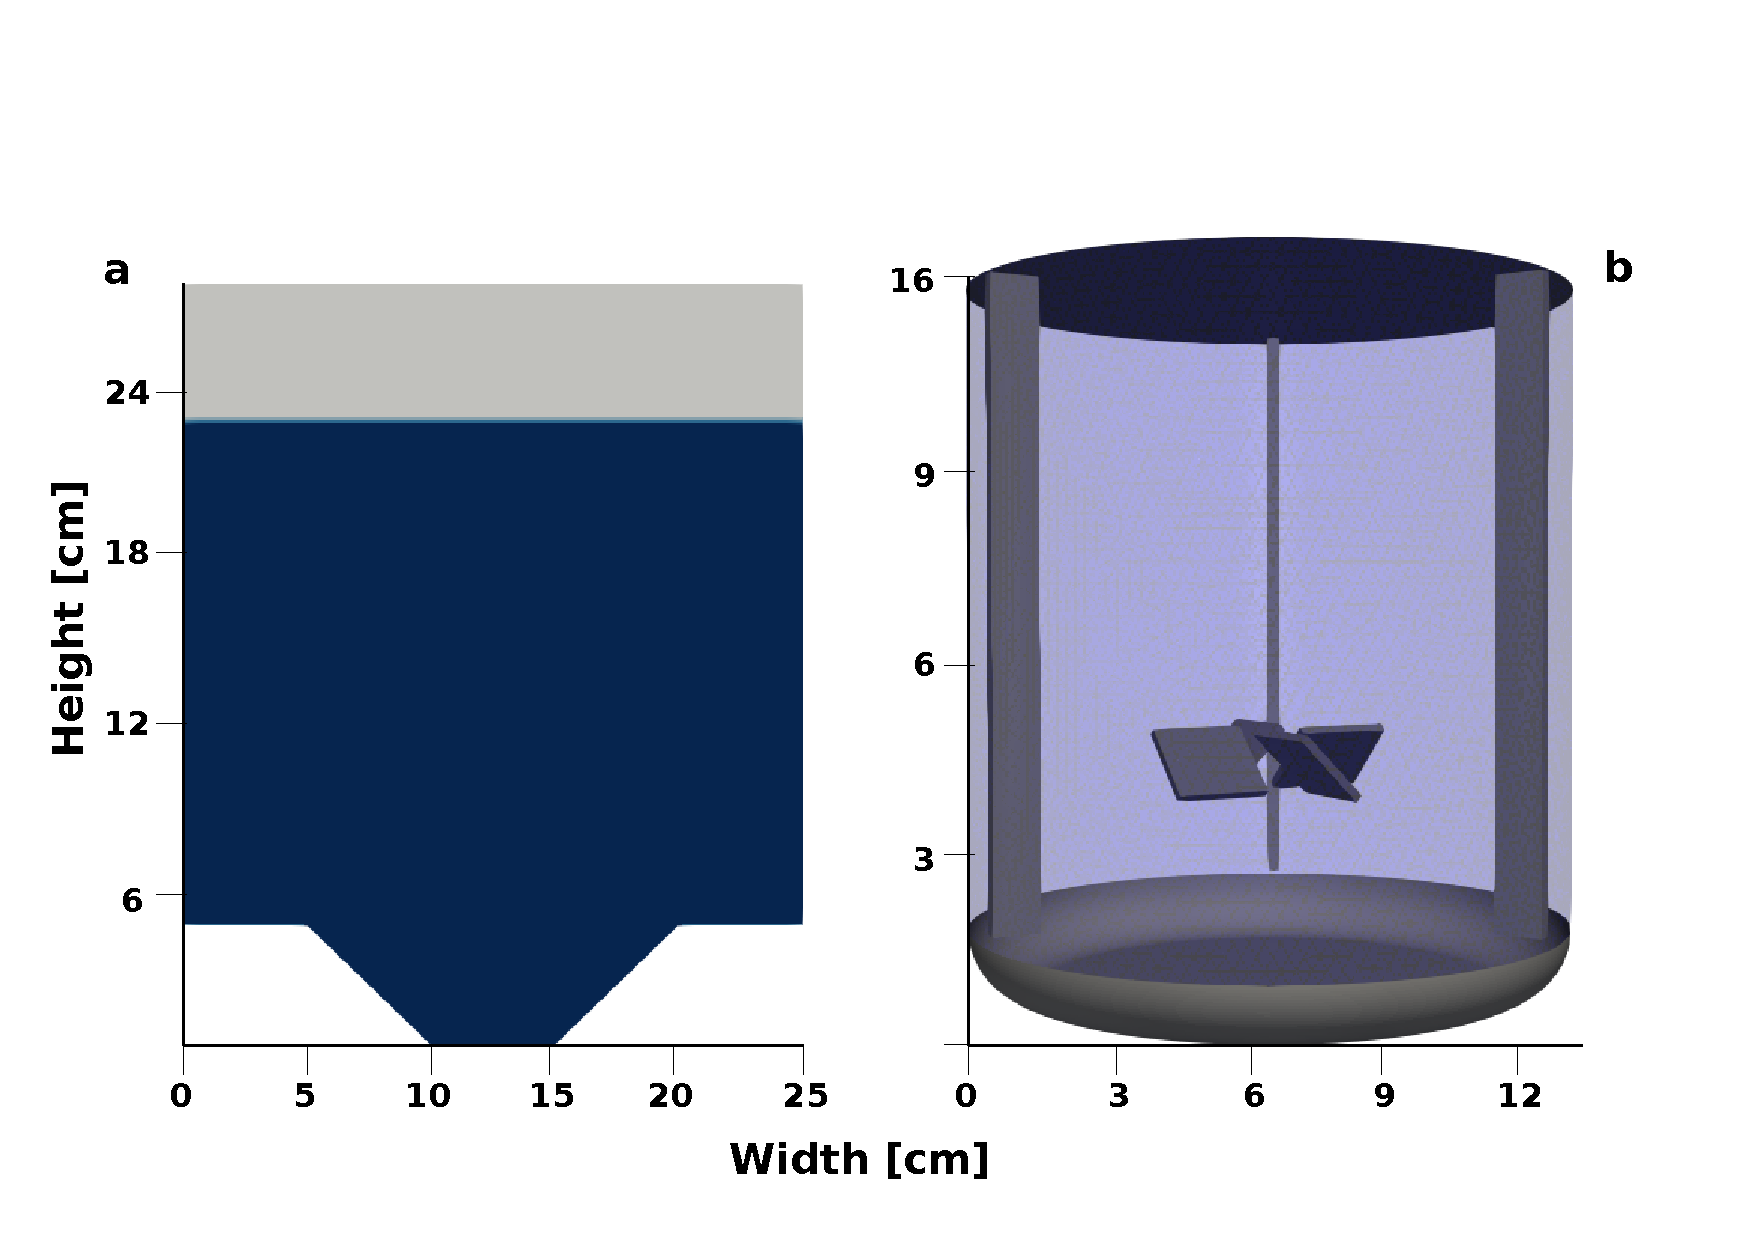
\includegraphics[width=1\linewidth]{Images/Chap3/geoms.pdf}
\caption{Representation of the geometries of the FPR (a) and the CR (b) upon which the simulations were based. The depth of the FPR is 6.0 cm. The blue region of the FPR represents the initial liquid volume fraction in the reactor, with the grey region representing the headspace. A single liquid phase was simulated in the case of the CR.}
\label{fig:geoms}
\end{figure}

Both geometries were developed in the CAD package Salom\'{e} M\'{e}ca \cite{electricitedefrance1989}. The surfaces were meshed as 2-dimensional triangular meshes. A fine triangular surface mesh ($\mathtt{\sim}$ 1 million discrete surfaces) was applied such that the geometries were watertight (\emph{i.e} there were no gaps in the tesselated surfaces) when used in the meshing process. The resulting meshes were exported as stereolithographic files as a basis for the volume meshes. Meshing was done using the \texttt{cartesianMesh} application, a hexehedral dominant meshing utility belonging to the \texttt{cfMesh} library \cite{creativefields2015} which is built upon the OpenFOAM framework \cite{theopenfoamfoundation2017}. The meshes are presented in the supplementary material (S.1).

\subsection{Fluid flow}
\label{ssec:flow}

\subsubsection{Governing equations}

It is assumed that the flow consist of an incompressible, Newtonian fluid under steady-state, isothermal conditions. The flow is considered to be turbulent and is modelled using the Reynolds-Averaged Navier-Stokes (RANS) equations with an appropriate turbulence model. The RANS equations are derived by decomposing the fluctuating velocity and pressure fields into their time-average plus an instantaneous fluctuation from the mean, i.e.

\begin{align}
\mathbf{u}(\mathbf{x}, t) &= \mathbf{U}(\mathbf{x}) + \mathbf{u}^\prime(\mathbf{x}, t)
\end{align}
%
and 
%
\begin{align}
p(\mathbf{x}, t) &= P(\mathbf{x}) + p^\prime(\mathbf{x}, t)
\end{align}
%
where $\mathbf{u}$ and $p$ are the instantaneous velocity and pressure fields; $\mathbf{U}$ and $P$ are the time-averaged velocity and pressure fields; and $\mathbf{u}^\prime$ and $p^\prime$ are the instantaneous fluctuations in velocity and pressure from the mean.

For an incompressible fluid, the Reynolds-averaged conservation of mass equation is expressed as

\begin{align}
\nabla \cdot \mathbf{U} &= 0
\end{align}

The RANS equations for the steady-state conservation of momentum is expressed as 

\begin{align}
\nabla \cdot (\mathbf{UU}) &= \left(\nu + \nu_T\right) \nabla ^2 \mathbf{U} - \frac{1}{\rho} \nabla P 
\end{align}
% 
where $\nu$ is the kinematic viscosity and $\rho$ is the density of the fluid, which remain fixed for the cases considered in this study. The turbulent (eddy) viscosity, $\nu_T$ results from the velocity fluctuations and represents the increased diffusivity due to turbulent mixing. Most often, two-equation turbulence models are used to determine the eddy viscosity, since they give a reasonable balance between accuracy and computational cost \cite{versteeg1995}.
\skippingparagraph
The eddy viscosity is defined through the Boussinesq hypothesis, given as 

\begin{align}
-\overline{u_i^\prime u_j^\prime}
&= \nu_T \left(\frac{\partial U_i}{\partial x_j} + \frac{\partial U_j}{\partial x_i} \right) - %\frac{2}{3}k\delta_{ij}
\end{align}

where the overbar represents a time-average, $k$ is the turbulent kinetic energy, and $\delta_{ij}$ is the Kronecker delta function. In practice, the eddy viscosity is defined by the solution of turbulence model equations. Most often, two-equation turbulence models are used, which give a reasonable balance between accuracy and computational cost \cite{versteeg1995}. 
\skippingparagraph
In this work, the $k-\omega$ SST model of \cite{menter1994} is used. This model implements a blending between a $k-\omega$ formulation in the near-wall region and a $k-\epsilon$ formulation in the free-stream region. This avoids the need for damping functions near the wall that are required for $k-\epsilon$ models and avoids problems with sensitivity to free-stream conditions that occur with standard $k-\omega$ models.
\skippingparagraph
The governing equation for the turbulent kinetic energy, $k$, is as follows \cite{menter1994}

\begin{align}
\frac{\partial k}{\partial t} + \mathbf{U}  \cdot \nabla  k &= \tilde{P_k} - \beta^*k\omega + \nabla \cdot \left[(\nu + \sigma_k \nu_T)\nabla k \right]
\label{eq:k}
\end{align}
%
where $\beta^*$ and $\sigma_k$ are constants, $\tilde{P_k}$ is the production rate of turbulent kinetic energy (with a production limiter applied to prevent build up in stagnation regions), and $\omega$ is the specific dissipation rate. The dissipation date is calculated in the $k-\omega$ SST model using the following transport equation \cite{menter1994}

\begin{align}
\frac{\partial \omega}{\partial t} + \mathbf{U} \cdot \nabla \omega &= \alpha S^2 - \beta \omega ^2 + \nabla \cdot \left[(\nu + \sigma_\omega \nu_T ) \nabla \omega  \right] \nonumber \\ 
&+ 2 (1 - F_1) \sigma_{\omega 2} \frac{1}{\omega} \nabla k \cdot \nabla \omega)
\label{eq:omega}
\end{align}
%
where $\alpha$, $\beta$, $\sigma_\omega$, and $\sigma_{\omega 2}$ are constants, $S$ is the invariant of the strain rate tensor, and $F_1$ is a blending function.
\skippingparagraph
With the solutions of Eqs.\ \ref{eq:k} and \ref{eq:omega}, the eddy viscosity is then calculated according to

\begin{align}
\nu_T = \frac{a_1 k}{\text{max}(a_1\omega, SF_2)}
\end{align}
%
where $a_1$ is a constant and $F_2$ is a blending function \cite{menter1994}. Values of all constants and auxiliary functions can be found in the work of Menter, 1994 \cite{menter1994}.
\skippingparagraph
The RANS equations also require wall functions to specify the near wall velocity when the viscous sublayer is not fully resolved by the mesh. The wall functions here implement a blending of viscous and log-law profiles, such that they are robust to mesh refinement, which is an important factor in separating discretisation and modelling errors \cite{menter2003}.

\subsubsection{Hydrodynamic boundary and initial conditions}

The initial conditions for the hydrodynamic model were zero gauge pressure and zero velocity at all points within the domains. At all walls, no-slip velocity boundary conditions were applied, along with zero gradient pressure conditions. When gradient conditions are applied at all walls, the pressure level must be set at some point within the domain. This is done internally in OpenFOAM by setting the gauge pressure to zero in a single (arbitrary) control volume. For the CR, a flow field was induced using four impeller blades pitched at 45\degree, spinning at 130 RPM. For the FPR, gas with the physical properties of nitrogen entered the domain at a rate of 6 L/minute through the inlet patches. 

%%%%%%%%%%%%%%%%%%%%%%%%%%%%%%%%%%%%%%%%%%%%%%%%%%%%%%%%%%%%%
% RADIATIVE TRANSPORT GOVERNING EQUATIONS
%%%%%%%%%%%%%%%%%%%%%%%%%%%%%%%%%%%%%%%%%%%%%%%%%%%%%%%%%%%%%
\subsection{Radiative transport}
\subsubsection{Governing equations}
Radiation delivery remains one of the major process bottlenecks to the design and effective operation of photobioreactors. There are many PBR CFD studies which treat the radiative field as a Beer-Lambert approximation, however this approach does not account for in-scattering phenomena. Failure to incorporate in-scattering in the CFD solution can lead to errors of as much as 20\% \cite{berberoglu2007}. The general form of the radiative transfer equation (RTE) accounts for the in-scattering effects, and is defined as

\begin{align}
\frac{dI_\lambda (\mathbf{r}, \mathbf{s}) }{ds} &=  \kappa_{\lambda}I_{b\lambda} \, - \, (\kappa_\lambda + \sigma_{\lambda, s}) \ I_\lambda (\mathbf{r}, \mathbf{s}) \nonumber \\
&+ \frac{\sigma_{\lambda, s}}{4 \pi} \int_{4 \pi} I_\lambda (\mathbf{r}, \mathbf{s'}) \Phi_\lambda(\mathbf{s}, \mathbf{s'}) d\Omega'
\label{eq:RTE}
\end{align}


\noindent where $I_\lambda$ is the spectral radiation intensity for wavelength $\lambda$, $\mathbf{r}$ is the position vector, $d\Omega$ is a differential solid angle that is centred along the vector $\mathbf{s}$, $s$ is the distance along $\mathbf{s}$, $\kappa_\lambda$ is the spectral absorption coefficient, and $\sigma_{\lambda,s}$ is the spectral scattering coefficient. The first term on the right accounts for black-body radiation. As we are accounting for either solar or artificial optical radiation, and relatively low temperatures of operation ranging between 4 \degree C and 40 \degree C, this term has been omitted from the solution. The second term on the right hand side accounts for absorption and scattering,  which combine to create the extinction term. For each participating species within the liquid phase, we can include an extinction term, which sum to that shown in Eq.\ \ref{eq:RTE}. The third term accounts for in-scattering through the phase function $\Phi_\lambda$. 
\skippingparagraph
There are several phase functions which have proven useful for photosynthetic media conditions: Henyey-Greenstein (HG) \cite{kong2014}, truncated phase function (TPF) \cite{berberoglu2007}, and the Schlick model (SM) \cite{jarosz2008}. \cite{jarosz2008} found that in the field of computer graphics and animations, the Schlick model was less computationally expensive but was still able to approximate the effects of anisotropic scatterings to the same standard as the HG model. The Schlick model is defined as;

\begin{equation}
\label{eq:schlick}
\Phi_s(k, \theta) = \frac{1 \, -\,  k^2}{4\pi (1\, +\,k\, cos(\theta))^2 }
\end{equation}
%
where $k \, \in [-1;1]$ and $\theta \, \in [0;\pi]$. The parameter $k$ implies an average cosine of scattered angles with a positive value giving preference to forward-scattering, a negative value giving rise to back-scattering, and a null value denoting isotropic scattering. The angle $\theta$ is the scattering angle of a ray.
\skippingparagraph

The implementation of the RTE in the form of Eq.\ \ref{eq:RTE} does not translate readily to photobioreactors, where multiple multiple participating species may exist, with different extinction coefficients. The expression has therefore been modified to include the participating species within a photosynthetic medium along with their specific absorption and scattering coefficients, which have been combined into a global spectral extinction coefficient ($E_j$) associated with each participating species $X_j$. The modified RTE, with the black-body radiation term omitted, is given as

\begin{equation}
\label{eq:rteSimplified}
\frac{dI_\lambda (\textbf{r}, \textbf{s})}{ds} \, = \, - \sum_{j} [E_{\lambda,j} X_j] I_\lambda (\textbf{r}, \textbf{s}) \,+\, \frac{\sigma_{\lambda, s, j}}{4 \pi} \int_{4 \pi} I_\lambda (\textbf{r}, \textbf{s}^\prime) \Phi_\lambda(\textbf{s}, \textbf{s}^\prime) d\Omega^\prime
\end{equation}


Custom software libraries, given the name \texttt{photoBio}, were written in order to extend or replace parts of the existing radiation libraries in OpenFOAM to suit the purpose of this study. As an example, in the standard OpenFOAM implementation, the radiative field is specified by temperature boundary conditions, while the irradiance can be specified directly in the customised solver.  Another novelty in the custom \texttt{photoBio} library was that models needed to accept all participating media as input. The absorption and scattering expressions were therefore extended to allow for any number of species in a mixed-culture multiband system as shown in Eq.\ \ref{eq:rteSimplified}. Finally, the scope for the inclusion of phase scattering functions was adapted from previously built libraries of \cite{kong2014}. The Schlick model was added to this list of functionality, and was used for the cases shown in this study.
\skippingparagraph
The particular method used for the resolution of the radiative field was the finite volume discrete ordinates method (fvDOM), renamed to \texttt{photoBioDOM} in the custom libraries that were written. The fvDOM is the conservative formulation of the discrete ordinates method \cite{raithby1990}, which allows the solution method to be implemented within the same finite volume framework as the flow and biokinetics models.


\subsubsection{Radiative transfer boundary conditions and parameters}

An incident irradiance of $30\, Wm^{-2}$ was applied to the outer walls of both the CR and FPR. A single wavelength band of peak $850\, \pm 5 nm$ was used for this simulation. Other important parameters governing the fvDOM angular discretisation and the biomass coupling were used in this simulation and are summarised in Table \ref{tab:photoBioProperties}.

\begin{table}[tp]
\caption{FvDOM and biomass coupling parameters for the radiation component of the solution procedure}
\centering
\label{tab:photoBioProperties}
\begin{tabular}{p{2.5cm} p{1.2cm}  p{2.3cm} p{4.5cm} p{1.3cm}}

\hline
\textbf{Quantity} & \textbf{Value} & \textbf{Units} & \textbf{Meaning} & \textbf{Ref.}\\ \hline
$n_\phi$ & 6 & - &azimuthal angle discretisation & - \\ \\
$n_\theta$ & 6 & - & polar angle discretisation & - \\ \\
$n_{p,\phi}$& 3 & - & overhanging control azimuthal angle pixelation & - \\ \\
$n_{p,\theta}$& 3 & - & overhanging control polar angle pixelation & -\\ \\
$k$ & 0.98 & - & Forward/back scattering Schlick asymmetry factor & \cite{jarosz2008}, \cite{berberoglu2007a}\\ \\ 
$a_{X_{PB}}$ & 106 & $m^2 kgCOD^{-1}$ & absorption for a given \textit{Rb. sphaeroides} (COD) biomass concentration at $850\, nm$ & \cite{berberoglu2007a}\\ \\
$\sigma_{X_{i}}$ & 19 & $m^2 kgVS^{-1}$ & scattering for a given \textit{Rb. sphaeroides} (COD), $X_S$, and $X_I$ biomass & \cite{berberoglu2007a}\\
\hline
\end{tabular}
\end{table}
\newpage
\subsection{Biokinetic model}
Biokinetics were taken from a lumped parameter model \cite{puyol2017}. This considers growth of biomass and consumption of $COD$, $NH_4N$, and $PO_4P$ but does not consider photon delivery. The state space includes three particulate state variables, PPB biomass, particulate composite biomass, and inert solids, as well as seven soluble state variables. All of these are represented as scalar differential variables. The governing equations for the solid and soluble state variables ($\phi_i$) subject to advection, diffusion, and generation or consumption are as follows.

\begin{align}
\frac{\partial \phi}{\partial t} + \nabla \cdot \left( \mathbf{U}\phi \right) - \nabla^2 D_\phi \phi = r_{\phi}
\end{align}

\noindent where $\mathbf{U}$ is the frozen velocity field of the fluid phase, ${D}_{\phi}$ is the diffusivity coefficient of scalar $\phi$ in water, and $r_{\phi}$ represents the generation or consumption terms, as previously defined in \cite{puyol2017}. The diffusivity of the solid species was set to $10^{-11} \mathrm{m^2 s^{-1}}$ for stability purposes.
\skippingparagraph
The term $r_\phi$ for each state variables includes a Monod term ($\zeta_I$) with respect to irradiance (I) at any point in space (Eq. \eqref{eq:monodG850}). This means that the radiative field, and the biokinetic expressions have an interdependence which must be considered in the solution procedure.

\begin{align}
\label{eq:monodG850}
\zeta_I = \frac{I}{K_I + I}
\end{align}

\subsubsection{Biokinetic boundary conditions and parameters}
Each scalar quantity in the biokinetic model was set to a uniform initial value. Zero-flux boundary conditions were specified for each wall in the domain for all state variables. Initial conditions are presented in the supplementary material (S.2).

\subsection{Solution procedure}
\label{ssec:soln}
The solution procedure shows the order in which the governing equations are solved (Fig.\ \ref{fig:solnHierarchy}). The momentum equations are solved until a quasi steady-state is found. This approach is applicable to both the single phase and multiphase systems. Secondly, for the multiphase system, the velocities for each phase are segregated. The single phase CR is not modified at this stage. Finally, the initial conditions for the biochemical equations are set, the radiative field is solved, and the biochemical equations are solved. The radiative field is updated every 15 minutes of simulation time.

\begin{figure}[tp]
\centering
\includegraphics[width=0.6\linewidth]{Images/Chap3/algo_devt.pdf}
\caption{Solution algorithm for the solver. Momentum equations are solved until steady state is achieved and fed to the biochemical equation solver. The radiative field is updated every 15 minutes of simulated time.}
\label{fig:solnHierarchy}
\end{figure}

The flow field is solved first. The assumption that the solid species do not participate in the flow field can be made for PBRs which have relatively low total suspended solids concentrations compared with other activated sludge processes \cite{bitog2011}. The solver then enters a coupled radiation-biokinetics loop in which the radiative field is updated every 15 minutes of simulated time. A solution procedure that updated the radiative field at every time step was tested, but was prohibitively slow, and it was found to be unnecessary to update at such high frequency. Since the change in radiative properties due to biomass growth occur over an extended time frame, the update interval was found to not substantially influence the results.
\skippingparagraph

The solver used for these simulations is the \texttt{pamFoam} solver: a multiphase, multiphysics implementation of a finite volume hydrodynamics, radiation, and biokinetics solver, which is built upon version 5.0 of the OpenFOAM framework, a collection of C++ libraries for solving continuum mechanics problems \cite{theopenfoamfoundation2017}. The solver and run-time dictionaries have been released under the AGPL-3 license, and can be accessed online (https://gitlab.com/leboucher/pamFoam/tags/v5.1.0). The solver incorporates a custom radiation transport library built upon the finite volume discrete ordinates method \cite{raithby1990}, but adapted for use with phototrophic models. Its source code can also be found online (https://gitlab.com/leboucher/photoBio/tags/v5.1.0). The solid and soluble species were implemented as passive scalar transport equations.


%%%%%% RESULTS AND DISCUSSION

\section{Results and Discussion}
%The differences in characteristic time constants between enzymatic response ($10^{-6}\, s$), dynamic radiative field ($10\, s$) and microbial growth (hours or days) are multiple orders of magnitude. Therefore, when analysing PBR systems, the evolution of the radiative field due to microbial growth (order of hours), the dynamic radiative field (order of seconds), need to be considered. As the time scale of enzymatic response is low when compared to the other two phenomena, the associated effects do not require analysis. 

\subsection{Radiative field dynamics}

As the biomass grows in suspension over time, There is a decrease in intensity and distribution of the radiative field (Cf Eq. \ref{eq:rteSimplified}). This is shown in Fig.\ \ref{fig:rad_evol}(a). This demonstrates that despite a similar radiation intensity, the geometry of the FPR is better than the CR, resulting in a higher average irradiation intensity, and a greater attenuation over time due to faster biomass growth. Fig.\ \ref{fig:rad_evol} also shows spatial distribution of radiative intensity at the start of the simulation, and at 24 hours. Sub-figures b and c correspond to the FPR, and sub-figures d and e show the CR. This demonstrates a substantial attenuation over time from 12 $\mathrm{W m^{-2}}$ to 7 $\mathrm{W m^{-2}}$ in the FPR and from 5 $\mathrm{W m^{-2}}$ to 3 $\mathrm{W m^{-2}}$ in the CR. The percentage decrease corresponded to an increase in the phototrophic biomass $\mathrm{X_{PB}}$ from $\mathrm{0.5 \, g\, COD\, L^{-1}}$ to $\mathrm{1.0 \, g\, COD\, L^{-1}}$ in the FPR and $\mathrm{0.5 \, g\, COD\, L^{-1}}$ to $\mathrm{0.8 \, g\, COD\, L^{-1}}$ in the CR over the same period of 24 hours. The change in other particulate species was relatively small over that same time period. 

\begin{figure}[tp]
\centering
\includegraphics[scale=0.75]{Images/Chap3/rad_field_dynamics.pdf}
\caption{Evolution of the radiative field ($\mathrm{W m^{-2}}$), volume averaged over all time steps, and the spatial changes over time for the FPR and CR. Cross-sectional view at reactor from 0 cm to 3 cm from the radiation source. (b,c) corresponds to the radiative field at the start of the simulation, and (d,e) is the radiative field at 24 hours for the FPR and CR respectively.}
\label{fig:rad_evol}
\end{figure}

Findings from other studies \cite{kong2014} have shown that volumes within a reactor with an irradiance below $\mathrm{2\, Wm^{-2}}$ are effectively dark zones. Over time, self shading by biomass becomes apparent, which means that the fluid hydrodynamics become increasingly important if PBRs are to maintain substantial phototrophic biomass at high concentrations. For the FPR, the volume percentage of dark zones is 0\%, compared with 30\% for the CR. At 24 hours of simulated time, despite  25\% more particulate matter, only 25\% of the volume is in the dark, compared with 55\% for the CR. Both the limitations in nutrient and photon availability mean that this proportion sees diminishing rates of biomass shading as the simulation continues. These results support other findings that in suspended biomass PBRs, the majority of the reactor is in the dark when operating at steady state with substantial phototrophic biomass and particulate concentrations. It is clear that for near infrared radiation, attenuation is more significant within the phototrophic media than in the gas phase, and both multiphase (gas-liquid) and single phase liquid systems were modelled, although a more thorough investigation around the bubble dynamics and their effect on the radiative field is required to quantify these interactions.

\subsection{Short-term particle radiation dynamics}
\label{ssec:strf}
The short term particle radiation dynamics result from the fluid field moving biomass particles within the heterogeneous radiative field as shown in Fig. \ref{fig:G850_short}. The first column (a,c) corresponds to the particle radiation dynamics of the FPR, with the same data being represented as a dynamic plot (a) and a frequency histogram (c). The second shows the parallel results for the CR. This demonstrates that biomass in both reactors is subject to on-off irradiance cycles on the order of 3-5 s, with an amplitude of 20 $\mathrm{W m^{-2}}$. However, the dynamics are quite different, with particles in the FPR being irradiated for longer, and with a higher base-line (5 $\mathrm{W m^{-2}}$ in the FPR compared with 0 $\mathrm{W m^{-2}}$ in the CR). This indicates that in the FPR, particles are effectively always irradiated at a minimum level, whereas in the CR,  there is complete on-off cycling. 

\begin{figure}[tp]
\centering
%\hspace*{-2cm} 
\includegraphics[width=1.\linewidth]{Images/Chap3/G850_short.pdf}
\caption{Particle radiation dynamics for an 850 nm band of irradiance. The top row (a, b) shows the transient radiative field experienced by a PPB particle for the FPR and CR reactors respectively. The same field is represented for both reactors (c, d) as a histogram on the bottom row. Both reactors have an incident irradiance of 30 $\mathrm{ W m^{-2}}$.}
\label{fig:G850_short}
\end{figure}

A question arising of the dynamic radiative field is whether the PPB biomass is sufficiently fast to respond to these changes. If the biomass response is much faster than the change in intensity, the growth kinetics can be treated as a continuous function (with dependence on intensity). If biomass response kinetics are also on the order of seconds, lower-level expressions would be required (which also consider photo-enzyme kinetics). The response time for \textit{Rhodobacter sphaeroides} was determined in the literature to be in the order of $10^{-11}$ seconds \cite{slouf2012}; a time constant much smaller than the periods seen in Fig. \ref{fig:G850_short}. Therefore, this justifies the use of a continuous function with respect to radiation for both this case, and in scaled-up systems, since they will generally have longer time constants due to the larger dimension with respect to velocity. This also justifies the approach used in this study to generate results, with biomass growth coupled to the radiative field, and phototrophic organisms self-shading as they grow.

\subsection{Growth of PPB biomass and uptake of soluble substrates}
\label{ssec:ppb_growth}
Four comparative simulations were done to assess the full Eulerian solution (as used so far in this study - solution 4) to three reduced continuously stirred tank reactor (CSTR) versions. These include (for each reactor):

\begin{enumerate}
    \item Uniform irradiance at incident value $\mathrm{30.0\, W\, m^{-2}}$ (ODE1). This is the standard approach that can be applied in a lumped-parameter model \cite{bechet2013}.
    \item Irradiance fixed at the the volume-averaged value as presented at in Fig. \ref{fig:rad_evol}(a). These values for the FPR and CR were $\mathrm{11\, W\, m^{-2}}$ and $\mathrm{5\, W\, m^{-2}}$ respectively (ODE2).
    \item Dynamic irradiance as determined and presented in Fig. \ref{fig:G850_short}(a, b). This data is treated as a dynamic input to the lumped parameter model (ODE3). The main reduction in extent compared to a full CFD simulation is that the biomass/substrate do not need to be represented by scalars. In order to represent the effect of only modelling the liquid-irradiance system, the 30 s profile was replicated in time to 24 h rather than taking the full dynamic profile which includes long-term temporal light attenuation due to biomass growth.
    \item Full Eulerian CFD solution (CFD).
\end{enumerate}

In the first two cases, no CFD is required, while in the latter two cases, CFD is required to identify the particle radiation exposure pattern, and for the integrated model respectively. The first two cases were explored because certain studies have taken modelling approaches using lumped parameters based on single values of uniform irradiance, with little information as to the spatial distribution of the radiative intensity field. This has been applied using either the surface incident exposure \cite{uyar2007, zhou2014}, or volume averaged irradiance \cite{molinagrima1996, bordel2009}. This can lead to an over-prediction when reporting growth rates.
\skippingparagraph
The biomass concentrations (in mgCOD/L) are shown for the various modelling approaches for both systems (Fig. \ref{fig:growth_evol}(a, b)). These demonstrate light-limited, fairly uniform growth rates towards the substrate depletion point where the growth stops (\textit{i.e.} a batch system). The uniform irradiance approaches generally over-predicted growth rates, particularly in the cylindrical reactor (where irradiation was fundamentally less efficient). The dynamic exposure approach was generally effective in representing biomass profiles, but with a clear deviation with respect to the full CFD approach. Specifically, there were slightly slower growth rates for ODE3 vs CFD. This is somewhat surprising since the final attenuation is higher in the full CFD approach when compared with ODE3 (due to biomass growth), but could be explained by the fact that this attenuation is due to biomass exposure rather than water attenuation. Therefore the light is not "lost", but rather used during attenuation.
\skippingparagraph
Fig. \ref{fig:growth_evol}(c-f) shows the uptake concentration of soluble substrates of the same simulations. Again, the hybrid approach (ODE3) is most effective compared with CFD, but there are substantial deviations for all three ODE approaches. The large deviations for substrate $\mathrm{S_{AC}}$ (Fig. \ref{fig:growth_evol}(c, e)) and $\mathrm{S_S}$ (Fig. \ref{fig:growth_evol}(d, f)) are most likely caused by inhibition of each respective uptake process (photoheterotrophic uptake for acetic acid, and for other organics) caused by the presence of the other soluble compound class. This, combined with the difference in uptake rates for acetate uptake ($\mathrm{2.4\, d^{-1}}$) and photoheterotrophic uptake ($\mathrm{1.4\, d^{-1}}$) \cite{puyol2017} mean that based on the amount of light available in the system, different behaviour can occur.  
\skippingparagraph
The full ODE approach (ODE1, ODE2), as stated above, is the most common approach, taking either surface irradiation \cite{uyar2007, zhou2014}, or an approximated reduced average irradiance \cite{lee1987, molinagrima1996, bordel2009}. This provided unsatisfactory results, particularly in the simplified CR. With respect to growth rates, and in an actual system, these variations would be absorbed by biochemical parameters, making them non-transferable to other systems. A system can only be effectively approximated with a lumped parameter modelling approach if the reactor is not only well mixed, but also well serviced with a uniform irradiance which can be measured effectively. This would likely not be an effective photobioreactor field design, but these factors also mean that some care must be taken even in laboratory systems when determining biological parameters, since the surface measured irradiance will almost certainly not be the \textit{in situ} irradiance. This would have an impact on apparent biomass growth parameters. 
\skippingparagraph

\begin{figure}[ht]
\hspace*{-0.75cm}
\includegraphics[scale=0.5]{Images/Chap3/growth_kinetics.pdf}
\caption{Biomass growth and substrate uptake for the FPR (a, c, e) and the CR (b, d, f). The first row shows the growth of PPB and the second and third rows show the consumption of acetic acid and other readily biodegradable soluble organics respectively. For all figures, the triangles correspond to ODE1, the diamonds correspond to ODE2, the the crosses represent ODE3, and the solid line is the CFD solution.}
\label{fig:growth_evol}
\end{figure}

The dynamic irradiance approach (ODE3) was far more effective in biological simulation, but the irradiance profile changes in each case, and cannot effectively represent irradiance changes as biomass experiences long-term growth. This has quite complex impacts, including potentially a loss in efficiency due to reduced biomass based attenuation. When compared with the full Eulerian solution (CFD), the dynamic irradiance solution has a slightly slower growth rate, but the time constant is similar for both simulations. The hybrid approach therefore has some value, particularly where a full model cannot be formulated. However, the full model provides complete interpretation at a modest increase in computational complexity. 

\subsection{Limitations of the model}
\label{ssec:limitations}
\subsubsection{CFD considerations}
There are three main limitations of the study with respect to the CFD implementation. Firstly, while gas and liquid phases have been modelled and biochemical state variables have been segregated in the liquid phase, the effect of biological activity on the gas field have not been incorporated. The mass transfer between phases was also not considered in this case. Including mass transfer models is important for photoautotrophic (gas fed) or photosynthetic ($\mathrm{CO_2}$) growth. Any mass transfer model is dependent on how the dispersed gas field is solved. Here, a uniform bubble Eulerian approach was taken, but an alternative that considers bubble size distribution such as population balance modelling could lead to an improvement in prediction of mass transfer. A better represented bubble size distribution would also allow analysis of its dynamic effects on the radiative field.  
This model considers planktonic biomass modelled as passive scalars. The momentum coupling would not substantially change interaction with the radiative field. However, an important possible extension is the inclusion of a spatially explicit biofilm. The current model lends itself well to include a continuum based biofilm model as a module in a broader continuum-based phototrophic growth model. 
\skippingparagraph
As the biomass has been implemented as passive scalars, the effects of changes in biomass concentration on the flow fields have not been quantified (\textit{i.e.}, does not affect rheology, density or momentum). This could be incorporated through an upgrade of the biomass from scalar to dispersed phase. Modelling the solid system in a Lagrangian framework can also link the particulate species with a set of physical information, such as particle density and diameter. The particulate species as they are currently modelled could also be linked to a particulate density, which would then have an effect on the flow field. 

\subsubsection{Biochemical system limitations}
This system differs from photosynthetic algae or cyanobacteria, where photosynthetic organisms may be in multiple states (excited, photoinhibited or resting) \cite{bechet2013}. The state depends on the radiative intensity and the light history of the organisms. In addition, nitrogen storage becomes an important factor \cite{bernard2011}. The short-term particle radiation dynamics as observed here are even more important in photosynthetic systems, where the transition in biological state adds another system dynamic which is on the same speed order as the cycling speed. Therefore, consideration of photo-dynamics is even more important when simulating white light systems, since, as discussed above, enzyme response is extremely fast (and photo-dynamics do not interact with this), while a change in photo-state is far slower. Photo-inhibition is another important factor not considered in the current model. The current system was irradiated with 30 $\mathrm{W m^{-2}}$, and photo-inhibition has been reported to start occurring closer to 900 $\mathrm{W m^{-2}}$ \cite{miyake1999}. Updating the model to include photo-inhibition terms would increase the range of applicability of the model to outdoor PBR systems, and is an important factor for white light systems as discussed above. The time constant for recovery from photo-inhibition may make this a more complex response function, and increase the importance of considering photo-dynamics. 
\skippingparagraph
This model was simulated looking at a single radiation band at 850 nm. In reality, the growth of PPB depends on other wavelength bands, including 375 nm and 590 nm (facultative carotenoids) and the near infrared band ranges from 830 nm to 900 nm \cite{overmann2013}. Upgrading the biochemical model to include the growth on several different wavelengths would lead to resolution of important aspects, including increased and differential attenuation of higher energy radiation. However, assigning fixed behaviour to organisms which can adapt to different environmental conditions, such as the growth or loss of chromaphores due to low or high intensity radiative fields, means that there will always be a level of uncertainty which cannot be described by the model. 

%%%% Conclusions
\section{Conclusions}
This study has looked at two different reactor setups; a flat plate reactor (FPR) and a cylindrical reactor (CR). Over these two different reactor geometries, four modelling approaches were evaluated;
\begin{enumerate}
    \item ODE1: An ODE system taking a uniform radiative field equal to that of the incident irradiance.
    \item ODE2: An ODE system taking a uniform radiative field equal to its value halfway into the domain as solved by the radiative transfer equation here, or alternatively by a Beer-Lambert relationship.
    \item ODE3: An ODE system taking as input a dynamic irradiance experienced by a particle as it is carried by the velocity field in the reactors.
    \item CFD: A full Eulerian CFD approach accounting for fluid flows, radiative transfer, and the system of biochemical equations for purple phototrophic bacteria.
\end{enumerate}

The first two approaches tended to over-predict growth rates, meaning that the spatial variations within PBRs are important to consider, and local effects can have an impact on the overall solution. The results for ODE3 were similar to those for the full Eulerian CFD solution, irrespective of reactor geometry. This approach presents an appropriate compromise when computational resources are scarce, however the full Eulerian approach provides the complete interpretation for the PBR systems, with scope to expand on this model with more physical processes. 
\skippingparagraph
Several limitations to the study were identified, and were classed in two categories; CFD limitations and biochemical modelling limitations. The CFD limitations were that mass transfer in multiphase systems was not solved, and the model was developed as a planktonic model with passive scalars, limiting the description of physical processes such as biofilm development and effects on the flow field due to changes in density. The biochemical limitations extended on previous work to highlight the adaptive changes of pigment production in response to the radiative field, and the effects of photoinhibition on uptake rates.
%CFD including photo-attenuation identified that particles were subject to both short and long-term irradiative dynamics, the former due to cycling through light-dark regions, and the latter due to overall biomass growth. A biologically coupled CFD solution versus uniform irradiance ODE approaches (as commonly applied) found the latter could not effectively predict dynamics of growth in batch. A compromise (which identified particle irradiation dynamics from non-coupled CFD) was effective, but the computational effort approached the full CFD method.

%\section*{Acknowledgements}
%The authors would like to thank Domenico Santoro and the team at Trojan Technologies, London, Canada, for their help with CFD simulations for photobiological systems. This work was funded by the CRC for Water Sensitive Cities (project C2.1). Christopher De Groot acknowledges funding from the Natural Sciences and Engineering Research Council of Canada (NSERC) [RGPIN-2017-04078].

%\section*{Appendix. Supplementary material}
%Supplementary material has been provided with this work \\(DOI: 10.6084/m9.figshare.7459106.v2). In addition, the model codes can be found at https://gitlab.com/leboucher/pamFoam/tags/v5.1.0 for the solver, and https://gitlab.com/leboucher/photoBio/tags/v5.1.0 for the \texttt{photoBio} library. 


% *************** CHAPTER 4 ***************
\cleartoevenpage
\pagestyle{empty}	%Use this to suppress the header from the preceding chapter.


\begin{table}[h]
	\begin{center}
	\begin{tabular}{|c|l|l|}
		\hline
		Contributor & Statement of contribution & \% \\
		\hline
		\textbf{Edward M. Barry}	    & writing of text 			& 80\\
										& proof-reading				& 60 \\
										& theoretical derivations 	& 50 \\
										& numerical calculations 	& 100\\
										& preparation of figures 	& 100 \\
										& initial concept			& 30 \\
		\hline
		Christopher T. DeGroot			& writing of text 			& 0\\
										& proof-reading				& 5 \\
										& supervision, guidance 	& 15\\
										& theoretical derivations 	& 10\\
										& preparation of figures 	& 0 \\
										& initial concept			& 0 \\
		\hline
		Shakil Ahmmed       			& writing of text 			& 10\\
										& proof-reading				& 0 \\
										& supervision, guidance 	& 25\\
										& theoretical derivations 	& 40\\
										& preparation of figures 	& 0 \\
										& initial concept			& 0 \\
		\hline
		Tim H\"{u}lsen		    		& writing of text 			& 0 \\
										& proof-reading				& 0 \\
										& supervision, guidance 	& 10 \\
										& theoretical derivations 	& 0 \\
										& preparation of figures 	& 0 \\
										& initial concept			& 35 \\
		\hline
		Damien J. Batstone	    		& writing of text 			& 10\\
										& proof-reading				& 95 \\
										& supervision, guidance 	& 50 \\
										& theoretical derivations 	& 0 \\
										& preparation of figures 	& 0 \\
										& initial concept			& 35 \\
		\hline
	\end{tabular}
	\end{center}
\end{table}


%-------------------------------------------------------------------------------------------------------%
%-------------------------------------------------------------------------------------------------------%
%-------------------------------------------------------------------------------------------------------%
%-------------------------------------------------------------------------------------------------------%
%-------------------------------------------------------------------------------------------------------%
%-------------------------------------------------------------------------------------------------------%
%This is an internal chapter of the thesis.
%If you have a long title, you can supply an abbreviated version to print in the Table of Contents using the optional argument to the \chapter command.
\chapter[A multidimensional phototrophic biofilm model]{A multidimensional, phototrophic, continuum-based biofilm model}
\label{chap:ch4}	%CREATE YOUR OWN LABEL.
\pagestyle{headings}

\section*{Abstract}
Phototrophic bacteria have an ability to remove soluble organics and nutrients from waste streams while at the same time producing products of high value such as pigments, biocrude, high protein feedstock. 
However, phototrophic and photosynthetic systems are critically dependent on light delivery and biomass harvesting to remove organics and nutrients from the process.
No substantial work to date has been done on modelling photo-dependent biofilm growth.
This study aims to develop a multidimensional continuum-based phototrophic biofilm model to serve as a basis for exploring the physical mechanisms associated with photobiofilm formation and for potential process optimisation. 
A volume of fluid (VoF) model in which phototrophic biomass could be grown on a substratum was developed. 
This evaluates the interactive mechanisms of substrate transport and radiative attenuation through the bulk and biofilm. 
Investigating coupling between the biofilm and the radiative field was the major motivator of the study. 
The lamp source was set from below and above the biofilm on both uniformly and sparsely initiated biofilms at 30 W m\textsuperscript{-2}. An extra simulation was done where the lamp source was set at 10\% intensity and placed below the biofilm. In all cases, there was phototrophic growth, however in the case of minimal irradiation, the maximum growth rate was 70\% slower than the case with 30 W m\textsuperscript{-2}. 
Maximum growth rate was 25\%-30\% slower in the cases where the radiative intensity field was initiated from above the biofilm, due to liquid attenuation. This was despite the decreasing substrate diffusion limitations. 

%This model provides a basis for a multispecies, multidimensional phototrophic biofilm model which accounts for all physical phenomena in the life-cycle of the biofilm, however experimental work is required to calibrate the model for a non-planktonic case.
%-------------------------------------------------------------------------------------------------------%
%-------------------------------------------------------------------------------------------------------%
%-------------------------------------------------------------------------------------------------------%
\section{Introduction}
Despite a growing interest in the use of purple phototrophic bacteria (PPB) for wastewater treatment and the production of high valued products, there remain key engineering challenges which render widespread adoption in full scale installations unfeasible at this moment.
The major challenges have already been discussed throughout this thesis, but to reiterate, light delivery, the additional requirement of bioavailable organics, and solid-liquid separation are some of the major barriers \cite{hulsen2016}. 
Process modelling is an important tool for a better understanding of how phototrophic processes work, and for eventual process design and optimisation. 
Indeed, this thesis is based on the modelling of these phototrophic processes using the distributed parameter approach of computational fluid dynamics (CFD). 
This work has built upon the development of a biokinetic model, where the main metabolic processes were defined in a manner that ensured compatibility with the International Water Association family of models (IWA) such as the anaerobic digestion model 1 (ADM1) \cite{batstone2002} or the ASM models \cite{henze2000}. 
The biokinetic process model was extended to include dynamics in multidimensional space in order to demonstrate the spatially varying nature of the radiative field, and by extension, the growth of phototrophic biomass. 
In addition to organics and radiative field limitations, the third constraining factor is the separation of the solid phototrophic biomass from the liquid phase. 
Previously, anaerobic membrane bioreactors were proposed as a solution for solid-liquid separation at laboratory-scale implementations \cite{hulsen2016}, however with increased capital and operational expenditure when compared to conventional wastewater treatment processes, more separation techniques need to be explored. 
Growing biomass attached to walls as biofilm can be a method to reduce harvesting costs of phototrophic biomass, as well as reducing inefficient delivery of light due to the self shading associated with biomass growth. As such, a phototrophic biofilm model in a CFD framework needs to be developed. 
\skippingparagraph
Phototrophic biofilms are communities of phototrophic biomass, other organisms, and other organic and inorganic substances such as extra-cellular polymeric substances \cite{vanloosdrecht2002}. 
Much work has been dedicated to understanding the behaviour of biofilms in order to limit the harm they cause, such as in medical settings, sewer networks \cite{pikaar2014}, and in membrane separation processes, commonly referred to as fouling \cite{radaei2018}. Biofilm formation can also be favoured and encouraged depending on the application. 
Trickling filters are an example of beneficial biofilms which consist of wastes being sprayed over fixed granular beds. Thick biofilms develop therein and remove pollutants and toxicants from the filter's biofilm \cite{donlan2002}. Other examples of beneficial biofilms include the bioremediation of contaminated soils \cite{singh2006}, which claim an advantage over biological treatment with planktonic cells in that microorganisms in biofilms are more resilient to extreme conditions, and therefore have a better chance at adapting to their particular environment. Biofilms may grow on a physical substrate (moving or fixed media), or be self supporting in the form of anaerobic or aerobic granules \cite{baeten2018}. 
\skippingparagraph
In order to successfully model biofilm formation and behaviour, the governing processes need to be identified. The major processes are the initial attachment, biofilm growth, biofilm decay, and detachment \cite{alpkvist2007}. 
These processes have been represented by several modelling approaches. The approaches are divided into first, second and third generation models as defined by the IWA task group on biofilm modelling \cite{wanner2006}. 
The progress from first to third generation has seen the modelling approach evolving from mass transfer to the inclusion of complex microbial interactions and an update to two and three dimensional descriptions. First generation models involved the description of substrate gradients (mostly a single limiting substrate) within an homogeneous 1-dimensional zone of biomass. Second generation models differed from their predecessors in that they included multiple substrates and microorganisms in a heterogeneous distribution. They were still limited to a 1-dimensional description. 
Third generation models represent particulates as discrete elements, a continuum field, or a combination of both. Discrete biofilm models include cellular automata and agent based models \cite{skoneczny2015}. 
With discrete techniques, cells are subjected to a set of rules that govern their behaviour in terms of attachment, substrate uptake and cell division, and decay and detachment processes \cite{skoneczny2015}. 
These models are relatively simple to develop, however simulation cycles require statistical rigour and multiple simulation runs, as the aggregate effect of individual particles can result in artefacts, which need to be assessed by averaging multiple runs (or very large numbers of discrete elements) \cite{dacunto2017}. 
In contrast to discrete third generation biofilm models, continuum-based models involve a full spatio-temporal and mechanistic description of biofilm processes \cite{eberl2001}. 
An advantage of continuum-based biofilm models over discrete approaches is that a mechanistic description of growth processes can be developed into the model.
Biokinetic models such as the Eilers-Peeters model for algal growth \cite{eilers1988} or the PAnM1 model \cite{puyol2017} can therefore be used directly within a phototrophic biofilm modelling framework, albeit with some manipulations to convert the model from a COD or equivalent basis, to a volumetric growth basis. 
\skippingparagraph
Despite the increasing interest in phototrophic bioreactors, and the motivation to better control photobiofilm development, there are only two clear examples of phototrophic biofilm modelling. 
The first continuum-based biofilm model \cite{clarelli2013} identified the non-conservative nature of interface evolution tracking methods such as the level-set method \cite{alpkvist2007} and proposed a mixture model for cyanobacterial biofilms. 
The mixture model treats each point in space as an information holder, in which multiple physical properties and states can exist. 
This mixture model provided a mathematical description of a specific case of a cyanobacterial biofilm which according to the authors could be extended to all phototrophic biofilm systems. 
This study presented an exponential decay function for the radiative field through the biofilm, which has a tendency to under predict the radiative distribution for optically thick media such as biofilms \cite{jarosz2008}. 
In optically thick media, strong scattering effects are observed, including forward scattering \cite{jarosz2008}. 
This phototrophic/photosynthetic biofilm mixture model was further developed in subsequent studies \cite{polizzi2017}. In this study a single functional microbial group (microalgae), its associated carbon pool, and an extra-cellular polymeric matrix were all defined as biofilm components. CO\textsubscript{2}, O\textsubscript{2} and inorganic nitrogen formed the liquid component of the model. Mass transfer between phases was updated to include diffusion terms, and biofilm expansion was expressed in terms of biological mechanisms such as photosynthesis, cell maintenance, EPS excretion and cell decay. 
The radiative field was also modelled as an exponential decay function in terms of path length and the concentrations of participating biofilm components.
\skippingparagraph

The proposed model in this work differs from the previous PBF examples in the following aspects:

\begin{enumerate}
\item Biofilm models should be developed for implementation in all spatial dimensions. Decisions to simplify the model should be made by the user at implementation. Presented here is a multidimensional phototrophic biofilm model.
\item The evolving structure of the biofilm must be captured. The advancement of the biofilm front is coupled to biomass growth and decay processes. The interface between biofilm and liquid is captured by a conservative, coupled volume-of-fluid (VoF) and level-set method.
\item Biofilms are heterogeneous in nature. Scope must be made to model multispecies biofilm evolution. As such, presented here is a multidimensional,  multispecies, dynamically structured phototrophic biofilm model.
\end{enumerate}

In addition to these three points of novelty, the biofilm model has been implemented in OpenFOAM, a computational fluid dynamics (CFD) finite volume method (FVM) framework. This package is a collection of C++ libraries which allow for the resolution of continuum mechanics problems. The model extends on previous work by the authors \cite{puyol2017}. The global purpose of this study is to explain the physical phenomena occurring within biofilms so that subsequent studies can progress the work for design or prediction purposes.

This study therefore aims to extend the previous work done on the development of a lumped parameter model in chapter 2, and of a phototrophic CFD model in which a coupled photo-biological radiative transfer model and planktonic growth model were defined in chapter 3. A combination of the volume of fluid (VoF) and mixture methods are used in this work: the VoF method to segregate the biofilm from the liquid phase, and the mixture method within the biofilm to differentiate between active phototrophic biomass (PPB  in this case), biodegradable particulates (X\textsubscript{S}) and inert particulates (X\textsubscript{I}). This method allows for conservation to be maintained while more accurately capturing the interface between the liquid and biofilm phases. 


%As biofilms are spatially heterogeneous structures, both spatial and temporal variations must be considered in order to describe the physical phenomena. Biofilm models can be divided into three main classes: \textit{i)} one-dimensional models capable of including mass transfer, reaction/diffusion, and detachment processes \cite{horn2014}, \textit{ii)} multidimensional discrete biofilm models such as cellular automata and agent based methods \cite{wang2010}, and \textit{iii)} continuum models including computational fluid dynamics (CFD) approaches \cite{alpkvist2007, duddu2009, cunault2015}. Despite the vast suite of modelling approaches and examples existing within the literature, there have been few studies which defining biofilm behaviour in phototrophic systems, where the spatially varying nature of the radiative field could be an important factor in the heterogeneous formation of biofilms. \\

%Representing biomass as continua can be advantageous. Firstly, the currency of process engineering modelling is differential balance equations. Continuum modelling is therefore a common language for communication of model development and results, and additionally, conservation of differential states can be ensured. In contrast to discrete modelling methods, deterministic solutions can be obtained for continuum-based models \cite{dacunto2017}. Difficulties can arise when modelling continuum-based biofilms. The frequently abrupt density jumps across liquid/solid boundaries can lead to numerical instabilities. The coupling of the non-linear transport equations with growth kinetics can also be problematic. Additionally, solving state equations with vastly different time constants (and order of 10s of seconds for fluid flow in a reactor, to hours or days for biomass growth and decay expressions) can make the resolution of the time discretisation difficult. Differential algebraic equations, or appropriate time discretion algorithms for stiff systems of differential equations can overcome this barrier. Computational fluid dynamics (CFD) packages can assist with some of the numerical problems and the mathematical formulation difficulties associated with continuum models.


% \begin{itemize}
% \item Biofilms are communities of microorganisms, EPS matrices and inert substances living together
% \item There are extrinsic properties leading to their growth:
% \begin{itemize}
% \item fluid flows
% \item irradiance
% \item presence of nutrients
% \item presence or absence of other microorganisms
% \item shear rates
% \item reactor geometry and operating conditions (implicitly)
% \end{itemize}
% \end{itemize}

%%%% PROBLEM DESCRIPTION
%\newpage
%\section{Problem description}
%\label{S:problem_description}
%The modelling approach is concerned with the description of a phototrophic biofilm system consisting of purple phototrophic bacteria (PPB). The model description for this system has been previously described \cite{puyol2017}, however this did not account for spatial variations, and by extension, biofilm formation was not considered. The phototrophic biofilm grows attached to a surface substratum. Above the biofilm is a body of nutrient-rich liquid. Incident photons of wavelength 850 \si{\nano \metre} are irradiated from either \si{\Gamma_0} or \si{\Gamma_3} into the domain \si{\Omega}, as shown in Fig. \ref{fig:2d_above}. The initial thickness of the biofilm is \SI{50}{\micro \metre} with uniformly distributed solid species. The factor of incident irradiance is also explored, with three different irradiance levels of \SI{10}{\watt \metre ^2}, \SI{30}{\watt \metre ^2}, and \SI{100}{\watt \metre ^2} being simulated from the surface substratum. Incident irradiance in all cases is assumed uniform and diffuse across the whole boundary.


% The phototrophic biofilm (PBF) model based on purple phototrophic bacteria is an extension of the models presented previously \cite{puyol2017} (\textbf{include my model}). Biofilm treatment extends work previously carried out by \cite{alpkvist2007}, \cite{alpkvist2007}. The important physical processes identified are as follows:
% \begin{itemize}
%     \item Coupled volume of fluid and level set for capturing of the biofilm/liquid interface.
%     \item Radiative transfer coupled to the growth of the biokinetics.
%     \item Biokinetics equations coupled to the radiative transfer equation (RTE) and the biofilm advection terms.
%     \item Development of a biofilm front velocity based on the evolution of pressure due to solid species growth within the biofilm.
% \end{itemize}


%\begin{figure}[htpb]
%    \centering
%    \includegraphics[scale=0.5]{Images/Chap4/prob_diagram_below.pdf}
%    \caption{Two-dimensional representation of the simulation domain for the case of a bottom-irradiated biofilm. Boundaries \si{\Gamma_4} and \si{\Gamma_5} are out of, and into the page respectively, and take the same boundary conditions as boundaries \si{\Gamma_1} and \si{\Gamma_2}. The irradiance source (\si{h \nu}) is in fact uniform and diffuse across the whole boundary. Subscripts relating to \si{\alpha}, namely \textbf{l} and \textbf{B} correspond to liquid phase fraction, and biofilm phase fraction respectively.} 
%    \label{fig:2d_above}
%\end{figure}


%%%%%%%%%%%%% MATHEMATICAL FORMULATION

\newpage
\section{Mathematical formulation}
\label{S:formulation}
\subsection{Radiative transfer}
The general form of the radiative transfer equation (RTE) has been adapted to phototrophic systems, presented in the previous chapter and adapted from an earlier implementation \cite{kong2014}. 
It includes the dependency on the concentration of solid species and water. 
The black body radiation term has been omitted from this equation due to its minimal influence. 
The electromagnetic field energy balance is presented in Eq. \eqref{eq:rteSimplifiedCh4}. 

\begin{equation}
\frac{dI_\lambda (\textbf{r}, \textbf{s})}{ds} \, = \, - \sum_{j} [E_{\lambda,j} X_j] I_\lambda (\textbf{r}, \textbf{s})\, +\, \frac{\sigma_{\lambda, s, j}}{4 \pi} \int_{4 \pi} I_\lambda (\textbf{r}, \textbf{s}^\prime) \phi_\lambda(\textbf{s}, \textbf{s}^\prime) d\Omega^\prime
\label{eq:rteSimplifiedCh4}
    \end{equation}

where $I_\lambda$ is the spectral irradiance for a given wavelength, \textbf{r} is the position vector of a radiative ray, \textbf{s} is the direction vector of the ray, and s is the path length. The first term on the right hand side is the extinction term, with $E_{\lambda, j}$ being the specific extinction coefficient (the combination of scattering and absorption components) for participating species $X_j$. The second term on the right hand side is associated with in-scattering, where $\sigma_{\lambda, s, j}$ is the scattering coefficient, and $\Phi_\lambda$ is the wavelength scattering function from path \textbf{s} to scattered direction $\textbf{s}^\prime$ through solid angle $d\Omega$. The phase scattering function, $\Phi_\lambda$ for this model is the Schlick function (Eq. \ref{eq:schlick}), which is appropriate for optically thick media \cite{jarosz2008}. 

\begin{equation}
\Phi_s(k, \theta) = \frac{1 \, -\,  k^2}{4\pi (1\, +\,k\, cos(\theta))^2 }
\end{equation}

where parameter $k$ takes values between -1.0 and 1.0 included, with negative or positive values corresponding to back-scattering and forward scattering respectively. A value of 0 means scattering is isotropic. The parameter $k$ represents the average cosine of the scattered angles. The angle $\theta$ is that between the previous path and scattered path of a ray.

\subsection{Consumption and release of soluble substrates}
Soluble substrates exist in both the volume of liquid, and the porous part of the biofilm volume. Growth and release expressions (hydrolysis of biodegradable particulate organic matter) have been previously described \cite{puyol2017}. The soluble substrates considered in this study are readily biodegradable soluble organics expressed in chemical oxygen demand (COD), acetic acid (COD), hydrogen (COD), inorganic carbon (C), inorganic nitrogen (N), inorganic phosphorus (P) and soluble inert material (COD). The general form for the soluble balance equation is expressed in Eq. \ref{eq:solublesD}.

\begin{equation}
\label{eq:solublesD}
\frac{\partial S_{\phi}}{\partial t} + \nabla (\mathbf{U} S_{\phi}) - \nabla \cdot (D_{\phi} \nabla S_{\phi}) = \Gamma_{\phi}, 
\end{equation}

where, S is the soluble species and ${\phi}$ = SI, SH${_2}$, SIC, SAC, SIN, SIP and SS. ${D_{\phi}}$, and ${\Gamma_{\phi}}$ are the diffusivity, and growth rate of species ${\phi}$, respectively. The units in which the soluble species are expressed are the same as in previous chapters, that is, kg\{COD, N, P\} m\textsuperscript{-3}, depending on the soluble component. 


\subsection{Growth of particulate matter}
The previously defined equations, Eq. \eqref{eq:solublesD}, express their respective uptakes and growth in terms of COD. 
This representation is valid for the soluble state variables if we assume that they do not directly contribute to the phase fractions. 
However, particulate species must be expressed in terms of volume fractions, $\alpha_{XPB}$, $\alpha_{XS}$ and $\alpha_{XI}$. 
This can be achieved by introducing a conversion term $\rho^*$ which is similar to the assumption in previous studies where its value was assumed to be roughly 60-70 kg TS m\textsuperscript{-3} \cite{alpkvist2007,polizzi2017}. 
In this case, we have taken a more systematic approach in converting the COD quantities of the particulate species to volume fractions. 
Let $\rho^*_{C\alpha}$ be the term which links the COD to the volume fraction $\alpha$ of the particulate of interest. The values for biofilm bulk density ($\rho_{BF}$), cell water fraction (w\textsubscript{C}), biofilm porosity ($\epsilon_{BF}$, and particulate COD:VS ratio ($\kappa_{CV}$) need to be specified. Biofilm bulk density and cell water fraction values were sourced from literature \cite{zhangBishop1994} as 1010 kg m\textsuperscript{-3} and 90\% respectively for PPB. For the other particulates, the cell water fractions were assumed to be less, as these particulates are not living and do not require water for maintenance processes. Their water fraction was therefore assumed to be 83\%. The biofilm void fraction was expressed by a linear relationship in terms of biofilm bulk density, which for a bulk density of 1010 kg m\textsuperscript{-3}, gave a void fraction ($\epsilon$) of 0.56. Eq. \eqref{eq:void_frac} shows this relationship which is linear for densities between 1000 kg m\textsuperscript{-3} and 1100 kg m\textsuperscript{-3} \cite{humeng2013}. 
\begin{equation}
    \label{eq:void_frac}
    \epsilon \, = \, 8.16 - \num{0.0075}\rho_{BF}
\end{equation}
To convert COD content to VS, the values were sourced from previous studies, where the COD:VS ratio for PPB was assumed to be 1.78 kgCOD/kgVS \cite{puyol2017} and those for particulates X\textsubscript{I} and X\textsubscript{S} were assumed to be that of glucose at 1.07 kgCOD/kgVS. The expression to convert from COD to volume fraction is therefore as defined in Eq. \eqref{eq:cod2alpha}

\begin{equation}
    \label{eq:cod2alpha}
    \rho^*_{C\alpha} \, = \, \rho_{BF} \cdot \kappa_{CV} \cdot (1.0 - \epsilon_{BF}) \cdot (1.0 - w_C)
\end{equation}

For all particulates in the system, the conversion factor remained constant at 80 kgCOD m\textsuperscript{-3}, however the variation of any of these components could be varied for sensitivity analysis. This value was about 15\% greater than that proposed in previous photobiofilm studies \cite{polizzi2017}, and remains a source of uncertainty which could be resolved with experiments, which have been well discussed in the literature \cite{azeredo2017}. 

\skippingparagraph
The growth of particulate matter increases the mass of the biofilm and influences the pressure equation which induces advection of the biofilm front. The particulate species included in this study are PPB, slowly biodegradable particulate organics, and inert particulate organic matter. Similarly to \cite{alpkvist2007}, $X_i$, the concentration of particulate species $i$ is expressed by $\rho^*\theta_i$ where $\rho^*$ is the density of particulate species, assumed constant for each species, and $\theta_i$ is the volume fraction of species $i$. The growth terms for the particulate balance equations (Eq.~\ref{eq:particulate}) have been previously defined \cite{puyol2017}.


\begin{equation}
\label{eq:particulate}
\frac{\partial \alpha_{\phi}}{\partial t} + \nabla (\mathbf{U} \alpha_{\phi}) - \nabla \cdot (D_{\phi} \nabla \alpha_{\phi}) = \frac{\Gamma_{\phi}}{\rho^*_{C\alpha}}, 
\end{equation}

where $\alpha$ is the volume fraction of the particulate species and ${\phi}$ = \{XPB, XS and XI\}. The diffusivities for soluble species in both the bulk and biofilm were sourced from literature \cite{stewart2003, stewart1998}. For the particulate species, an artificial diffusion constant was used in the Laplacian term such that spurious diffusion of solids across the biofilm/liquid interface did not occur. This approach has also been applied in the literature \cite{haroun2010}. The diffusivity of particulates in the bulk phase was set arbitrarily low such that no solid species could exist there. Within the biofilm, the diffusivity was set to \num{0.000000000089} m\textsuperscript{2}s\textsuperscript{-1}, representing the cell motility within the biofilm structure \cite{ali2018}.  

\subsection{Hydrodynamics}
\label{Hydro}
The multiphase volume of fluid (VoF) flow may be calculated using the mixture mass, momentum and continuity equations as follows,

\begin{equation}
    \label{eq:continuity}
    \nabla \cdot \mathbf{U} = \Gamma,
\end{equation}

\begin{equation}
    \label{eq:mass}
    \frac{\partial \alpha_w}{\partial t} + \nabla\cdot (\phi \alpha_w) = \dot{m},
\end{equation}

\begin{equation}
    \label{eq:momentum}
    \frac{\partial (\rho \mathbf{U})}{\partial t} + \nabla\cdot (\rho \mathbf{U U}) = -\nabla P + \rho \mathbf{g} +\nabla \cdot (\vec{\tau}+\vec{\tau}_t)+f_{\sigma},
\end{equation}
where, $\mathbf{U}$ is the velocity, $\Gamma$ is the growth term, $\alpha_w$ is the phase fraction of the water, ${\phi}$ is the mass flux, ${\dot{m}}$ is the mass transfer, ${\rho}$ is the density, \textbf{g} is the gravitational acceleration, P is the pressure, $\vec{\tau}$ is the viscous stress, $\vec{\tau_t}$ is the turbulent stress, and ${f_{\sigma}}$ is the surface tension force. The mixture density is expressed as:

\begin{equation}
    \label{eq:mixtureDensity}
    \rho = \rho_w \alpha_w + \rho_b (1-\alpha_w),
\end{equation}
where, ${\rho_w}$ and ${\rho_b}$ are the densities of the water and biofilm phases respectively. The surface tension force ${f_{\sigma}}$ may be calculated as follows,
\begin{equation}
    \label{eq:surfaceTension}
    f_{\sigma} = \sigma k \nabla\alpha_w.
\end{equation}
Here, ${\sigma}$, and $k$ are the surface tension coefficient, and curvature, respectively. The curvature $k$ may be written as, 

\begin{equation}
    \label{eq:curvature}
    k = -\nabla \mathbf{n} = -\nabla \Bigg(\frac{\nabla \alpha_w}{\big| \nabla \alpha_w\big|} \Bigg),
\end{equation}
where, \textbf{n} is the outward unit normal vector at the interface.


\section{Applications}
\subsection{Boundary and initial conditions}
A series of five scenarios were simulated in order to highlight the important aspects of the model. These are summarised in Table \ref{tab:biofilm_cases}. These cases were selected because previous studies had noted that radiation delivery was one of the major limitations to reactor performance in a suspended growth context \cite{hulsen2016, hulsen2016a}. The rationale was that simulations exploring these limitations would aid in understanding the dynamics of phototrophic biofilm growth. In the base cases, the radiative intensity was delivered from below an assumed transparent substratum. The second case considered a limiting case of irradiance at 10\% of that reported in the literature \cite{hulsen2018}. Additionally, the baseline experiment was modified such that the radiative field was initialised from above the biofilm. The last two simulations considered sparsely initiated biofilm with the radiative field being initialised from below and above the biofilm (summarised in Table \ref{tab:biofilm_cases}). 

\begin{table}[H]
    \centering
    \small
    \renewcommand{\arraystretch}{1.4}
    \caption{Suite of differing operating conditions for the biofilm simulations for both 2D and 3D cases.}
    \tabcolsep=0.11cm
    \begin{tabular}{@{}p{2cm} p{4cm} p{5cm} p{5.5cm}@{}} \toprule
Case & Irradiance  &  \{$\alpha$\textsubscript{XPB\textsubscript{0}}, $\alpha$\textsubscript{S\textsubscript{0}}, $\alpha$\textsubscript{I\textsubscript{0}}\}  &  Configuration \\ \hline
1    &  30 Wm\textsuperscript{-2}   &  \{0.7, 0.0, 0.2\}$\mathbb{1}^*_{y<0.03\mathrm{mm}}$  & Incident below\\
%2     &  80 Wm\textsuperscript{-2}  &  \{0.7, 0.0, 0.2\}$\mathbb{1}_{y<0.03\mathrm{mm}}$ & Incident below\\
2    &  5 Wm\textsuperscript{-2}  &    \{0.7, 0.0, 0.2\}$\mathbb{1}_{y<0.03\mathrm{mm}}$  & Incident below\\
3    &  30 Wm\textsuperscript{-2}  &   \{0.7, 0.0, 0.2\}$\mathbb{1}_{y<0.03\mathrm{mm}}$  & Incident above\\
4    &  30 Wm\textsuperscript{-2}  &   \{0.7, 0.0, 0.2\}  & Sparse biofilm, incident below\\
5    &  30 Wm\textsuperscript{-2}  &   \{0.7, 0.0, 0.2\}  & Sparse biofilm, incident above\\ \hline
    \end{tabular}
  \scriptsize{* $\mathbb{1}$ is the characteristic function where the stated initial biofilm concentration applies if the condition is true, or is zero if false.} 
    \label{tab:biofilm_cases}
\end{table}

For all other state variables, initial and boundary conditions were maintained constant across all simulations.\\

In the case of boundary conditions, the velocity field was treated as the no-slip at the boundaries whereas the fixed-flux-pressure was imposed for the pressure field. Conversely, in the case of phase fractions, i.e. ${\alpha}$, the inlet-outlet boundary condition, which is a mixture of zero-gradient and fixed-value boundary conditions, is considered at the outlet, and the walls are treated as zero-gradient. The boundary conditions may be summarised on all boundaries as,  

\begin{equation}
    \label{eq:boundaryU}
    U_x = U_y = U_z = 0,
\end{equation}

\begin{equation}
    \label{eq:boundaryPrgh}
    \nabla P_{rgh} = \bigg[\frac{\phi \frac{H(\mathbf{U})}{a_p} - \phi}{|S_f|a_p} \bigg],
\end{equation}

\begin{equation}
    \label{eq:boundaryAlpha}
    \frac{\partial \alpha}{\partial \mathbf{n}} = 0 \quad {and} \quad \alpha = \alpha_i.
\end{equation}
Here, ${P_{rgh}}$ is the pressure excluding the hydrostatic head, and H(\textbf{U}), ${a_P}$, ${\phi}$, and ${S_f}$ are the transported coefficients, matrix coefficients related to the variables, such as \textbf{U}, flux, and surface area vectors, respectively, of the discretised governing equations; n = x = y = z, and ${\alpha_i}$ is the internal cell centre value close to the boundary face. The initial conditions for the velocity and pressure fields are set zero. The volume phase fractions are initialised by defining the values for $\alpha_{{XPB}}$, $\alpha_{{XS}}$, $\alpha_{{XS}}$, and $\alpha_{{w}}$. The volume fractions were set such that their sum was unity for all cells within the domain. 

\subsection{CFD workflow}
The model was developed using OpenFOAM 6 from the OpenFOAM Foundation \cite{openfoamfoundationltd2017}. The solver was adapted from the \texttt{interFoam} and the \texttt{pamFoam} solvers. The new solver was named \texttt{photoBiofilmFoam}. As this study has been concerned with the coupling of biofilm growth, delivery of substrate, and the radiative field, no flow fields were included as their inclusion would have presented some numerical difficulties, detracting from the analysis of the physics of interest. After the initial biofilm was set, the volume fraction of liquid was solved. The growth of biomass was used as a source term for the phase volume fraction of the biofilm field (to satisfy the volume of fluid governing equations). After the growth of biofilm and the changes in phase fractions were calculated, the radiative field was solved at an interval of 300 s. After the biochemical, phase fraction, and radiative transfer equations were solved, the momentum equations were corrected. The time step was governed by the Courant-Friedrich-Lewy condition and was maintained below 0.5 for the entirety of the simulation. A mesh Independence study was  carried out over the orders of \num{10000}, \num{100000}, and \num{1000000} cells, and 160 000 cells were where the solution converged. 

%%%%%%%%%%%%%%%%% Implementation
\section{Results}

\subsection{Case 1: Uniformly initiated biofilm irradiated from substratum}
% ! DO Biomass first
% ! DO distributions second
% ! DO Growth rates last
Case 1 has been treated as the base case for the simulations. The irradiance was initiated below the sustratum, and the biofilm was initiated as a uniform layer on the substratum with values as per Table \ref{tab:biofilm_cases}. Figures \ref{fig:case1_ppb_frac}, \ref{fig:case1_growth_frac} and \ref{fig:case1_dist_frac} show the volume fraction of PPB, its apparent growth rate, and the spatial distribution of particulates and water at four points in time: 1.0 d, 4.0 d, 7.0 d, and 10.0 d. 
\begin{figure}[H]
    \centering
     \hspace*{-1cm}\includegraphics[width=1.1\textwidth,height=0.4\textheight]{Chap4/methods/data/figures/case1_ppb_frac.png}
    \caption{Two dimensional view of PPB as uniformly initiated biofilm over a substratum irradiated at 30 W m\textsuperscript{-2} at 850 nm.} 
    \label{fig:case1_ppb_frac}
\end{figure}

Figure \ref{fig:case1_ppb_frac} shows the growth of PPB biomass at several steps in time. With soluble substrates in excess, PPB grows phototrophically from close to the substratum. New biomass effectively pushes the present biofilm away from the irradiated substratum, with uniformity in the biofilm composition governed by cell motility. In the absence of an external flow field, the biofilm continues to expand without shear stresses controlling any sloughing mechanism. Substrate is still able to be delivered to the highly irradiated regions, however this delivery rate decreases as the biofilm expands. 

\begin{figure}[H]
    \centering
     \hspace*{-1cm}\includegraphics[width=1.1\textwidth,height=0.4\textheight]{Chap4/methods/data/figures/case1_growth_frac.png}
    \caption{Two dimensional view of PPB growth rate as uniformly initiated biofilm over a substratum irradiated at 30 W m\textsuperscript{-2} at 850 nm.} 
    \label{fig:case1_growth_frac}
\end{figure}

Figure \ref{fig:case1_growth_frac} shows the apparent growth rate of PPB over time. There is a 33\% decrease in maximum growth rate over this period as diffusion begins to limit the growth and the initial water volume fraction begins to vacate the biofilm region as particulates start to dominate. Between 4.0 d and the end of the simulation, there is no longer any of the initial pore water in the biofilm domain, so the attenuation of the radiative field cannot explain the reduction in maximum apparent growth rate of PPB. However, the biofilm still includes water in the biofilm void space which doesn't change the apparent diffusivity for a zone of fully developed biofilm. This reduction in growth rate can be attributed to the reduction in delivery of substrate as the solubles need to diffuse through a thicker biofilm to reach the highly irradiated zone of the biofilm.

\begin{figure}[H]
    \centering
    \includegraphics[width=\textwidth,height=0.45\textheight]{Chap4/methods/output/case1.png}
    \caption{Spatial distribution of particulates and water over domain height. Biofilm was initiated as a uniform biofilm over a substratum irradiated at 30 W m\textsuperscript{-2} at 850 nm.} 
    \label{fig:case1_dist_frac}
\end{figure}
 
 Figure \ref{fig:case1_dist_frac} shows the distribution of particulate species along the height of the biofilm. In the absence of other heterotrophic biomass, the spatial distribution of the particulate species has minimal change. As PPB decays, it produces biodegradable particulates, and in turn, inert particulates. Over the period of 10 days, the biofilm front progresses to more than 12 times that of the initial biofilm level. As these cases have not included the shear stresses associated with an externally flowing field, nor the description of a set of detachment rules, the control of the biofilm front has not fully been specified. While this information is not central to this study, it could be included to provide a more complete picture of biofilm evolution in different environments.





\subsection{Case 2: Reduced substratum irradiance}
\begin{figure}[H]
    \centering
     \hspace*{-1cm}\includegraphics[width=1.1\textwidth,height=0.4\textheight]{Chap4/methods/data/figures/case3_ppb_frac.png}
    \caption{Two dimensional view of PPB as uniformly initiated biofilm over a substratum irradiated at 3 W m\textsuperscript{-2} at 850 nm.} 
    \label{fig:case3_ppb_frac}
\end{figure}

In the case of reduced irradiance from below the biofilm, the absolute growth of biofilm, as well as the apparent growth rate of biofilm are affected. The value of the applied irradiance is 3 W m\textsuperscript{-2} at 850 nm, which is much less than the half-saturation constant of 8.76 W m\textsuperscript{-2} at the same frequency \cite{eltsova2016}. The maximum apparent growth rate is 0.40 d\textsuperscript{-1}. The maximum growth rate stays constant throughout the simulation, most likely due to the low biofilm growth during this time, however we see in the latter stages of the simulation a clear instance of decay, where the irradiance is insufficient to sustain phototrophic activity, and the PPB that initially grew on the substratum begin to decay  as they are pushed further from the radiative field. We see through Fig. \ref{fig:case3_dist_frac} that the biofilm front increases threefold over the 10 day period. The proportion of other particulate matter increases slightly over this time period, and the volume fraction of PPB initially increases from 70\% to 75\%, but then steadies at 70\% as time progresses. 

\begin{figure}[H]
    \centering
     \hspace*{-1cm}\includegraphics[width=1.1\textwidth,height=0.4\textheight]{Chap4/methods/data/figures/case3_growth_frac.png}
    \caption{Two dimensional view of PPB growth rate as uniformly initiated biofilm over a substratum irradiated at 3 W m\textsuperscript{-2} at 850 nm.} 
    \label{fig:case3_growth_frac}
\end{figure}

\begin{figure}[H]
    \centering
    \includegraphics[width=\textwidth,height=0.45\textheight]{Chap4/methods/output/case3.png}
    \caption{Spatial distribution of particulates and water over domain height. Biofilm was initiated as a uniform biofilm over a substratum irradiated at 3 W m\textsuperscript{-2} at 850 nm.} 
    \label{fig:case3_dist_frac}
\end{figure}




\subsection{Case 3: Overhead irradiance}
\begin{figure}[H]
    \centering
     \hspace*{-1cm}\includegraphics[width=1.1\textwidth,height=0.4\textheight]{Chap4/methods/data/figures/case4_ppb_frac.png}
    \caption{Two dimensional view of PPB as uniformly initiated biofilm irradiated from above at 30 W m\textsuperscript{-2} at 850 nm.} 
    \label{fig:case4_ppb_frac}
\end{figure}

In this simulation, the radiative field was initialised from above the biofilm with an irradiance of 30 W m\textsuperscript{-2}. The biofilm does not reach the same level as that in Case 1, as the radiative field is partly attenuated before it reaches the biofilm. This means that growth is initially steady when compared to Case 1, but it accelerates the the biofilm forms and its front progresses. The initial apparent growth rate is 0.7 d\textsuperscript{-1} and this increases to 1.0 d\textsuperscript{-1} as the biofilm grows. With the in-scattered nature of the radiative field, the intensity is highest at the central point of the boundary. This is due to this point having the most number of neighbours potentially contributing to the radiative field. This results in the biofilm in the early stages of the simulation extending towards this point of highest irradiance. As the simulation progresses and growth is less limited by the irradiance, this biofilm shape becomes less pronounced.

\begin{figure}[H]
    \centering
     \hspace*{-1cm}\includegraphics[width=1.1\textwidth,height=0.4\textheight]{Chap4/methods/data/figures/case4_growth_frac.png}
    \caption{Two dimensional view of PPB growth rate as uniformly initiated biofilm irradiated from above at 30 W m\textsuperscript{-2} at 850 nm.} 
    \label{fig:case4_growth_frac}
\end{figure}

\begin{figure}[H]
    \centering
    \includegraphics[width=\textwidth,height=0.45\textheight]{Chap4/methods/output/case4.png}
    \caption{Spatial distribution of particulates and water over domain height. Biofilm was initiated as a uniform biofilm irradiated from above at 30 W m\textsuperscript{-2} at 850 nm.} 
    \label{fig:case4_dist_frac}
\end{figure}



\subsection{Case 4: Sparsely initialised biofilm with substratum irradiance}

Figures \ref{fig:case5_ppb_frac}, \ref{fig:case5_growth_frac} and \ref{fig:case5_dist_frac} show the biofilm front in terms of PPB, the distribution of the apparent growth rates for PPB and the spatial distribution of the biofilm components respectively. The system is initialised with 3 hemispherical (or cylindrical in 2 dimensions) zones of biofilm along the substratum. The two partial  spheres initialised in the corners begin at the origin and have a radius of 0.18 mm. The partial sphere initialised in the centre of the horizontal axis has a radius of 0.25 mm. 

\begin{figure}[H]
    \centering
     \hspace*{-1cm}\includegraphics[width=1.1\textwidth,height=0.4\textheight]{Chap4/methods/data/figures/case5_ppb_frac.png}
    \caption{Two dimensional view of PPB as sparsely initiated biofilm over a substratum irradiated at 30 W m\textsuperscript{-2} at 850 nm.} 
    \label{fig:case5_ppb_frac}
\end{figure}

Figure \ref{fig:case5_ppb_frac} depicts the biofilm structure as growth occurs over the 10 day period. With the radiative field being deployed from below the substratum, new biomass occupies the space in the region close to this field. Older biomass is pushed away from the substratum where the apparent growth rate tends to the decay rate. 

\begin{figure}[H]
    \centering
    \hspace*{-1cm}\includegraphics[width=1.1\textwidth,height=0.4\textheight]{Chap4/methods/data/figures/case5_growth_frac.png}
    \caption{Two dimensional view of PPB growth rate as sparsely initiated biofilm over a substratum irradiated at 30 W m\textsuperscript{-2} at 850 nm.} 
    \label{fig:case5_growth_frac}
\end{figure}

Figure \ref{fig:case5_growth_frac} demonstrates the growth of PPB, which effectively follows the intensity of the radiative field. The maximum apparent growth rate is constant at 1.4 d\textsuperscript{-1}. As the biofilm grows, the apparent growth rate diminishes, tending slightly negative where the radiative field is insufficient for phototrophic growth, or to zero for regions where there is no biomass in the domain. The apparent growth rate only becomes slightly negative in the region away from the substratum. The difference in attenuation coefficients (the sum of scattering and absorption coefficients) between the water phase and the biofilm phase is clearly demonstrated in the Fig. \ref{fig:case5_growth_frac} at 4.0 d, where the radiative field is less attenuated through water than through the biofilm, and this results in the edges of the biofilm having a greater growth rate than the interior. This phenomenon is even more pronounced in Fig. \ref{fig:case6_growth_frac} where the radiative field is initialised from above the biofilm. 

\begin{figure}[H]
    \centering
    \includegraphics[width=\textwidth,height=0.45\textheight]{Chap4/methods/output/case5.png}
    \caption{Spatial distribution of particulates and water over domain height. Biofilm was initiated as a uniform biofilm over a substratum irradiated at 30 W m\textsuperscript{-2} at 850 nm.} 
    \label{fig:case5_dist_frac}
\end{figure}


\subsection{Case 5: Sparsely distributed biofilm irradiated from above}
The initial and boundary conditions for case 5 were identical for those used in case 4, however the radiative field was initialised from the top of the domain (at y = 3 mm). The purpose of this simulation was to assess whether there was a discernible difference in biofilm behaviour due to these different operating conditions. 

\begin{figure}[H]
    \centering
    \hspace*{-1cm}\includegraphics[width=1.1\textwidth,height=0.4\textheight]{Chap4/methods/data/figures/case6_ppb_frac.png}
    \caption{Two dimensional view of PPB as sparsely initiated biofilm irradiated from above at 30 W m\textsuperscript{-2} at 850 nm.} 
    \label{fig:case6_ppb_frac}
\end{figure}
There was considerably less biofilm formation over the 10 day period when compared with case 5 where the biofilm was irradiated from beneath the substratum. This indicates that despite limitations associated with diffusion being overcome, the radiative field limitation affects the growth of phototrophic at thicknesses on the order of 10\textsuperscript{-3} m, where scattering and absorption effects are more pronounced. The biofilm profile was also slightly different to the previous case, where the biomass was attracted to the light source, elongating the shape of the biofilm. As radiation is a condition for phototrophic growth, the biofilm tended to occupy and grow in the space where the radiative field was most intense. This was in along the x-y line where x was 1.5 mm. The higher intensity was due to the in-scattering phase function in the radiative transfer equation where the point with the most number of neighbours can attain the highest radiative intensity. 



\begin{figure}[H]
    \centering
    \hspace*{-1cm}\includegraphics[width=1.1\textwidth,height=0.4\textheight]{Chap4/methods/data/figures/case6_growth_frac.png}
    \caption{Two dimensional view of PPB growth rate as sparsely initiated biofilm irradiated from above at 30 W m\textsuperscript{-2} at 850 nm.} 
    \label{fig:case6_growth_frac}
\end{figure}
The maximum apparent growth rate in this simulation is 1.0 d\textsuperscript{-1}. Phototrophic growth is positive until day 4, where the combination of self shielding and limiting diffusion lead to a negative growth rate in some regions on the substratum. The proportion of decaying biomass in the biofilm increases with time, as new biomass is created closer to the radiative source, shielding older biomass from sufficient light for growth. Additionally, as new biofilm occupies all the space along the substratum, diffusion limitations also have a greater contribution to the proportion of phototrophic biomass in decay mode. In a similar fashion to case 5, when clusters of biomass are present, the radiative field can more effectively reach the outer parts of the cluster despite the fact that they are further from the radiative source. This is due to the higher attenuation of the radiative field due to particulate matter when compared to water. This finding could not have been explored in a 1 dimensional simulation, as the spatial nature of the radiative field could not have been expressed. Therefore, due to the specific physical phenomena occurring in phototrophic biofilms compared with non-phototrophic organisms, expressing the behaviour in higher spatial dimensions is necessary in order to better understand these process limitations and overcome them when designing new phototrophic technologies.




\begin{figure}[H]
    \centering
    \includegraphics[width=\textwidth,height=0.45\textheight]{Chap4/methods/output/case6.png}
    \caption{Spatial distribution of particulates and water over domain height. Biofilm was initiated as a uniform biofilm irradiated from above at 30 W m\textsuperscript{-2} at 850 nm.} 
    \label{fig:case6_dist_frac}
\end{figure}

The biofilm distribution (Fig. \ref{fig:case6_dist_frac}) is relatively uniform throughout the domain. There is a slight increase along the height of the domain in PPB volume fraction when compared with case 5. This is due to the increasing intensity of the radiative field perceived by the biofilm front as it grows. 

\subsection{Case comparisons}

\subsubsection{Specific phototrophic activity}
After 10 days of growth, there were different specific phototrophic activities across the different test cases as show in Fig. \ref{fig:ch4_spa}. The case of low irradiance was omitted because the growth was essentially zero at the end of the 10 day period. For the two cases where the radiative field was initialised from below the substratum (Fig. \ref{fig:ch4_spa}a uniform initial biofilm and Fig. \ref{fig:ch4_spa}c sparse initial biofilm), the specific growth rate of phototrophic biomass was the same, as the biofilm had grown, spread, and reached a steady state by this point in the simulation. For the cases where the irradiance was initialised from above the domain (Fig. \ref{fig:ch4_spa}b uniform initial biofilm and Fig. \ref{fig:ch4_spa}d sparse initial biofilm), there was a slight difference in specific phototrophic activity at 10 days. The sparse biofilm had a specific phototrophic activity of 2.55 kgCOD m\textsuperscript{-3} d\textsuperscript{-1} whereas the growth of the uniform biofilm at this point in time was 2.45 kgCOD m\textsuperscript{-3} d\textsuperscript{-1}. This is essentially the same growth rate, and it can be concluded that the attenuation of the radiative field through water is minimally affected when compared to the contribution of the biofilm. 

\begin{figure}[H]
    \centering
    \includegraphics[width=\textwidth,height=0.5\textheight]{Chap4/results/post_processing/2D_cases/comparative/spa.pdf}
    \caption{Specific phototrophic activity distribution within the two dimensional domain at 10 days between a) case 1 with 30 Wm\textsuperscript{-2} irradiated from the substratum and a uniform initial biofilm, b) case 3 with a uniform initial biofilm and irradiance of 30 Wm\textsuperscript{-2} from above the domain, c) sparsely initialised biofilm with 30 Wm\textsuperscript{-2} irradiated from below the substratum, and d) sparsely initialised biofilm with 30 Wm\textsuperscript{-2} irradiated from above the domain.  } 
    \label{fig:ch4_spa}
\end{figure}

\subsubsection{Irradiance distribution after 10 days of growth}
As the growth rate of the biofilm and the radiative field are coupled, the spatial distributions of the radiative field support the conclusions from the specific phototrophic activity. Fig. \ref{ch4_rad10} shows the radiative field distribution for all cases excluding the case of low incident irradiance of 3 W m\textsuperscript{-3}. For the cases where the incident was from below the substratum, the irradiance follows roughly the same profile within the domain, with a small fraction experiencing any irradiance. This is the point from which the growth is driven, as was seen in Fig. \ref{fig:ch4_spa}. For both growth rate and irradiance distribution, the values for the uniformly initiated biofilm and the sparsely initiated biofilm (Fig. \ref{fig:ch4_rad10}a and Fig. \ref{fig:ch4_rad10}b respectively), the profiles are very similar at 10 days of simulated growth. This is due to a steady state being reached. As soluble substrates are supplied infinitely over time, this indicates that the limiting factor for growth in these biofilms is the radiative field. 

\begin{figure}[H]
    \centering
    \includegraphics[width=\textwidth,height=0.5\textheight]{Chap4/results/post_processing/2D_cases/comparative/radiation.pdf}
    \caption{Irradiance distribution within the two dimensional domain at 10 days between a) case 1 with 30 Wm\textsuperscript{-2} irradiated from the substratum and a uniform initial biofilm, b) case 3 with a uniform initial biofilm and irradiance of 30 Wm\textsuperscript{-2} from above the domain, c) sparsely initialised biofilm with 30 Wm\textsuperscript{-2} irradiated from below the substratum, and d) sparsely initialised biofilm with 30 Wm\textsuperscript{-2} irradiated from above the domain.  } 
    \label{fig:ch4_rad10}
\end{figure}


\subsubsection{Volume averaged growth rate over time}
\begin{figure}[H]
    \centering
    \includegraphics[width=\textwidth,height=0.3\textheight]{Chap4/results/post_processing/2D_cases/vol_averaged.png}
    \caption{Volume averaged irradiance for all cases at 850 nm irradiance (a) and specific phototrophic activity (b) over time.} 
    \label{fig:vol_averaged}
\end{figure}


%%%%%%%%%%%%%%%%%%%%%%%% DISCUSSION
\section{Analysis and model limitations}
In this study, a phototrophic biofilm model was developed using computational fluid dynamics methods (CFD). In this model, biomass growth and its coupling to a radiative field has been described, however there still exist some important aspects of the biofilm life-cycle which have not been developed in this work, but which merit discussion. The life-cycle of a biofilm includes the attachment of planktonic organisms to a substratum, growth and decay processes the microbial community, response to external hydrodynamic fields, and biofilm sloughing.
\skippingparagraph
In this study, it has been assumed that microorganisms have already found a point of attachment on a substratum, and there are no external planktonic microorganisms within the domain. Realistically, physical characteristics such as substratum roughness, cell surface, and current biofilm characteristics in relation to a planktonic cell in question all have an effect on the probability of cell attachment \cite{donlan2002}. Before any initialised biofilm, probabilistic functions based on substratum structure can be imposed for planktonic attachment. Some modelling has been done on the initial stages of biofilm formation, where planktonic microorganisms become attracted to sensing molecules of other organisms, and these sensing molecules have source or sink terms based on biofilm growth or attachment of planktonic biomass respectively \cite{moustaid2013}. The model was a continuum-based approach to biofilm modelling, with a biased random walk for the attachment of planktonic organisms to the biofilm. 
\skippingparagraph
The model for biofilm growth was accompanied by several assumptions. In order to convert the chemical oxygen demand (COD) quantities of the particulate species to volumetric expressions, cell water content, biofilm void fraction, and biofilm density were assumed. These values were all justified from literature values, but more refinement in selecting or calculating these values could lead to a more accurate biofilm growth model. In addition to the assumptions associated with volumetric biofilm expansion, the biokinetic model was developed using only one participating particulate species. In reality, and even more so in biofilm communities, there are myriad microorganisms each playing an important role within the biofilm matrix \cite{donlan2002}. Parameters such as substrate diffusion limitations or radiative field attenuation mean that phototrophic bacteria are most likely not the only living species within phototrophic biofilms. There are currently no phototrophic biofilm implementations which include non-phototrophic biomass as a state within the model, yet this would be a more precise representation of reality. The final limitation regarding biofilm growth is that the biokinetic model developed in Chapter 2 was for planktonic biomass, and due to the proximity and chemical signalling between other cells, biofilm organisms can display vastly different behaviour in the biofilm compared with their planktonic state. An experimental approach would therefore be required to calibrate and validate the biokinetic model. For the moment, the bounds of validity are assumed to hold for phototrophic biomass within a biofilm. 
\skippingparagraph
The final limitation regarding this phototrophic biofilm model is that an external flow field was not considered. Shear stress can have a significant influence on the structure and shape of biofilm \cite{donlan2002}, however with the efforts required to couple the volumetric growth to a radiative field, the influence of an external flow field has been left as an extension exercise. The inclusion of the coupled biofilm and flow field would not only paint a clear picture of the structure of the biofilm under stress, but would also present us with and understanding of how growth can be limited or minimised in cases where phototrophic biofilms are not desirable. 



%%%%%%%%%%%%%%%%%%% CONCLUSIONS
\section{Conclusions}
In this study, a multidimensional continuum-based phototrophic biofilm model was developed. The process of building the model included the translation of process biokinetics to volumetric growth, and the coupling of the radiative field to the volumetric biokinetic model, as was previously demonstrated in chapter 3. The solid and soluble species within the biokinetic model were simulated in a hybrid volume of fluid (VoF) and mixture model.
\skippingparagraph
%Five different simulations were done in order to explore the potential limiting factors of phototrophic biofilms. The five cases included: 1) sufficient soluble substrates and radiation (30 W m\textsuperscript{-2}) on a uniformly initialised biofilm, 2) limiting irradiance (3 W m\textsuperscript{-2}) with all other factors maintained, 3) sufficient soluble substrate with a radiative field initialised from above the biofilm, 4) a sparsely clustered biofilm with sufficient soluble substrates and radiation, and 5) the same as case 4, but with an overhead irradiance. 
\skippingparagraph
It was found that both the diffusion limitations of soluble substrate and the radiative field limited biofilm growth, however the radiative field was the main factor in restricted growth rates, due to the sometimes very localised field when biomass concentration was high. Biofilms with radiation above performed less well than those irradiated from below the substratum, most probably due to the non-uniformity and attenuation of the radiative field through water before reaching the biofilm front. 
The spatial differences of the radiative field led to the conclusion that models with dimensions higher than 1 are necessary in order to capture properly phototrophic growth.
\skippingparagraph
Several limitations were identified. The biokinetic model was only defined in terms of a single lumped phototrophic biomass, and it is hypothesised that an upgrade to the biokinetic matrix would be necessary to appropriately describe the spatially varying biofilm community, especially because a radiative field could lead to quite different communities within a biofilm matrix. There was no externally induced flow field which could have affected the growth and the eventual sloughing of biofilm, and this was highlighted as a point to improve for future iterations of the model. Finally, as organisms can express different genes and phenotype depending on whether they exist in biofilm or in planktonic state, an extensive laboratory study would be required to re-calibrate and validate this CFD model for phototrophic biofilm purposes.
% *************** END ********************* 
\chapter[Conclusions and outlook]{Conclusions and outlook}
\label{chap:conclusion}

\textbf{Paragraph 1: Overall goal of modelling processes}





\textbf{Paragraph 2: Overarching goal of the thesis}
This work was done in order to present a modelling framework for the growth of purple phototrophic bacteria. The goal of the framework was to describe the behaviours of PPB in domestic or medium strength wastewaters when subject to substrate limitations, including limitations due to insufficient irradiance. From this mathematical framework, it is expected that model validation and calibration will lead to an industrial tool for process understanding, design and optimisation. 

\textbf{Paragraph 3: Small paragraph into the met objectives of the thesis.}




\textbf{Objective 1: }







\textbf{Objective 2: }





\textbf{Objective 3: }






\subsection{Outlook and future work}
\cleartooddpage

% *************** Bibliography ***************
%CHOOSE YOUR BIB STYLE AND FILE.
%We recommend abbrv-unsrt.bst (included in the .zip).
\bibliographystyle{abbrv-unsrt.bst}
\bibliography{References/main_library}
%When you have finished your thesis we recommend that you
%manually fix any errors in your bibliography. To do this, compile,
%then copy the .bbl into a new .tex file and include this here after
%commenting out the other bibliography commands. Make corrections in
%that .tex file.

%UNCOMMENT THIS SECTION IF YOU ARE USING APPENDICES.
%Simply adapt the same formatting used for other chapters.
%% ***************APPENDIX***************
%\appendix
%\input{./Appendix/Appendices.tex}

% *************** Back matter ***************
%COMMENT OUT IF YOU DO NOT WISH TO INCLUDE BACK MATTER.
% *************** Back matter ***************
\backmatter

\normalfont

% *************** End of back matter ***************
% ADD AN ENDQUOTE HERE. If you do not wish to, delete this file.
\cleartooddpage

\pagestyle{empty}

\begin{table}[b!]
\begin{center}
\textit{When the spirits are low, when the day appears dark, when work becomes monotonous, when hope hardly seems worth having, just mount a bicycle and go out for a spin down the road, without thought on anything but the ride you are taking.}
\end{center}
\begin{flushright}
Arthur Conan Doyle\\
\end{flushright}
\end{table}

\end{document}
